% ======================================================== %
% Przeczytaj plik amuthesis-doc.pdf, aby poznać opcje      %
% klasy `amuthesis`                                        %
% ======================================================== %
\documentclass[oneside,polski,logo]{amuthesis}

% Zdefiniuj kodowanie pliku źródłowego (domyślnie utf8)
\usepackage[utf8]{inputenc}
\usepackage[nottoc,notlot,notlof]{tocbibind}
\usepackage{hyperref}
\usepackage{xurl}
\usepackage{amsmath}

% ======================================================== %
% Dane autora i~pracy                                      %
% ======================================================== %

% --- Autor pracy
\author{Kamil Tyrek, Mateusz Hypś, Jakub Kozubal}
% --- Numer albumu
\album{434797, 434699, 434726}
% --- Tytuł pracy (w~języku polskim i~angielskim)
\titlePL{Projekt i~implementacja gry \\ „The Lore: Story of the fallen warrior”}
\titleEN{Project and implementation of game „The Lore: Story of the fallen warrior”}
% --- Typ pracy (inżynierska, licencjacka, magisterska)
\type{inżynierska}
\graphicspath{ {./images} }
% --- Wydział (wykaz skrótów):
% --- --- WA    --- Wydział Anglistyki
% --- --- WB    --- Wydział Biologii
% --- --- WCh   --- Wydział Chemii
% --- --- WFPiK --- Wydział Filologii Polskiej i~Klasycznej
% --- --- WF    --- Wydział Fizyki
% --- --- WH    --- Wydział Historyczny
% --- --- WMiI  --- Wydział Matematyki i~Informatyki
% --- --- WNGiG --- Wydział Nauk Geograficznych i~Geologicznych
% --- --- WNPiD --- Wydział Nauk Politycznych i~Dziennikarstwa
% --- --- WNS   --- Wydział Nauk Społecznych
% --- --- WN    --- Wydział Neofilologii
% --- --- WPAK  --- Wydział Pedagogiczno-Artystyczny w~Kaliszu
% --- --- WPiA  --- Wydział Prawa i~Administracji
% --- --- WSE   --- Wydział Studiów Edukacyjnych
% --- --- WT    --- Wydział Teologiczny
% --- --- IKE   --- Instytut Kultury Europejskiej w~Gnieźnie
\faculty{WMiI}
% --- Kierunek (w~mianowniku)
\field{informatyka}
% --- Specjalność (w~formie mianownikowej)
% --- (ustaw puste, jeśli bez specjalności)
% --- Promotor (w~dopełniaczu)
\supervisor{dra Bartłomieja Przybylskiego}
% --- Data złożenia pracy (Miasto, miesiąc rok)
\date{Poznań, luty 2021}

% --- Płeć autora (M/K)
\stsex{M}
% --- Zgoda na udostępnienie pracy w~czytelni (TAK/NIE)
\stread{TAK}
% --- Zgoda na udostępnienie pracy w~zakresie ochrony (TAK/NIE)
\stprotect{TAK}
% --- Data podpisania oświadczenia (Miasto, data)
\stdate{Poznań, \today{} r.}

% ======================================================== %
% Dodatkowe pakiety wykorzystywane w~pracy                 %
% ======================================================== %

\usepackage{lipsum}

% ======================================================== %
% Zasadnicza część dokumentu                               %
% ======================================================== %

\begin{document}

% Strona tytułowa
\maketitle

% Oświadczenia
\author{Kamil Tyrek}
\makestatement

\author{Mateusz Hypś}
\makestatement

\author{Jakub Kozubal}
\makestatement

% Streszczenie
\begin{streszczenie}
Przedmiotem pracy jest przedstawienie projektowania gry platformowej „The Lore: story of the fallen warrior” w~oparciu o~silnik Unity. Gra posiada elementy zręcznościowe oraz zagadki logiczne, przez co przechodzenie kolejnych etapów gry wymaga szybkiego podejmowania logicznych decyzji. \par
Na początku zostanie przedstawiony zamysł projektu i~w~jaki sposób można nim zarządzać. Zaprezentowana będzie istota pracy nad projektem, co jest ważne, czego należy przestrzegać i~na czym się skupić. Ponadto poruszona zostanie kwestia samego podejścia do podziału projektu informatycznego oraz z~czym były związane poszczególne etapy pracy. Następnie przedstawione zostaną metodyki, które od lat służą za zbiór drogowskazów w~procesie realizacji projektu. Przedstawione zostanie również wykorzystanie tych wskazówek w~projekcie gry komputerowej ,,The Lore''. \par
W~następnej części pracy przedstawiona zostanie definicja zagadki logicznej oraz jej kilka przykładów. Opisany zostanie sposób obsadzenia mini-gier w~grze opartej na silniku Unity. W~kontekście projektu „The Lore” przedstawione są algorytmy stojące za logiką zaimplementowanych mini-gier. Dodatkowo przedstawiono metodę projektowania mini-gry niezawartej w~projekcie – algorytmu generującego labirynt. \par
W~ostatnim rozdziale przedstawiony zostanie opis procesu projektowania i~tworzenia postaci oraz mechanik z~nią związanych. Elementy te zostaną przedstawione począwszy od projektowania graficznego po tworzenie dodatkowych funkcjonalności takich jak drzewko umiejętności. Przedstawione zostaną również różnice między silnikiem fizyki w~grze a~fizyką w~prawdziwym świecie, problemy i~rozwiązania fizyki oddziałującej na postać zarówno jeśli chodzi o~sam ruch jak i~o~obiekty w~terenie, które na zachowanie tej postaci wpływają.
\end{streszczenie}
\begin{abstract}
The subject of the thesis is the presentation and design of the platform game ,,The Lore: Story of The Fallen Warrior” based on Unity engine. The game includes arcade parts as well as logic games, thus completion of specific parts of the game requires fast decision-making. \par
At first, one will be introduced to the project's purpose as well as ways of its' management, core workflow, what's important, what to look out for and focus on; How has it been divided and what comes next with every stage of development. Subsequently, methodologies, our wise guides in the realm of code, shall be revealed. How we use their tips in the development process of "The Lore" will be noted as well. \par
The description includes the implementation of mini-games based on Unity engine. In the context of "The Lore", there are algorithms behind the logic of those mini-games. Additionally, a creation method for a labyrinth generating algorithm, a mini-game blueprint, has been included. \par
In the last chapter, we will focus on presenting the process of designing and creating the character as well as mechanics associated with it. These subjects will be presented starting at graphic design and ending at the implementation of additional functionalities such as skill tree. Then we will focus on differences between in-game physics engine and real world physics, problems and solutions of physics affecting the character when it comes to moving and interacting with other objects as well as detecting collisions between them. 
\end{abstract}
% Spis treści
\tableofcontents



% ======================================================== %
% Właściwa część pracy                                     %
% ======================================================== %

\chapter{Wstęp}
\section{Cel i~założenia projektu}
Celem projektu było stworzenie gry platformowej, zawierającej elementy zręcznościowe oraz łamigłówki. Głównym założeniem projektu jest gra, która zaciekawi swoją fabułą oraz trudnością. Samouczek jest odpowiedzialny za wprowadzenie użytkownika do poszczególnych elementów rozgrywki, którymi są między innymi: przedstawienie sterowania, funkcjonalności oraz wstępnych mechanik. Dużą wagę w~projekcie przywiązujemy do mini-gier, które występują w~trakcie przechodzenia poszczególnych poziomów. Występują dwa rodzaje mini-gier: opcjonalne, czyli te, które można przejść w~celu sprawdzenia siebie oraz zdobycia punktów doświadczenia, a~także wymagane, które trzeba przejść, aby znaleźć się na dalszym etapie rozgrywki. Użytkownik posiada do dyspozycji punkty doświadczenia oraz ekwpiunek. Punktami doświadczenia możemy rozporządzać bezpośrednio w~drzewku umiejętności, w~którym gracz ma możliwość wybrania odpowiednich ścieżek, zależnie od tego jaką strategię rozgrywki chce przyjąć. Warto pamiętać jednak, że im głębiej będziemy rozwijać daną gałąż, tym umiejętności będą bardziej pomocne. To od gracza zależy jakie umiejętności będzie rozwijać w~trakcie rozgrywki, aby przejście kolejnych poziomów było dla niego łatwiejsze. Ekwipunek służy do zdobywania przedmiotów potrzebnych w~trakcie rozgrywki, m.in. do otwierania drzwi czy rozpoczęcia opcjonalnej mini-gry. W~projekcie są wykorzystane 2 rodzaje kamer: \emph{ortographic} i~\emph{perspective}, które pozwalają na wykorzystanie różnych stylów tworzenia poziomów. Wszystkie animacje w~projekcie są tworzone z~użyciem kinematyki odwrotnej, co pozwala na dodawanie nowych animacji i~poprawianie już istniejących w~trakcie rozwoju projektu.
\section{Organizacja pracy}
Charakter projektu sprawił, iż nie można w~naszym zespole jasno podzielić typów zadań, które zostały zrealizowane w~ramach projektu. Gry w~odróżnieniu do innych projektoów nie posiadają backendu czy frontendu, czego wynikiem jest, iż podział prac nie jest sztywny. 

Do koordynacji projektem wykorzystano metodykę zwinną – Agile. Wynikało to z~doświadczenia pracy części zespołu w~tej metodyce oraz przejrzystość i~rozsądne koordynowanie pracą. Przy zarządzaniu realizacji zadań wspomagał nas serwis JIRA, który pozwala na wizualizację zaplanowanych obowiązków w~wybranym czasie. Takie plany nazywane są w~strategii Scrum sprintami.\\ w~pierwszym semestrze dwutygodniowe, a~w~drugim semestrze tygodniowe. Kod źródłowy zarządzany jest poprzez GitHub. Dla przejrzystości pracy, każdy commit na GitHub oznaczany jest identyfikatorem zadania z~Jiry, dzięki któremu wchodząc w~zadanie widzimy commit powiązany z~jego rozwiązaniem. 

Z~racji wybranej metodyki, dokonano również przydzielenia odpowiednich ról członkom zespołu. Podział ról wygląda następująco:

\begin{itemize}
	\item Kamil Tyrek –  Development Team, Scrum Master
	\item Jakub Kozubal –  Development Team, Product Owner
	\item Mateusz Hypś –  Development Team
\end{itemize}

\section{Podział prac}
\subsection{Kamil Tyrek - Zagadki logiczne}
W~rozdziale ,,Zagadki logiczne'' zostaną przedstawione sposoby tworzenia elementów logicznych jako mini-gry. Część z~przedstawionych łamigłówek została użyta w~projekcie końcowym. Przykładem może być rozgrywka przesuwanych puzzli, polegająca na przesunięciu elementu, celem ułożenia poprawnego obrazka. Algorytmika stojąca za losowaniem kolejności elementów nie jest trywialna, ponieważ źle wylosowana kolejność puzzli powoduje, iż mogą być niemożliwe do ułożenia.

Zostanie przedstawiona też logika mini-gry z~ustawieniem odpowiednich rur, celem połączenia dwóch końców rur ścieżką. Podobnie jak w~poprzednim przykładzie, do rozwiązania tej zagadki potrzebna jest odpowiednia liczba rur danego typu – pionowe, poziome, skrętne. 

Następnym przykładem będzie logika stojąca za rozgrywką, która nie jest dostępna w~końcowym projekcie – generowanie labiryntu. Problemem może być wygenerowanie ścieżki, aby możliwe było przejście z~punktu a~do punktu B. W~tym rozdziale postaramy się przedstawić rozwiązanie tego problemu przy użyciu odpowiednich algorytmów.

\subsection{Mateusz Hypś – Zarządzanie projektem gry komputerowej z~wykorzystaniem Agile}
\hfill \break
W~tym rozdziale zostanie opisany proces zarządzania projektem z~wykorzystaniem metodyki zwinnej. Omówione i~porównane zostaną podejścia Agile i~Agile Game Development oraz zastosowania tych metodyk, w~porównaniu z~innymi stosowanymi w~praktyce. Przedstawione zostaną najważniejszych idee stojące za metodykami Agile, m.in. framework SCRUM. Następnie omówione zostanie zastosowanie tych metodyk w~projekcie ,,The Lore”, z~uwzględnieniem problemów w~trakcie realizacji tego projektu. 

\subsection{Jakub Kozubal – Fizyka postaci}
W~tym rozdziale zostaną przedstawione sposoby implementacji poruszania się postaci. Zaznaczone zostaną główne różnice między fizyką rzeczywistą, a~tą stosowaną w~grach. Zostanie również opisane kilka sposobów rozwiązania poszczególnych problemów. Zaprezentowany zostanie cały proces tworzenia postaci. Do tego pojawi się też przedstawienie i~rozwiązanie problemów takich jak sterowanie postaci w~powietrzu oraz oddziaływanie sił z~otoczenia (m.in. poruszające się platformy). Zostanie także przedstawione i~przeanalizowane działanie każdej umiejętności występującej w~drzewku.

\section{Użyta technologia – Unity}
W~naszym projekcie postanowiliśmy wybrać UNITY jako środowisko do stworzenia gry. Wynikało to z~możliwości, jakie oferuje oraz z~jakości i~czytelności oficjalnej dokumentacji. Pozwala na tworzenie gier dwuwymiarowych czy trójwymiarowych oraz interaktywnych materiałów, na przykład animacji czy wizualizacji. W~razie problemów możemy również wykorzystywać oficjalne forum, na którym rzesza użytkowników dzieli się swoimi wskazówkami. Dostępny jest też oficjalny sklep – Asset Store, w~którym można wykupić materiały potrzebne do tworzenia gry. UNITY działa na systemach operacyjnych: Windows, macOS oraz Linux. Gwarantuje również możliwość stworzenia aplikacji nie tylko na komputery osobiste, ale także przeglądarki internetowe, konsole gier wideo oraz urządzenia mobilne. Dzięki aktualizacji silnika do wersji 5.1.1 ta lista wzrasta do 22 platform sprzętowych, w~tym okularów do wirtualnej rzeczywistości np. Oculus Rift.
W~przeszłości można było tworzyć aplikacje w~trzech językach:
\begin{itemize}
\item UnityScript (swego rodzaju pochodna JavaScriptu),
\item C\#,
\item Boo.
\end{itemize}
Jednak wraz z~piątą wersją silnika (wydaną w~roku 2015) możliwość pisania w~języku Boo została usunięta. Pozostała tylko wsteczna kompatybilność w~postaci możliwości kompilacji skryptów przez środowisko MonoDevelop. Podobny los dotknął UnityScript, którego wsparcie zakończyło się na wersji 2018.2 (najnowsza wersja stabilna to 2019.3.4). Z~tych względów nasz wybór musiał paść na język C\#, w~którym zostały napisane wszystkie skrypty. Jako jedyny jest wciąż wspierany przez autorów, co zaowocowało drastycznym wzrostem popularności tego języka wśród użytkowników Unity. \cite{unity}

\chapter{Zarządzanie projektem gry komputerowej \\ z~wykorzystaniem Agile}
\section{Czym jest projekt?}
Aby odpowiednio przedstawić temat zarządzenia projektem, należy zacząć od zrozumienia podstawowych terminów, które są nieodłączną częścią omawianego zagadnienia.

Projekt jest to termin z~pozoru banalny, towarzyszący w~życiu codziennym, jak i~pracy zawodowej, jednak wytłumaczenie go może sprawiać problemy. Jedną z~najlepszych oraz najbardziej wyczerpujących definicji, na którą można trafić, jest ta stworzona przez Roberta K. Wysockiego oraz Rudda McGary'ego. Są to amerykańscy specjaliści związani z~dziedziną zarządzania projektami. Autorzy, w~swojej książce \emph{Efektywne zarządzanie projektami}, definiują projekt jako „sekwencję niepowtarzalnych, złożonych i~związanych ze sobą zadań, mających wspólny cel, przeznaczonych do wykonania w~określonym terminie, bez przekraczania ustalonego budżetu, zgodnie z~założonymi wymaganiami”. \cite{projekt} 

Choć definicja ta wydaje się znacznie bardziej złożona, od powszechnego rozumienia projektu, to doskonale przedstawia najważniejsze jego cechy. \cite{projekt2} \cite{projekt3}

Projekt składa się z~czterech podstawowych elementów, którymi menedżer projektu musi zarządzać symultanicznie. Wszystkie składniki tworzą wspólną całość i~się łączą. Wyróżnić można:
\begin{itemize}
	\item zakres,
	\item zasoby,
	\item czas,
	\item pieniądze.
\end{itemize}

\subsection {Zakres}
\textbf{Zakres} – zdecydowanie najważniejszy z~całej czwórki. Określa cel danego projektu, informuje, co ma być zrealizowane, obrazuje rozmiar projektu, jego cele, a~także wymagania. Zakres jest nie tylko najbardziej istotnym, ale również złożonym elementem. Jakakolwiek zmiana musi zostać odwzorowana w~pozostałych składnikach projektu. Jest to jeden z~powodów, dla którego mówi się o~współzależności między całą czwórką. Aby to lepiej zrozumieć, można wyobrazić sobie aplikację, która powinna charakteryzować się czterema głównymi funkcjonalnościami. Aplikacja ta została zbudowana przez dwa zespoły, dysponujące budżetem 40 tysięcy złotych. Jeśli zakres projektu zmieni się np. do sześciu funkcjonalności, zadaniem menedżera projektu jest dostosowanie zasobów ludzkich, czasu oraz budżetu do zaistniałych zmian w~taki sposób, aby cel został zrealizowany ze skutkiem pozytywnym. \cite{zarzadzanie8}

\subsection {Zasoby}
\textbf{Zasoby} – dzielą się na trzy kategorie:
\begin{itemize}
	\item zasoby ludzkie,
	\item wyposażenie,
	\item materiały.
\end{itemize}
\subsubsection {Zasoby ludzkie}

Menedżer projektu musi się upewnić, że pracownicy mają odpowiednie umiejętności i~narzędzia, aby ukończyć dane im zadanie. Powinien w~pełni monitorować, czy zespół ma wystarczającą ilość zasobów ludzkich do konkretnego projektu, by ukończyć go w~ustalonym terminie. Jego zadaniem jest również dopilnowanie, aby każda osoba przypisana do zadania, doskonale wiedziała i~rozumiała, co powinna zrobić oraz znała określone z~góry terminy. W~większych firmach może wyglądać to nieco inaczej – pracownicy są zwykle podzieleni na grupy, którymi zarządza \emph{team leader}. Jest on odpowiedzialny za większość obowiązków, które zostały już wymienione. Menedżer projektu nie jest w~stanie sam zarządzać tak dużą grupą ludzi. Lider zespołu najlepiej zna swój zespół, jego umiejętności, możliwości, a~także czas, którym dysponuje – jest to niewątpliwie duża zaleta. W~dodatku wówczas team leader nie musi już nadzorować wszystkich pracowników jednocześnie, wystarczy kontakt z~menedżerami konkretnych zespołów.

\subsubsection {Wyposażenie i~materiały}
Czasami się zdarza, że project manager jest odpowiedzialny również za pozyskiwanie materiałów i~wyposażenia, którymi musi zarządzać tak, aby zespół wykonywał swoją pracę w~najbardziej efektywny sposób.

\subsection {Czas}
\textbf{Czas} – podobnie, jak zasoby, dzielony jest na trzy kategorie:
\begin{itemize}
	\item podział na zadania,
	\item harmonogram,
	\item ścieżka krytyczna (ang. \emph{critical path}).
\end{itemize}

\subsubsection {Podział na zadania}
Podział na zadania jest pierwszym z~trzech kroków do pomyślnego zarządzania czasem. Zadania muszą być tworzone w~przemyślany sposób, dobrze przeanalizowane, a~także odpowiednio wytłumaczone, aby pracownicy, którzy je podejmą, zrozumieli wszystko za pierwszym razem. Niespełnienie nawet jednego z~ww. warunków tworzenia zadań, negatywnie wpływa na ich wykonanie. W~wielu przypadkach łączy się to z~opóźnieniami w~realizacji projektu.

\subsubsection {Harmonogram}
Po pomyślnym stworzeniu zadań zwykle przechodzi się do zaplanowania szczegółowego harmonogramu. Tworzy się go poprzez ustawienie w~odpowiedniej kolejności wszystkich zadań, które muszą zostać wykonane. Niektóre z~nich można wykonywać sekwencyjnie, część może się nakładać, a~jeszcze inne mogą zostać wykonane jednocześnie. Kluczem do sukcesu jest ich zrozumienie i~poprawne grupowanie. Kolejnym ważnym czynnikiem jest zrozumienie zależności między nimi, ponieważ niektóre z~zadań muszą zostać wykonane w~pierwszej kolejności. Ostatni krok tworzenia harmonogramu to estymacja czasu potrzebnego do ich wykonania, a~także przypisanie zadaniu odpowiednich zasobów. 

\subsubsection {Ścieżka krytyczna (ang. Critical path)}
Niektóre zadania mają elastyczny termin rozpoczęcia oraz zakończenia. Jednak istnieją również takie, które powinny być wykonane w~konkretnym czasie. Linia przechodząca przez zbiór takich zadań nazywana jest ścieżką krytyczną i~wykorzystywana do monitorowania, w~jakim tempie są wykonywane zadania w~projekcie. W~zależności od podziału zadań istnieje możliwość występowania licznych ścieżek krytycznych. Wszystkie zadania, które znajdują się na ich drodze, muszą zostać wykonane w~terminie, w~przeciwnym razie występuje bardzo wysokie prawdopodobieństwo, że projekt nie zostanie ukończony na czas.

\subsection {Pieniądze}
\textbf{Pieniądze} – w~celu najefektywniejszego zarządzania kosztami projektu uwzględnia się:

\begin{itemize}
	\item koszty,
	\item losowe zdarzenia,
	\item zyski.
\end{itemize}

\subsubsection {Koszty}
Każde zadanie ma określony koszt, potrzebny do jego do wykonania, najczęściej bazujący na wydatkach związanych z~potrzebnymi zasobami. Każdy z~tych wydatków jest estymowany i~uwzględniany podczas przygotowywania budżetu dla projektu.

\subsubsection {Losowe zdarzenia}
Podobnie, jak w~estymacji czasu potrzebnego do wykonania konkretnych zadań, tak samo, przy przygotowywaniu budżetu – należy uwzględnić pewien bufor. Zostanie on wykorzystany na wypadek losowych zdarzeń, które mogą się wydarzyć w~nieoczekiwanym momencie. Najprostszym przykładem takiej sytuacji w~firmie informatycznej może być problem techniczny związany ze sprzętem np. zepsuty komputer.

\subsubsection {Zyski}
Zyskiem są pieniądze, które firma planuje zarobić na wykonanym projekcie bądź po każdym zakończonym zadaniu. Oczywiście, aby projekt został uznany za opłacalny dla biznesu, budżet, który zawiera odpowiednio oszacowane koszty, nie może przekraczać pewnego procentu planowanych zysków. Zadaniem menedżera projektu jest jak największe zminimalizowanie kosztów produkcji i~zmaksymalizowanie zysku.

\section {Czym jest zarządzanie projektem?}
Znajomość dokładnej definicji pojęcia projekt, znacznie pomaga w~zrozumieniu zarządzania nim. W~dużym uproszczeniu jest to proces, który za pomocą sprecyzowanego planu, pozwala na osiągnięcie wyznaczonego (np. przez daną firmę) celu. Stworzenie odpowiedniego planu, podzielonego na szereg poszczególnych kroków, jest tutaj znaczące. Aby ten cel zrealizować, niezbędne jest ukończenie wszystkich zadań po drodze. Śmiało można stwierdzić, że zarządzanie jest pojęciem bardzo szerokim i~nie występuje tylko w~odniesieniu do projektów. Jest to istotny aspekt w~życiu każdego człowieka, a~dodatkowo kluczowy dla biznesu. \cite{zarzadzanie7}
 
Zarządzanie projektem to nie tylko planowanie i~pilnowanie, by wszystko działo się zgodnie z~założeniami. Jest to również budowanie motywacji zespołu projektowego, dbanie o~właściwą komunikację między jego stronami oraz zrozumienie potrzeb członków. W~zależności od rozmiaru firmy, proces taki może być bardzo długi i~trudny do wdrożenia.

Innym czynnikiem wchodzącym w~skład zarządzania projektem, jest analiza zagrożeń oraz praktyczna wiedza pozwalająca na ich wyeliminowanie. Ten krok ma swoją nazwę, jest to tzw. eliminacja ryzyka, występująca podczas całego cyklu życia projektu. Ryzyko w~projektach pochodzi głównie z~niemożliwości wyeliminowania niechcianych incydentów oraz niepewności związanej z~przyszłością. Niestety żaden z~etapów projektu nie jest pozbawiony ryzyka. Wynika to głównie z: dynamiki procesu, potencjalnych konfliktów między pracownikami, niespodziewanych komplikacji związanych z~zasobami, zmiennej wydajności pracy czy zwyczajnie błędnego planowania. Aby jak najbardziej ograniczyć ryzyko niepowodzenia, przy jednoczesnej maksymalizacji optymalizacji użycia zasobów, zatrudnia się odpowiednią na to miejsce osobę, zwaną menedżerem projektu lub kierownikiem projektu.
\newpage

\begin{figure}[h]
	\centering
	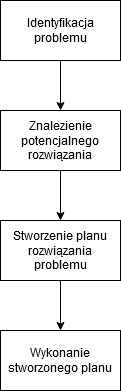
\includegraphics[width=4cm]{images/hyps/diagram-zarzadzania-projektem.png}
	\caption{Uproszczony proces realizacji projektu}
\end{figure}

Powyższy diagram obrazuje proces realizacji projektu w~bardzo skróconym i~uproszczonym formacie, ponieważ każdy etap kryje za sobą wiele kluczowych procesów.

\section {Kim jest menedżer projektu?}
Menedżer projektu, zwany również kierownikiem projektu czy PM (od ang. \emph{project manager}) – jest to specjalista, którego główną odpowiedzialnością jest rozpoczęcie cyklu życia projektu. Zaczyna od przygotowania planu działania, a~następnie wdrożenia go i~zrealizowania, aby ostatecznie móc zamknąć projekt z~sukcesem. Podstawowym zadaniem osoby na stanowisku PM jest zapewnienie wykonania wcześniej zaplanowanych celów, by wydać produkt docelowy, spełniający wszelkie wymagania. Kluczowymi obowiązkami są:

\begin{itemize}
	\item wstępne zaplanowanie projektu, a~następnie jego ustandaryzowanie,
	\item wprowadzenie kluczowych zasad działania,
	\item opracowanie logicznych i~możliwych do zrealizowania celów,
	\item odpowiednie rozporządzenie czasem oraz kosztami. \\
\end{itemize}

W~niektórych przypadkach kierownik projektu zajmuje się również komunikacją z~klientem, aby następnie przedstawić oraz wdrożyć wszelkie jego wymagania. Poza najważniejszymi obowiązkami, dobry kierownik powinien również zadbać o~doskonałą organizację pracy oraz podkreślać, jak ważna jest komunikacja pomiędzy członkami zespołów. Musi rozumieć, że należy skupić się na szukaniu rozwiązań problemów zamiast winnych, a~także pozostać opanowanym, nawet w~najbardziej stresujących sytuacjach.

\section{Cykl życia projektu informatycznego}
Cykl życia projektu to podział na fazy, przez które od początku do końca przechodzi każdy projekt. Zawiera on wszystkie operacje, zadania oraz kroki, których konkretny projekt musi doświadczyć. Zaletami korzystania z~podziału na fazy cyklu życia projektu jest jego efektywna organizacja oraz możliwość ustandaryzowania procesu systematyzacji i~implementacji projektu. Pozwala to na lepszą organizację złożonych projektów informatycznych, poprzez tworzenie i~weryfikowanie modeli dziedziny aplikacyjnej i~samego systemu informatycznego. \cite{IO- Helion}

Cykl życia projektu informatycznego nie zawsze wygląda tak samo. Poszczególne cykle mogą różnić się liczbą faz czy ich nazewnictwem. Najczęściej spotykanym podziałem jest zestawienie na 4-5 fazy. \cite{zarzadzanie5} Są to:

\begin{itemize}
	\item faza planowania,
	\item faza analizy,
	\item faza projektowania,
	\item faza implementacji,
	\item faza testowania. 
\end{itemize}

\subsection {Faza planowania}
Fazą planowania nazywa się pierwszą fazę procesu tworzenia oprogramowania. Jest ona kluczowa, ponieważ pozwala poznać cel oprogramowania oraz sposób jego stworzenia. Już na tym etapie powinny być znane wyniki analizy biznesowej oraz decyzja, czy oprogramowanie może powstać. Dodatkowo, to na tym etapie ustala się wartości dla biznesu, wynikające z~projektu, a~także, czy będzie on opłacalny. Analizuje się również, czy zgromadzone zasoby ludzkie są w~stanie projekt wykonać oraz, czy końcowy produkt będzie możliwy do wdrożenia (co nie jest tak oczywiste już od początku). To na tym etapie zbierane są informacje oraz wymagania od klienta, aby programiści byli w~stanie zdefiniować przeznaczenie systemu. Dochodzi tu do procesu tworzenia opisu systemu w~kategoriach aktorów i~przypadków użycia. Aktorzy to byty zewnętrzne, których zadaniem jest interakcja z~systemem. Natomiast przypadkami użycia nazywa się ogólne sekwencje zdarzeń, odzwierciedlające możliwe sytuacje pomiędzy aktorami a~systemem, bazując na aspekcie jego funkcjonalności.

\begin{figure}[h]
	\centering
	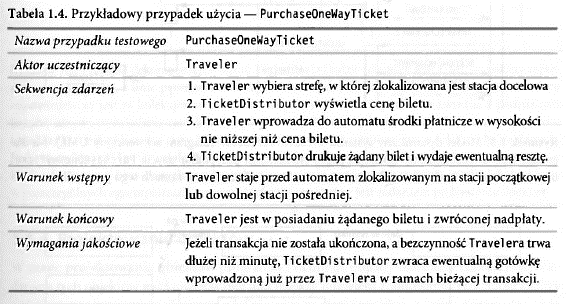
\includegraphics[width=13cm]{images/hyps/use-case.png}
	\caption{Przykładowy przypadek użycia — PurchaseOneWayTicket \\ Źródło:  Inżynieria oprogramowania w~ujęciu obiektowym. UML, wzorce projektowe i~Java, Bernd Bruegge, Allen H. Dutoit}
\end{figure}

\subsection {Faza analizy}
Kolejną fazą jest analiza, w~której przede wszystkim ustala się, kto będzie używał tworzonego systemu, co ona ma robić oraz kiedy i~gdzie będzie używany. Na tym etapie powstaje model, który jest wynikiem zgromadzenia wymagań klienta, jak również wyciągniętych wniosków z~przeprowadzonych przypadków użycia (z~ang. \emph{Use Cases}) Po zakończeniu omawianej fazy, otrzymanym rezultatem jest spójny i~wolny od niejednoznaczności model systemu, wzbogacony o~atrybuty operacji i~skojarzenia. Ewentualne niespójności modelu omawiane są podczas negocjacji z~klientem.

\subsection {Faza projektowania}
W~porównaniu do dwóch poprzednich etapów, w~których główny nacisk kładziony był na ideę stojącą za stworzeniem konkretnego projektu, tak w~teraz, po raz pierwszy pojawia się kreowanie, w~jaki sposób projekt będzie zrealizowany. Tutaj powstają wstępne koncepcje wewnętrznej logiki jego działania. Dochodzi do projektowania interfejsów, m.in. interfejsu użytkownika, a~także omawiana jest cała architektura systemu. Zdarza się, że dochodzi do podziału na dwie mniejsze fazy – projektowania systemu oraz projektowania obiektów.

W~fazie projektowania systemu programiści definiują cele projektu oraz dzielą system na mniejsze podsystemy. Następnie dokonują ewaluacji strategii budowania systemu, co oznacza, że podejmowane są decyzje związane z:

\begin{itemize}
	\item  wyborem platformy sprzętowej oraz systemu operacyjnego środowiska docelowego,
	\item  selekcją technologii użytych i~sposobu przechowywania danych tworzonego oprogramowania,
	\item  globalną kontrolą przepływu sterowania oraz regułą polityki dostępu.
\end{itemize}

Podobnie, jak w~poprzedniej fazie (analizy) – otrzymanym rezultatem jest klarowny opis i~reprezentacja budowanego systemu w~postaci np. diagramu. Główną różnicą jest fakt, że otrzymane modele systemu nie są zrozumiałe dla klienta, jak to było w~fazie analizy. Są one bowiem stworzone za pomocą zaawansowanych i~ulepszonych technik, które mogą być niezrozumiałe przez przeciętnego klienta.

Faza projektowania obiektów ma na celu zasklepienie luk, pomiędzy modelem zbudowanym podczas etapu analizy a~platformą sprzętową i~programową, zdefiniowaną na etapie projektowania systemu. Podczas tej fazy uszczegółowiony oraz sprecyzowany zostaje opis poszczególnych obiektów i~podsystemów w~celu osiągnięcia rozszerzalności, zrozumienia, a~także poprawy wydajności tworzonego systemu. Rezultatem etapu jest szczegółowy model obiektowy, który charakteryzuje się szeroko rozwiniętym spektrum, wyjaśniającym wszystkie elementy.

\subsection {Faza implementacji}
Faza implementacji to w~rzeczywistości wprowadzenie w~życie wszystkich planów, które zostały dotychczas stworzone. W~żargonie programistycznym można powiedzieć, że jest to tłumaczenie modeli na kod źródłowy aplikacji. Oznacza to programowanie każdego obiektu zaprojektowanego w~poprzednich etapach, a~następnie zintegrowanie wszystkich w~jeden działający pojedynczy system. Rezultatem jest zasklepienie przerwy pomiędzy skomplikowanymi i~uszczegółowionymi diagramami, planami oraz modelami, a~skończonym i~skompilowanym kodem źródłowym.

\subsection {Faza testowania}
Ostatnią fazą są testy, wykonywane na stworzonym w~poprzednim etapie, działającym systemie. Polega to na analizie założonych zachowań i~funkcjonalności podczas projektowania, a~rzeczywistym odwzorowaniem w~gotowym oprogramowaniu. To w~tej fazie wykonywana jest zdecydowana większość testów, jednak niektóre były już obecne podczas implementacji. Biorąc pod uwagę liczebność różnych poziomów testów, poniższa grupa jest najpopularniejszą, jeśli chodzi o~projekty informatyczne. Testy dzielone są na:

\begin{itemize}
	\item testy jednostkowe,
	\item testy integracyjne,
	\item testy obciążeniowe,
	\item testy funkcjonalne,
	\item testy akceptacyjne.
\end{itemize}

\subsubsection {Testy jednostkowe}
Zadaniem testów jednostkowych jest sprawdzenie poprawności działania pojedynczego, wyizolowanego bytu. Są to najczęściej pojedyncze funkcje, jednostki lub komponenty. Kluczową cechą tych testów jest brak integracji z~API bądź bazą danych (jest to zadanie testów integracyjnych). Testy jednostkowe muszą działać bardzo szybko (liczone są w~setkach na sekundę), ponieważ używane są przez programistów wielokrotnie w~fazie implementacji. Mają one nie tylko sprawdzać poprawność testowanego komponentu, ale przede wszystkim zapewnić deweloperów, że implementowane przez nich zmiany w~kodzie, nie doprowadzą do usterek funkcjonalnych. \cite{testJ}
\newpage

\begin{figure}[h]
	\centering
	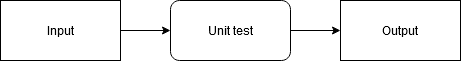
\includegraphics[width=12cm]{images/hyps/unit-test-flow.png}
	\caption{Uproszczony diagram działania testów jednostkowych}
\end{figure}

\subsubsection {Testy integracyjne}
Z~racji podobieństwa, testy integracyjne są często łączone z~testami jednostkowymi. Diametralną różnicą jest fakt, że testy jednostkowe nie sprawdzają integralności między komponentami a~API czy bazą danych, natomiast testy integracyjne – tak. Wykonywane są w~celu wykrycia wad i~defektów w~interfejsach i~komponentach oraz służą do testowania poprawnej interakcji między modułami lub systemami. Są one przeprowadzane w~celu oceny zgodności systemu lub komponentów z~określonymi wymaganiami funkcjonalnymi. Test integracyjny traktuje system jak czarną skrzynkę. Testuje integralność bez zagłębiania się w~szczegóły implementacji, co oznacza, że otrzymywana jest tylko informacja, która konkretna funkcjonalność musi działać oraz co powinno zostać zwrócone jako wynik. Weryfikowane jest, czy otrzymany rezultat zgadza się z~oczekiwanym wynikiem, bazującym na danych wejściowych. Podobnie, jak testy jednostkowe, są tutaj sprawdzane zaimplementowane funkcje oraz poprawność interfejsów, które powinny zapewnić integralność systemu. Mogą one również wskazać błędy w~strukturach danych bądź problemy z~dostępem do API lub bazy danych. \cite{testI}

\subsubsection {Testy obciążeniowe}
Testy obciążeniowe nazywane mogą być również testami wydajnościowymi (ze względu na ich główny cel). Testowana wówczas jest próba obciążenia serwera, bazy danych oraz samego systemu całej aplikacji, bazując na wcześniej przygotowanych scenariuszach użycia oraz wygenerowanych wirtualnych użytkownikach, których zadaniem jest wykonanie wcześniej stworzonych scenariuszy. Przykładowymi scenariuszami użycia są wszelkie działania, które może wykonać klient, np. proces rejestracji czy logowania. Testy obciążeniowe powinny wskazać krytyczne punkty systemu, które w~negatywny sposób wpływają na jego wydajność. Sprawdzają realny ruch na serwerze, który następnie pozwala na zdobycie punktu odniesienia oraz możliwości sprawdzenia, czy projekt spełnia wymogi wydajnościowe. Brak wiedzy z~tego zakresu może doprowadzić do niezaakceptowania projektu do wdrożenia. \cite{testO}

\subsubsection {Testy funkcjonalne}
Testy funkcjonalne opierają się na analizie specyfiki funkcjonalnej tworzonego oprogramowania, systemu lub modułu. Są one najczęściej wykonywane przez osoby, które nie miały styczności z~zaimplementowanym kodem. Testerzy mają za zadanie stworzony system poddać próbie, jednak bez znajomości jego budowy. Głównym zamysłem nie jest przetestowanie konstrukcji czy architektury, lecz założeń funkcjonalnych. Oznacza to, że testerzy powinni wykryć błędy zaimplementowanych funkcjonalności, które zostały zawarte w~dokumentacji. \cite{testF}

\subsubsection {Testy akceptacyjne}
Kolejnym, zupełnie innym rodzajem testów, są testy akceptacyjne. Nie skupiają się na znalezieniu błędów czy pomyłek w~implementacji systemu. Mają potwierdzić wykonanie oprogramowania na odpowiednim poziomie. Służą do uzyskania formalnego potwierdzenia od klienta lub osób zewnętrznych, że wykonany projekt spełnia kryteria jakościowe. Ważnym aspektem jest również weryfikacja, czy w~realizacji nie brakuje założonych w~dokumentacji funkcjonalności oraz czy procesy biznesowe przechodzą w~prawidłowy sposób, czyli budują zaufanie wśród odbiorców. Następnie należy potwierdzić, czy aplikacja jest zgodna z~dokumentacją. Testy akceptacyjne są ostatnim etapem weryfikowania poprawności realizacji systemu informatycznego. To na ich podstawie menedżerowie odpowiedzialni za rozwój projektu podejmują decyzję o~wdrożeniu do użytkowania produkcyjnego. \cite{testA}

\begin{figure}[hb!]
	\centering
	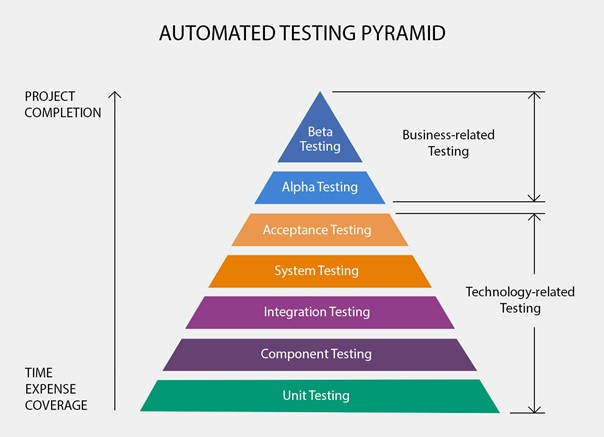
\includegraphics[width=10cm]{images/hyps/test-diagram.jpg}
	\caption{Piramida procesu przeprowadzania testów}
\end{figure}

\section {Metodyki w~projekcie}
Metodyka to zbiór metod, służących do zarządzania projektem. Mówiąc inaczej, są to metody, dzięki którym jest możliwe pozytywne zakończenia projektu w~wyznaczonym czasie. Korzystanie z~metodyki pozwala na uzyskanie maksymalnej wydajności podczas tworzenia oprogramowania. Chociaż jest ich wiele i~wybór zależy stricte od charakterystyki projektu, to w~ramach uproszczenia metodyki można podzielić na grupy. Najogólniejszym i~najpopularniejszym podziałem jest rozdzielenie na klasyczne (nazywane również tradycyjnymi) oraz zwinne. Do pierwszej grupy zaliczymy waterfall, natomiast do drugiej – Agile.

\subsection {Podejście klasyczne a~zwinne}
Aby do realizowanego projektu wybrać metodykę, która pozwoli na skuteczne jego wykonanie, należy znać fundamentalne różnice między wcześniej wymienionymi grupami. Metodyki klasyczne charakteryzują się wysokim stopniem planowania oraz uporządkowania. Projekty są podzielone na konkretne etapy, a~sam harmonogram prac oraz zakres i~cel tworzonego projektu są odgórnie znane. Natomiast metodyki zwinne uznawane są za zupełny kontrast metod tradycyjnych. Nie ma w~tu konkretnego planu, a~praca przypomina swego rodzaju improwizację dostosowaną do zmienności i~losowości okoliczności. Na ich podstawie ukazuje się wcześniej nieznany zakres oraz cel projektu. Grupy te często porównywane są jako uporządkowane i~elastyczne.

Kolejnym faktorem jest rozmiar projektu. W~metodykach klasycznych tworzone są najczęściej duże i~rozbudowane projekty. Wynika to z~faktu, że wielkie przedsięwzięcia wymagają charakterystycznych podejść tradycyjnych, organizacji oraz planowania. Tak, jak zostało to wcześniej wspomniane, sukcesywne realizacje projektu bazują na harmonogramie oraz celach poznanych na początku. W~mniejszych projektach rozmiar, jak i~czas dla przedsięwzięcia, są najczęściej diametralnie mniejsze i~krótsze. Nie wymagają tak ścisłych reguł działania oraz konsekwencji, a~co się z~tym wiąże – metodyki zwinne doskonale do nich pasują.

Kontakt z~klientem w~metodyce klasycznej nie jest konieczny. Występuje on tylko na początku projektu w~fazie zbierania informacji oraz specyfikacji wymagań. A~także na końcu, podczas prezentacji realizacji. W~charakterze zwinnym podejście jest ponownie odmienne – kontakt z~klientem jest ciągły, stąd też wspomniana wcześniej tendencja do zmian w~trakcie projektu. Klienci bowiem zgłaszają swoje opinie oraz zastrzeżenia w~trakcie realizacji, co często doprowadza do przekształcenia zakresu całego projektu.

Zaangażowanie zasobów ludzkich w~obu metodykach ponownie się różni. W~charakterystyce zwinnej nie ma ustalonej hierarchii pracowników, mają oni sporą autonomię, a~współpraca jest dostrzegalna na praktycznie wszystkich płaszczyznach. Metodyka tradycyjna wprowadza hierarchię – w~zespołach występuje osoba (lider), która nie wykonuje tych samych zadań, co pozostali członkowie zespołu. \cite{modele} \cite{agileVwaterfall}

Poniższa tabela w~skondensowany sposób przedstawia kontrast między dwoma metodykami.

\begin{figure}[h]
	\centering
	
\includegraphics[width=13cm]{images/hyps/zwinne-tradycyjne.png}
	\caption{Źródło: Narudo, Zwinne i~tradycyjne zarządzanie projektem}
\end{figure}

\subsection {Metoda waterfall}
Metoda waterfall to przykład modelu kaskadowego, nazywanego również klasycznym. To jeden z~wielu rodzajów procesów tworzenia oprogramowania. Polega na kaskadowym przechodzeniu pomiędzy ukończonymi wcześniej fazami. Zgodnie z~wizją autora tej metodyki, o~sukcesie projektu decydują dokładne zaplanowanie poszczególnych zadań oraz bezwzględne przestrzeganie terminów. Najważniejszym elementem jest tutaj szczegółowy plan oraz dokumentacja dla każdej fazy projektu. Dodatkowo, zakłada on sekwencyjną realizację ustalonych etapów – występują one kolejno po sobie i~tworzą niezależne zadania. W~wyniku braku możliwości przejścia do następnego etapu, przed zakończeniem poprzedniego, występuje wysokie ryzyko pojawienia się błędów, które będą bardzo kosztowne w~naprawie. \cite{waterfall}

\begin{figure}[h]
	\centering
	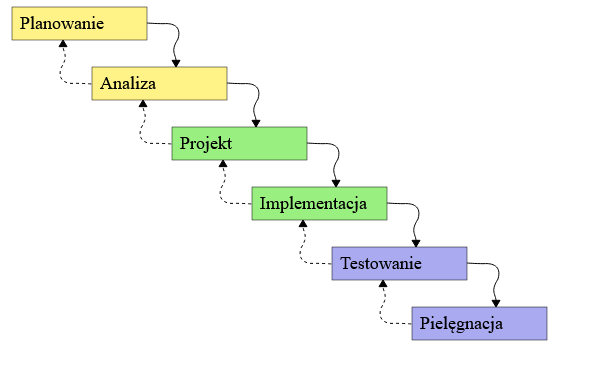
\includegraphics[width=14cm]{images/hyps/waterfall.png}
	\caption{Źródło: Wikipedia, Fazy modelu kaskadowego, Maciej Jaros - Praca własna}
\end{figure}

\subsection{Metody zwinne czyli Agile}
\subsubsection{Manifest Agile}
\begin{center}
\textit{Odkrywamy nowe metody programowania dzięki praktyce w~programowaniu i~wspieraniu w~nim innych. W~wyniku naszej pracy, zaczęliśmy bardziej cenić:\\}
\hfill \break
\textit{\textbf{Ludzi i~interakcje} od procesów i~narzędzi\\}
\textit{\textbf{Działające oprogramowanie} od szczegółowej dokumentacji\\}
\textit{\textbf{Współpracę z~klientem} od negocjacji umów\\}
\textit{\textbf{Reagowanie na zmiany} od realizacji założonego planu.\\}
\textit{Oznacza to, że elementy wypisane po prawej są wartościowe,ale większą wartość mają dla nas te, które wypisano po lewej. \\}
\hfill \break
Żródło: \textit{https://agilemanifesto.org/iso/pl/manifesto.html}
\end{center}

Manifest Agile wprowadzony w~2001 roku zaproponował nowe spojrzenie na możliwości wytwarzania oprogramowania. Przede wszystkim podkreślił wagę pracy zespołowej i~interakcji międzyludzkiej nad dotychczasową koncentracją na procesach i~narzędziach. Zwrócono uwagę na kontakt z~klientem oraz tworzenie roboczego oprogramowania, zamiast wszechstronnej dokumentacji. Największym przeciwieństwem, w~stosunku do dotychczasowych metod, było zaakceptowanie powrotu do fazy implementacyjnej w~celu zareagowania na błędy i~sugestie. \cite{agile} \cite{agile2}

Generalnym założeniem Agile stało się restrykcyjne zarządzanie procesem wytwarzania oprogramowania. Zakładana jest regularna kontrola wymagań oraz rozwiązań, wraz z~procesami adaptacji projektowych. Dużą wagę przywiązuje się do bezpośredniej komunikacji pomiędzy osobami w~zespole oraz codziennego kontaktu między nimi. W~wyniku braku zastosowania jakiekolwiek hierarchii organizacyjnej, na barkach członków zespołu (czyli na osobach realizujących poszczególne zadania) spoczywa większy ciężar dbania o~systematykę i~organizację pracy.

\subsubsection{Czym jest model iteracyjny w~Agile?}
Podejście zwinne jest grupą metod, które bazują na tworzeniu oprogramowania. Oparte jest na stylu iteracyjno-przerostowym. Głównym jego założeniem jest tworzenie i~wdrażanie systemu etapami. Pojedyncza iteracja kończy zrealizowany cykl życia projektu etapem testów. Wówczas zrealizowana już część zostanie przekazana odpowiedniej grupie, odpowiedzialnej za przeprowadzenie sprawdzenia poprawności działania. Testowana jest również praktyczność zastosowania faktycznych założeń biznesowych. Zdobywanie regularnej informacji zwrotnej, pozwala na cykliczne korekty błędów, wprowadzanie zmian i~ulepszeń funkcjonalności oraz precyzyjne reakcje na potrzeby klienta. Stąd wspomniane wcześniej tendencje do ewolucji funkcjonalności w~projekcie. Pojedynczy cykl rozpoczyna się od fazy szczegółowego planowania zadań rozłożonych w~konkretnym cyklu. Najczęściej przygotowywany jest przez szefów zespołów programistycznych lub kierowników projektowych. Następnym krokiem jest implementacja wcześniej przygotowanych założeń i~funkcjonalności, po której nadchodzi czas na testy i~wdrożenie. To tutaj docelowa grupa bada jakość przygotowanej cząstki projektowej i~decyduje o~możliwości wdrożenia oraz przejścia do kolejnej iteracji.

\begin{figure}[h]
	\centering
	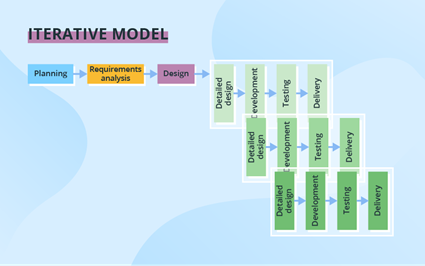
\includegraphics[width=13cm]{images/hyps/iterative-model.png}
	\caption{Źródło: ScienceSoft, Model iteracyjny \cite{wykresy}}
\end{figure}

Powyższy model obrazuje podejście iteracyjne, które jest charakterystyczne w~metodyce Agile.

\section{Wykorzystanie Agile w~tworzeniu gry}
\subsection{Agile Game Development}
Agile Game Development to angielska nazwa na wykorzystanie podejścia zwinnego w~tworzeniu gry komputerowej. Samo podejście nie różni się niczym szczególnym od standardowego, kluczowe jest natomiast pokazanie, jak wiele możliwości wprowadza Agile do życia projektu gry. Główną z~nich jest wcześniej rozwinięty model iteracyjny. Dzięki niemu cząstki gry, charakteryzujące się nowymi funkcjonalnościami, znacznie częściej trafiają na testy do grupy docelowej. Takie podejście zwykle pozwala naprawić wiele błędów, których nie udało się wykryć w~fazie implementacji oraz poprawić działanie licznych funkcjonalności. Podczas realizacji zadań i~rozwijania gry programista może wpaść w~pułapkę subiektywnej opinii, dotyczącej zaimplementowanych rozwiązań. Jak to zwykle się zdarza, bywają one błędne i~możliwość ich weryfikacji na tak początkowym etapie – wprowadza ogromną wartość w~projekcie. Pomimo przypisania takich elementów, jak model iteracyjny czy częsty kontakt z~klientem do podejścia zwinnego, to w~rzeczywistości są to nadrzędnymi składowymi metod, z~których składa się metodyka Agile (przypominając, metodyka to zbiór wcześniej założonych metod). W~projekcie „The Lore” została wykorzystana fuzja trzech najpopularniejszych metod. Jest to najbardziej powszechna i~najczęściej wykorzystywana strategia w~projektach komercyjnych. \cite{Agile game}\cite{agilePract} Do tej grupy należą:

\begin{itemize}
	\item SCRUM,
	\item Kanban,
	\item XP —  Programowanie Ekstremalne.
\end{itemize}

\subsubsection{SCRUM}

Scrum to zdecydowanie kluczowa i~prawdopodobnie najważniejsza część Agile. To ona jest odpowiedzialna za zarządzanie procesem iteracyjnym w~projekcie. Jednak w~tym przypadku pojedyncze iteracje nazywane są sprintami, czyli wcześniej zdefiniowanymi partiami pracy, posiadającymi przypisane do nich zadania oraz wydzielone terminy. Sprinty trwają najczęściej od dwóch do czterech tygodni, w~zależności od zarządzeń czy planów biznesowych. Sprinty w~początkowej fazie prac w~przypadku „The Lore”, czyli na etapie około trzech miesięcy, trwały dwa tygodnie, a~następnie zostały zredukowane do tygodnia. Wynikało to ze wzrostu jakości otrzymywanego produktu, ponieważ był on częściej oddawany w~ręce testerów, a~także sam proces programistyczny mógł być lepiej rozplanowany. Pozwalało to na przypisanie sprintów do wykonania konkretnych funkcjonalności, zamiast tworzenia przeładowanego sprintu z~różnymi funkcjonalnościami. Tym samym wzrosła wydajność pracy, ponieważ grupa docelowa oczekiwała już gotowego uaktualnienia produktu. Kolejnym doskonałym elementem Scrum jest wprowadzenie ról dla poszczególnych członków zespołu. W~podejściu zwinnym brakuje hierarchizacji w~zespole, co może ostatecznie doprowadzić do katastrofy organizacyjnej. \cite{agileHunt} Dlatego też Scrum wprowadza trzy funkcje:

\begin{itemize}
	\item Scrum Master,
	\item właściciel produktu,
	\item zespół deweloperski.
\end{itemize}

Scrum Master to osoba odpowiedzialna przede wszystkim za przestrzeganie zasad Scrumowych. W~omawianym projekcie diametralnie wpłynął na wydajność i~produktywność zespołu, ponieważ wielokrotnie podczas sprintów, pilnował postępów prac oraz jakości ich wykonania. Zajmował się również komunikacją ze źródłami zewnętrznymi, aby pozostałe osoby z~zespołu nie musiały tracić na to czasu i~odrywać się od pracy. Do jego obowiązków należało również planowanie szczególnych spotkań, tak zwanych retrospektyw oraz przeglądów sprintów.

Retrospektywa to spotkania, odbywające się cyklicznie co 2-3 tygodnie, w~celu ustalenia organizacji pracy czy dyskusji o~odczuciach każdego członka zespołu. Czasami bywały to rozmowy stricte związane z~kodem, jednak bywały też takie, które dotyczyły jakości pracy, bądź kontaktów interpersonalnych. W~dużym uproszczeniu, retrospektywa to czas dla zespołu, w~którym może przedyskutować realizację, wady i~zalety oraz to, jakie można podjąć kolejne kroki rozwiązujące ewentualne problemy.

Przegląd sprintu również jest cyklicznym spotkaniem, jednak odbywał się częściej – po każdym zakończonym sprincie. Jego głównym zadaniem jest dyskusja członków zespołu o~stworzonych przez nich funkcjonalnościach. Omawiany jest sposób podejścia dewelopera do danych zadań oraz ich realizacja. Dzięki temu w~sytuacji, gdy inna osoba z~zespołu otrzymała zadanie rozwoju tej funkcjonalności w~kolejnym sprincie, miała już przygotowaną bazę wiedzy, wystarczającą do realizacji. Pozwala to znacznie zaoszczędzić czas, potrzebny do zrozumienia działania kodu, napisanego przez innego członka zespołu. Podczas przeglądu sprintów tworzony jest również kolejny sprint, w~którego skład wchodzą zadania, bazujące na tworzeniu funkcjonalności zgodnie z~harmonogramem. Po wypełnieniu nowego sprintu konkretnymi zadaniami, dochodzi do rozmowy o~przydziale ich do konkretnej osoby. Głównymi czynnikami doboru zadań do członków zespołu, było ich doświadczenie w~pracy z~zadaniami łączonymi bądź zależnymi, które były wykonane we wcześniejszych sprintach.

Właścicielem produktu jest najczęściej osoba niebędąca w~zespole, a~tylko zlecająca wykonanie projektu. Jednak w~przypadku gry „The Lore” ten tytuł spoczywał na barkach członka zespołu. Jego zadaniem było zadbanie o~klarowną wizję projektu i~pilnowanie, czy tworzony jest zgodnie z~ustaleniami. Odpowiadał również za rozwój, jak i~maksymalizację wartości produktu. Robił to, decydując o~kolejności wykonywania prac i~wprowadzanych funkcjonalnościach. Zarządzał również ich priorytetami i~treściami tworzonych zadań. Wykonywał to wraz z~Scrum Masterem, jednak to decyzja właściciela była najważniejsza. Projekt był tworzony i~rozpisany zgodnie z~jego wizją produktu finalnego.

Ostatnią grupą odpowiedzialną za realizację projektu jest zespół deweloperski. Charakterystyką tej roli jest dostarczenie przygotowanej, gotowej do wydania, aktualizacji projektu. Ten zespół realizuje backlog sprintu przygotowanego wcześniej podczas przeglądu sprintów.

\begin{figure}[h]
	\centering
	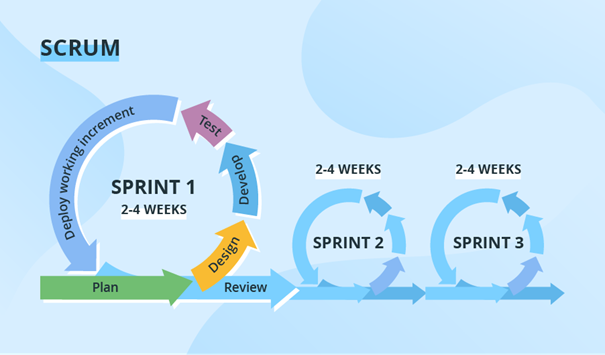
\includegraphics[width=13cm]{images/hyps/scrum.png}
	\caption{Źródło: ScienceSoft, SCRUM \cite{wykresy}} 
\end{figure}

Na powyższym zdjęciu prezentowany jest cykl realizacji sprintów oraz poglądowa wizaulizacja modelu pracy w~Scrum'ie.

\subsubsection{Kanban}
Kanban to kolejna z~metod w~metodyce Agile. Jej głównym założeniem jest wizualizacja procesu realizacji zadań. Podczas projektowania „The Lore”, przy użyciu tzw. tablicy kanbanowej, obrazowano, w~którym etapie znajduje się poszczególne zadanie. Tablica została podzielona na najprostszy układ tj. podział na czynności „do zrobienia”, „w trakcie realizacji” i~„zrobione”. Jej celem było doprowadzanie do sytuacji, w~której organizacja pracy poszczególnych osób z~zespołu, jest widoczna dla wszystkich. Dzięki temu proces realizacji zadań od siebie zależnych przechodził w~bezproblemowo i~jawnie. Jednocześnie dawało to wizualne potwierdzenie, na jakim etapie pracy jest każdy członek zespołu. Przy niezadowalającym tempie realizacji zadań, w~pracę zespołu interweniował Scrum Master lub właściciel produktu. \cite{kanban}
\newpage
\begin{figure}[h]
	\centering
	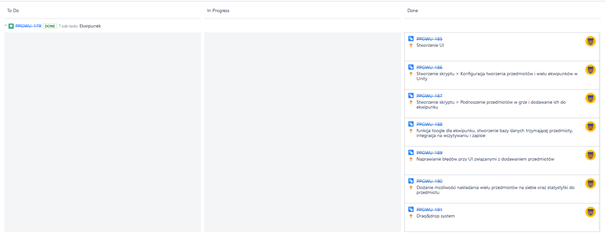
\includegraphics[width=13cm]{images/hyps/jira.png}
	\caption{Tablica kanbanowa w~programie Jira. Przykład z~projektu ,,The Lore''}
\end{figure}

„Jira to platforma do organizowania pracy i~uruchamiania oraz monitoringu procesów w~organizacjach.”  \cite{jira} Pozwala na utworzenie tablicy kanbanowej i~zarzadzania nią w~projektach. 

\subsubsection{Programowanie ekstremalne}
Programowanie ekstremalne to już ostatnia metoda użyta w~realizacji projektu „The Lore”. Skupia się na adaptacji do częstych zmian, wynikających z~cyklicznych aktualizacji projektu. Głównym założeniem, które zostało wykorzystane, jest „pair programming”, czyli programowanie w~parze (lub nawet większej grupie ludzi). Dzięki wspólnemu planowaniu, dyskutowaniu o~potencjalnym rozwiązaniu, a~następnie zaimplementowaniu – zmniejsza się czas potrzebny na wykonanie zadania, które normalnie byłoby tworzone przez pojedynczego dewelopera. Jest to szczególnie użyteczne, gdy zbliża się termin zakończenia sprintu, a~zadanie jest nadal we wczesnej fazie, lub gdy deweloper natrafił na „ślepy zaułek” i~potrzebuje świeżego spojrzenia na zadanie.

\subsection{Cykl życia projektu ,,The Lore''}

\subsubsection{Faza zbierania informacji i~analizy}

Podczas pierwszych faz realizacji projektu „The Lore” tworzona była szeroka dokumentacja, której zadaniem było zebranie jak najwięcej informacji, potrzebnych do obrania odpowiedniego kierunku prac. Dzięki temu właściciel produktu wraz ze Scrum Masterem mieli potencjalną wizję na tworzony harmonogram i~przygotowanie backlogu z~zadaniami na najbliższe sprinty. Dokumentacja, wraz z~później przygotowanymi na jej podstawie \emph{user stories}, była w~tej fazie kluczowa. W~jej skład wchodziła wizja projektu, VPC oraz BMC.

\textbf{Dokument wizji projektu} – jego nadrzędnym założeniem jest przedstawienie przeznaczenia tworzonego oprogramowania oraz głównych cech i~przyjętych założeń. Dokument dzieli się na sekcje: wprowadzenia, celu projektu, badania rynku, użytkowników docelowych, szczegółowego opisu produktu wraz z~zakresem i~ograniczeniami.

\textbf{Value Proposition Canvas} (VPC) to angielska nazwa na przedstawienie unikalnej propozycji wartości modelu biznesowego. Celem jest łatwiejsza analiza i~zaprojektowanie produktu wraz z~jak najtrafniejszym skonfigurowaniem rozwiązań pod potrzeby klientów. \cite{VPC}
\begin{figure}[h]
	\centering
	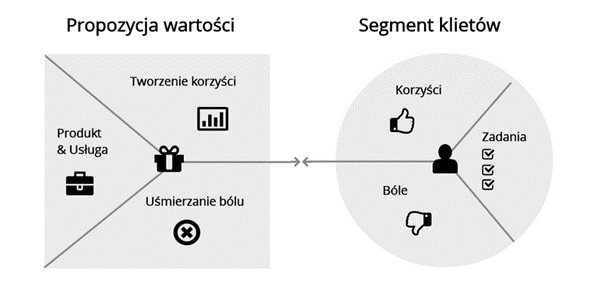
\includegraphics[width=10cm]{images/hyps/VPC.png}
	\caption{Źródło: Product Vision, Value Proposition Canvas}
\end{figure}

\begin{figure}[hb!]
	\centering
	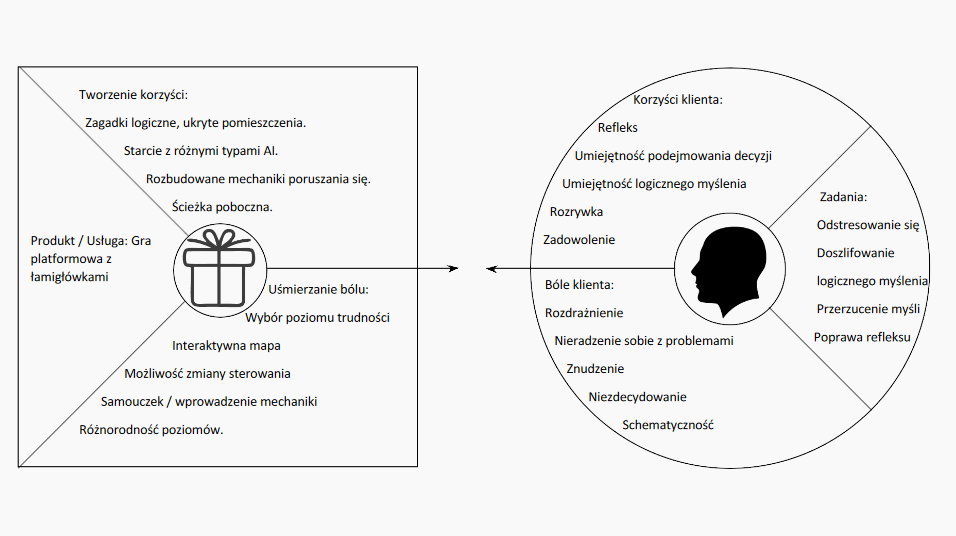
\includegraphics[width=11cm]{images/hyps/VPC-The Lore.png}
	\caption{Value Proposition Canvas dla projektu ,,The Lore''. Przykład z~,,The Lore''}
\end{figure}
Powyżej przedstawiony jest przykład unikalnej propozycji wartości modelu biznesowego oraz już oficjalny model z~projektu gry "The Lore".

\textbf{Business Model Canvas} (BMC) to, podobnie jak VPC, angielska nazwa na szablon modelu biznesowego. Jego zadaniem jest przedstawienie w~wizualny sposób, jak planowany projekt ma przynieść zyski. Składa się z~9 podstawowych obszarów, które obrazują grupę docelowych użytkowników oraz sposób, w~jaki zostanie im dostarczony produkt. Jednocześnie pokazuje wszelkie korelacje z~wydatkami, jak i~potencjalnymi zarobkami planowanego projektu. \cite{BMC}

\begin{figure}[h]
	\centering
	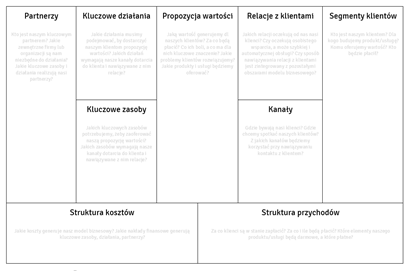
\includegraphics[width=13cm]{images/hyps/BMC.png}
	\caption{Źródło: Product Vision, Business Model Canvas}
\end{figure}

Powyżej przedstawiony jest przykładowy szablon modelu biznesowego. Natomiast poniżej już oficjalny model z~projektu gry "The Lore".
\newpage
\begin{figure}[h]
	\centering
	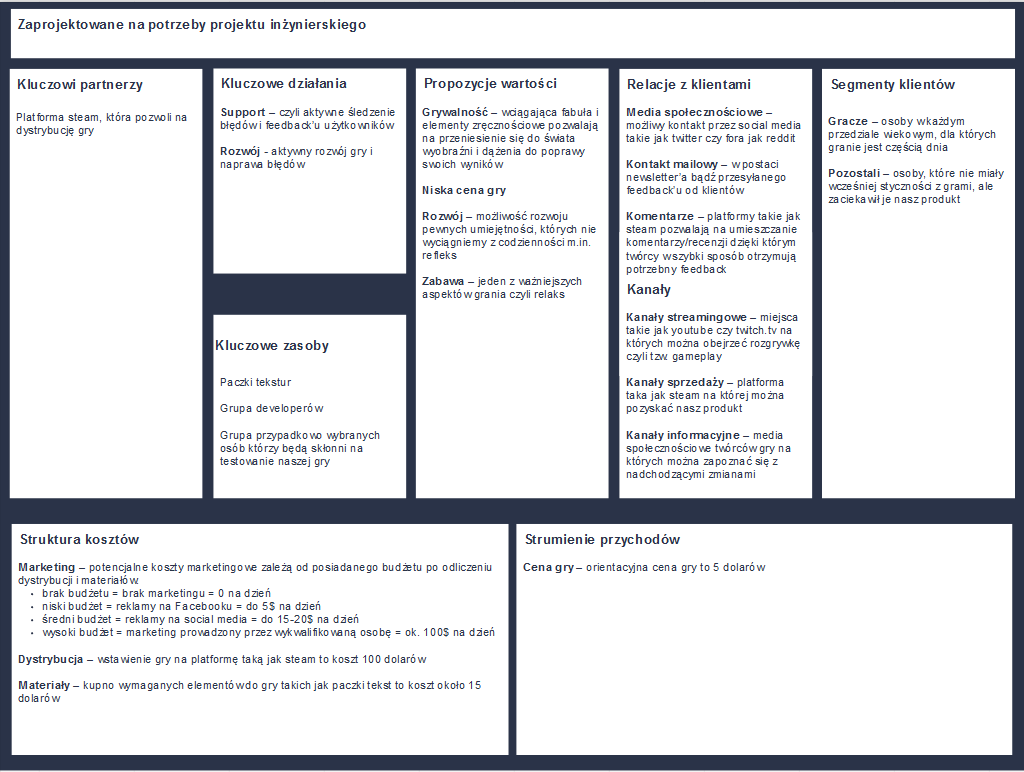
\includegraphics[width=13cm]{images/hyps/BMC - The Lore.png}
	\caption{Business Model Canvas dla projektu ,,The Lore''. Przykład z~,,The Lore''}
\end{figure}

Utworzone \emph{user stories} zostały wykorzystane do realizacji pierwszych pierwszych zadań w~backlogu projektu.

\begin{figure}[hb!]
	\centering
	
\includegraphics[width=13cm]{images/hyps/backlog.png}
	\caption{Backlog z~zadaniami w~programie Jira. Przykład z~,,The Lore''}
\end{figure}

\subsubsection{Faza projektowania}

Po zakończeniu dwóch poprzednich faz, w~których rozwijany był zamysł stworzenia gry komputerowej „The Lore”, przyszedł czas na skupienie się na tym, w~jaki sposób zostanie ona zaprojektowana.

Pierwszą rozterką było wybranie odpowiedniego środowiska. Pośród wielu możliwości na rynku, wybór padł na Unity. Miał on opinię najbardziej przyjaznego dla początkujących twórców gier komputerowych, a~także najlepiej rozwiniętą dokumentację techniczną i~największą bazę użytkowników udzielających się na specjalistycznych forach. Unity posiada również autorski sklep z~materiałami, które są nieocenione przy tworzeniu gry w~ograniczonym czasie.

Po wybraniu środowiska następną decyzją jest wybór odpowiedniego języka programowania. Jednak nie było to zadanie trudne, ponieważ z~grupy Boo, UnityScript oraz C\# – tylko ten ostatni był nadal wspierany przez Unity oraz cieszył się największą popularnością wśród twórców. Był to również najlepiej znany język w~grupie deweloperskiej.

Kolejny etap to wybór docelowej technologii oraz systemów, na które ma trafić wdrożony projekt. Estymowany był tutaj dostępny czas oraz wymagania, jakie kryją się za tworzeniem gry jednocześnie na urządzenia mobilne, stacjonarne, jak i~konsole. Niezależnie od możliwości, jakie posiada Unity, dla budowania projektu na różne platformy, sama implementacja funkcjonalności stwarzała komplikacje. Wynikały one z~unikalnych cech każdej platformy. Stąd została podjęta decyzja o~wykonaniu gry na pojedynczą platformę – stacjonarną, ale z~kompatybilnością na trzy najpopularniejsze systemy operacyjne: Windows, Linux, MacOS.

Następnym etapem projektowania technicznego było dobranie odpowiedniej platformy wdrożeniowej. Na rynku jest ich wiele, a~różnice są często marginalne i~zależą od różnych twórców czy cen za wdrożenie autorskiego projektu. Dylematem było wykorzystanie drogiego, lecz jednocześnie najpopularniejszego miejsca na dystrybucję gry, bądź wykorzystanie mało znanych platform, które udostępniają możliwość wdrożenia produktu za darmo. W~związku z~dosyć ograniczonym budżetem projektowym, wybór musiał paść na platformę mniej znaną.

Niezbędną decyzją był wybór platformy do przechowywania plików. Przy projektach tworzonych w~pojedynkę, takie miejsce służy do bezpiecznego przechowywania progresu prac. Jednak przy pracy w~zespole, celem jest również współdzielenie danych i~szybki dostęp do plików projektu. Najpopularniejszym na rynku środowiskiem jest Github. Wymagał on jednak specjalnej konfiguracji, ponieważ pliki przekazywane przez Unity są odmienne od standardowych. Edytor Unity tworzy setki tymczasowych plików, które nie zawsze powinny trafić na Githuba. Odpowiednia konfiguracja pliku \emph{gitignore}, którego celem jest nieprzesyłanie wpisanych tam rozszerzeń, typów plików czy folderów – była kluczowa. Kolejnym problemem, który trzeba było rozwiązać, były błędne referencje do specjalistycznych obiektów w~Unity. Tego typu informacje wysyłane były na Githuba w~specjalnych plikach z~rozszerzeniem .meta, które rozwiązały wszelkie problemy ze znikającymi obiektami, stworzonymi przez programistów. Ostatnim i~największym problemem była konfliktowość wynikająca z~edycji tych samych plików binarnych przez wielu programistów. Rozwiązanie ich podczas prób \emph{mergu branchy} było niemożliwe. Stąd kluczowa była komunikacja wewnątrz zespołowa, wraz z~odpowiednią organizacją pracy i~umiejętnym podziałem zadań. W~fazie projektowania zostały stworzone również pierwsze szkice interfejsów graficznych. Wiele z~nich zostało później zmodyfikowanych lub zupełnie zmienionych.

Poniżej przedstawione są zdjęcia prototypów interfejsów graficznych głównego menu oraz menu sterowania.

\begin{figure}[h]
	\centering
	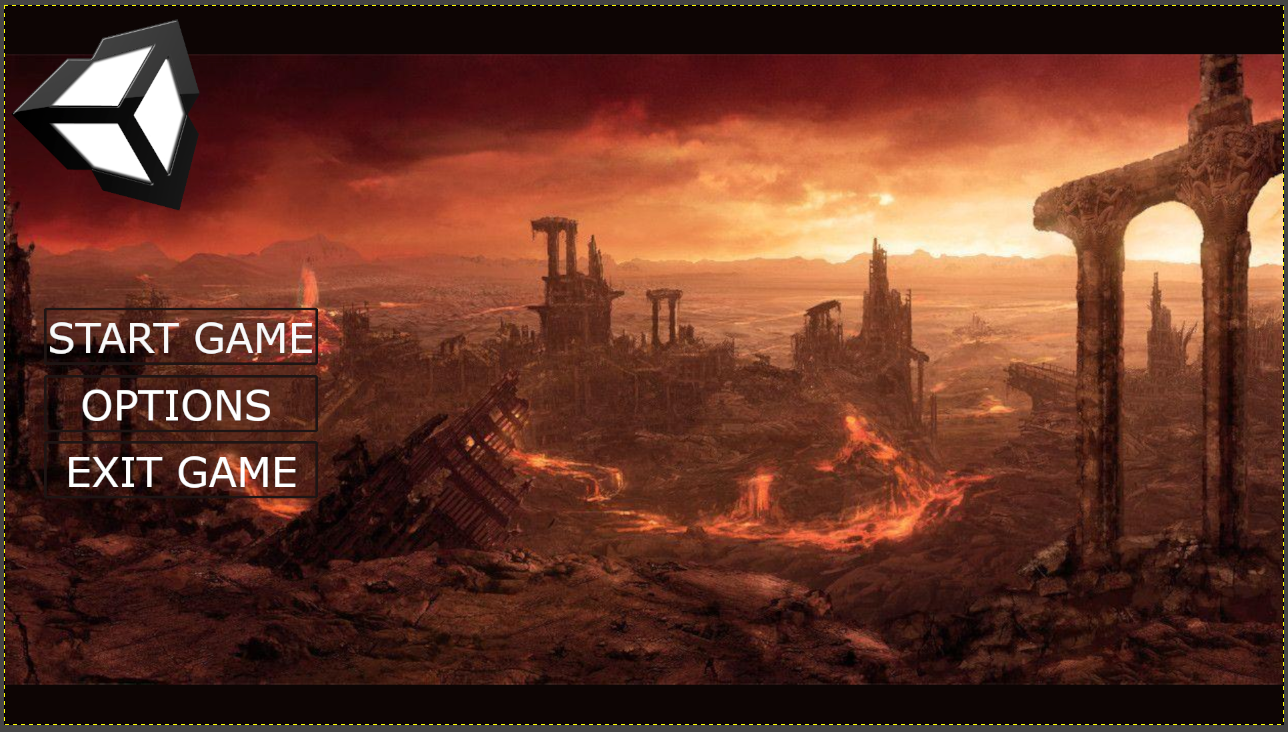
\includegraphics[width=13cm]{images/hyps/proto.png}
	\caption{Prototyp interfejsu menu głównego. Przykład z~,,The Lore''}
\end{figure}
\newpage
\begin{figure}[ht!]
	\centering
	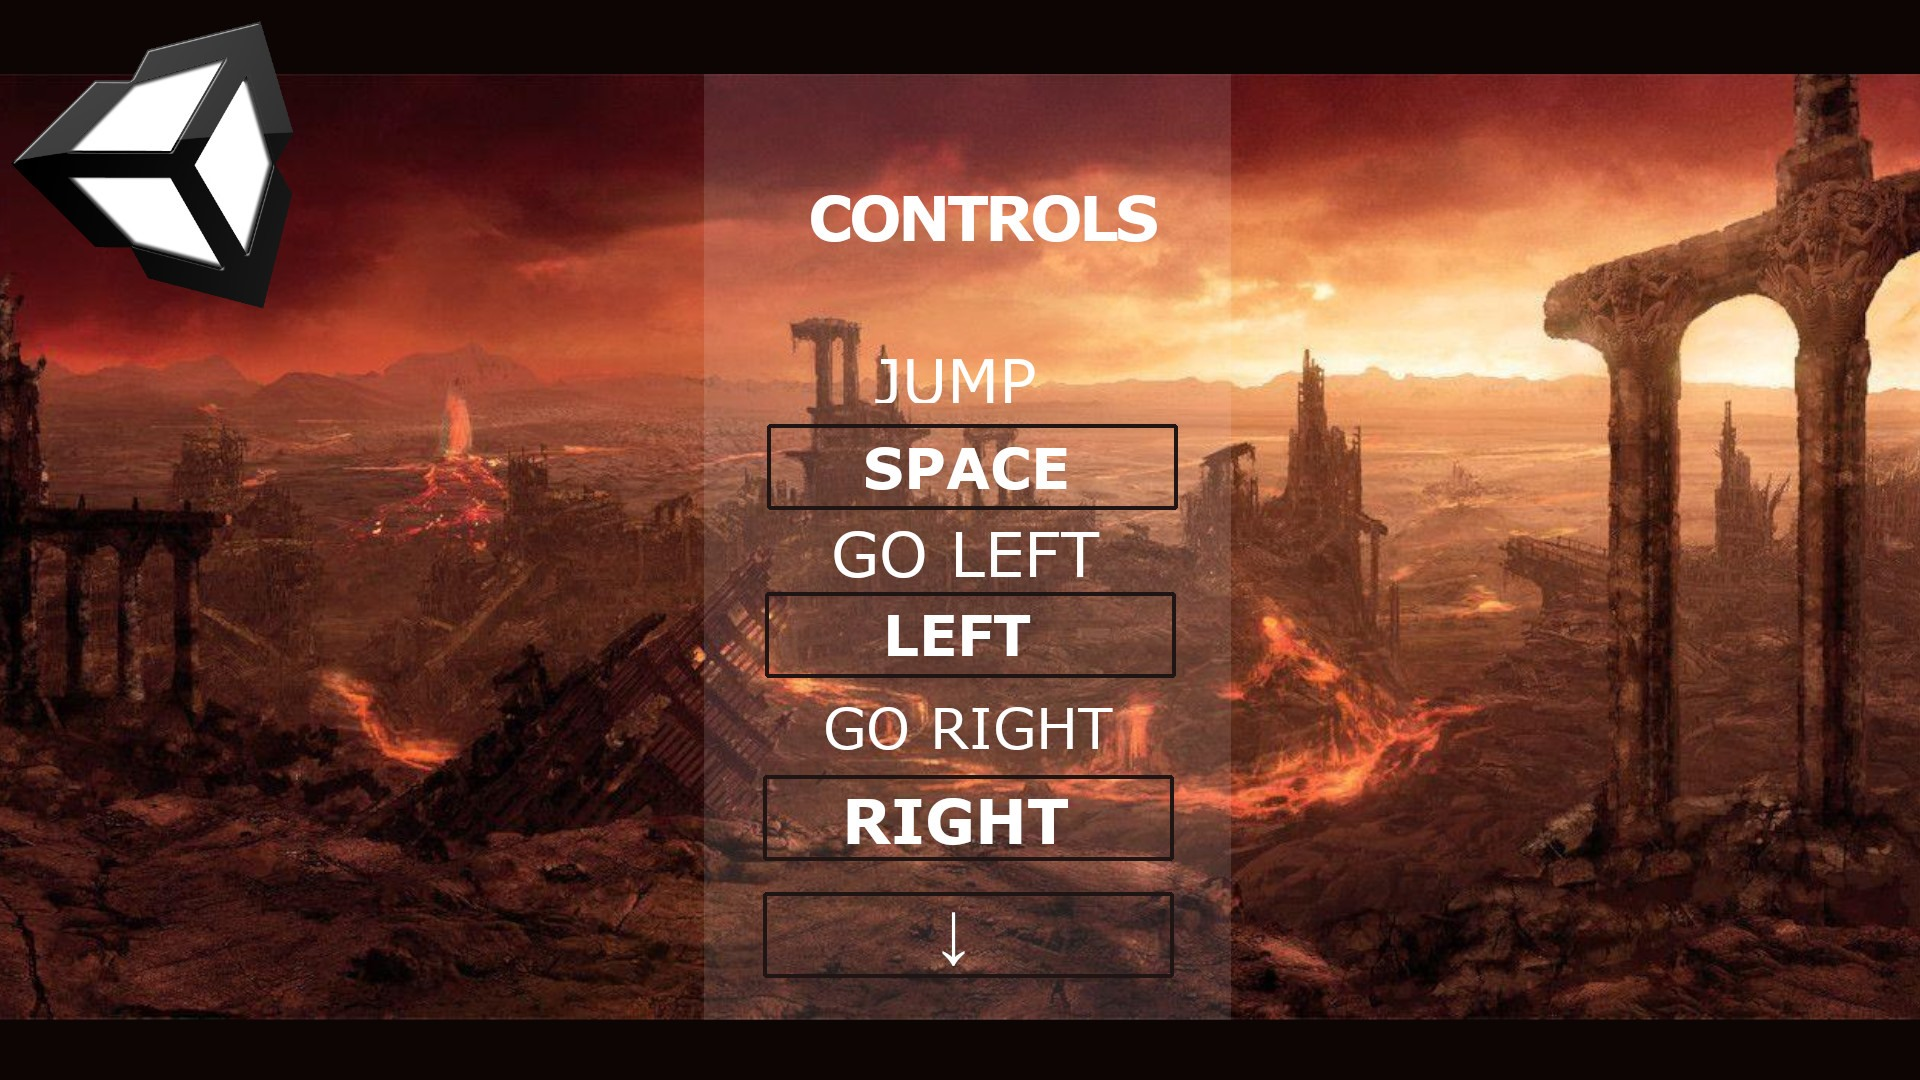
\includegraphics[width=13cm]{images/hyps/proto2.jpg}
	\caption{Prototyp interfejsu menu sterowania. Przykład z~,,The Lore''}
\end{figure}

Poniżej przedstawione są zdjęcia z~już wdrożonych interfejsów graficznych głównego menu oraz menu sterowania.

\begin{figure}[hb!]
	\centering
	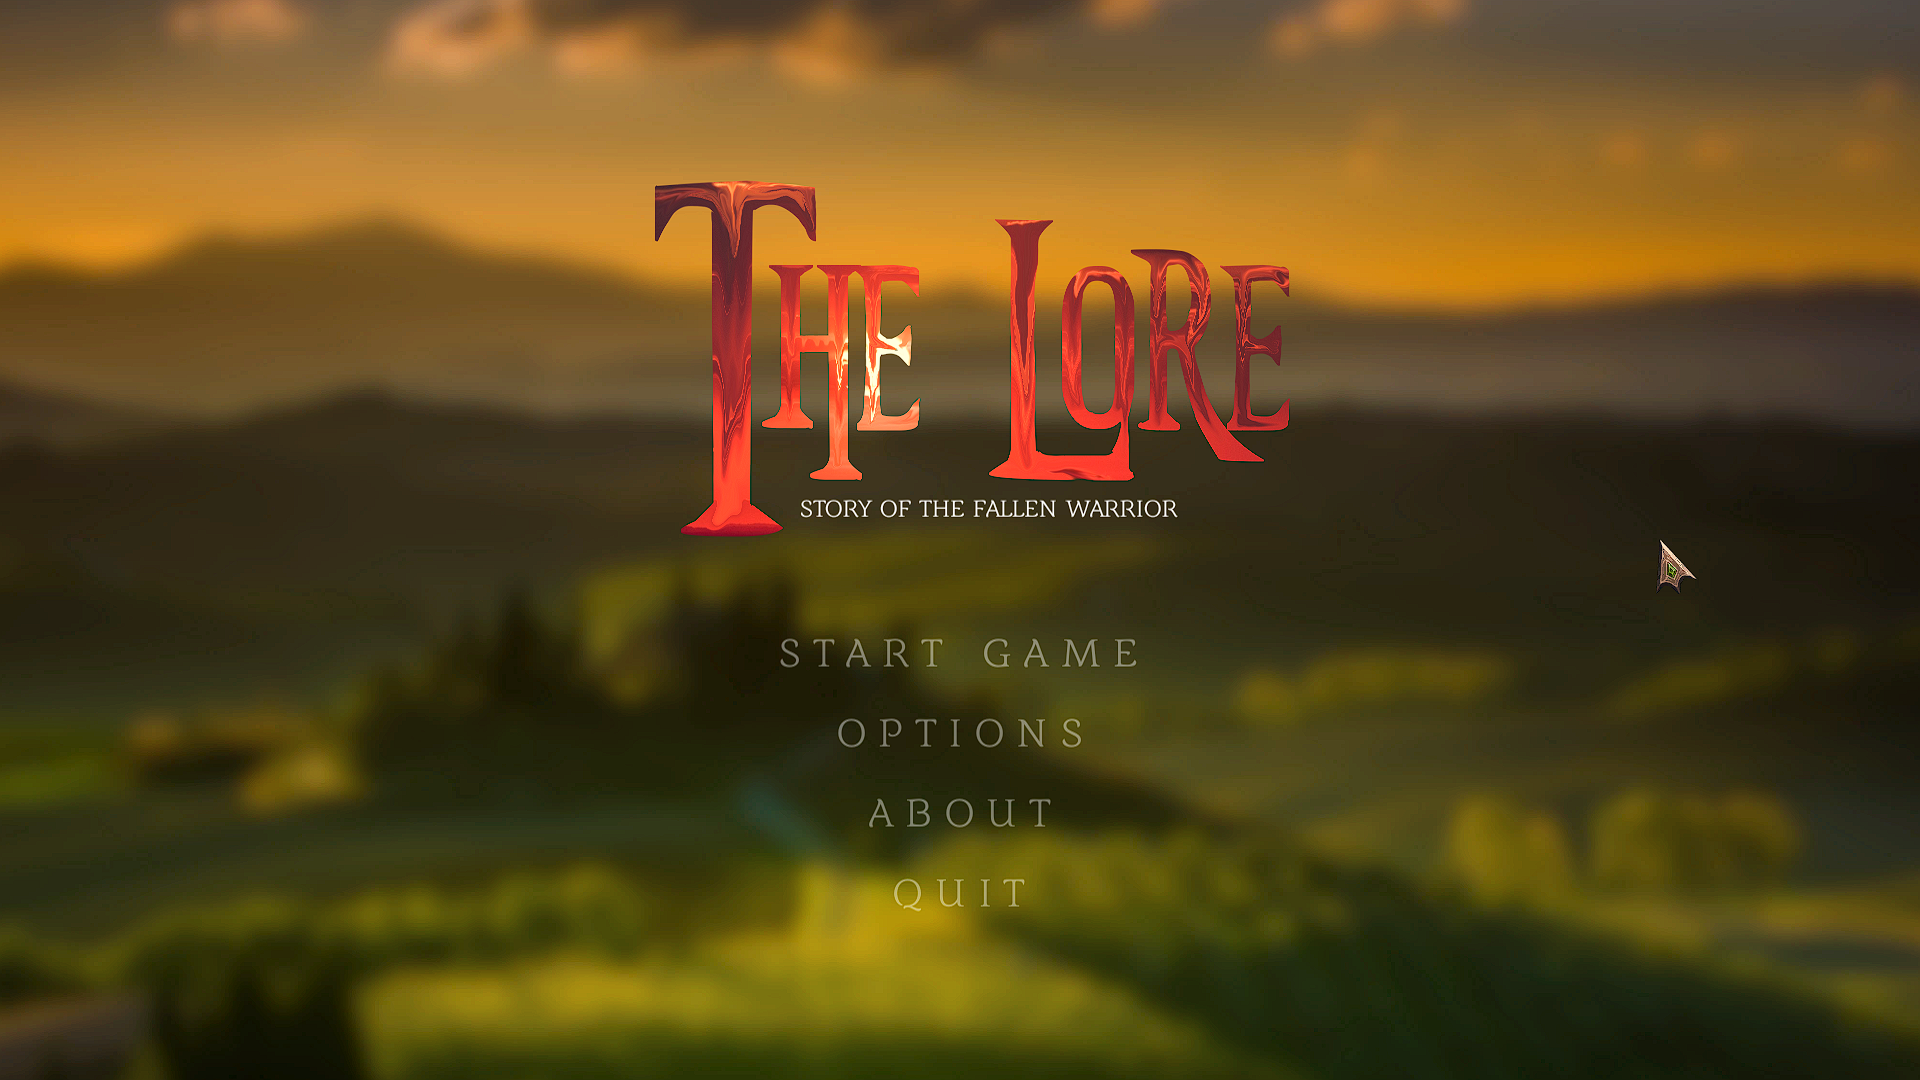
\includegraphics[width=13cm]{images/hyps/of1.png}
	\caption{Wdrożony interfejs menu głównego. Przykład z~,,The Lore''}
\end{figure}
\newpage
\begin{figure}[ht!]
	\centering
	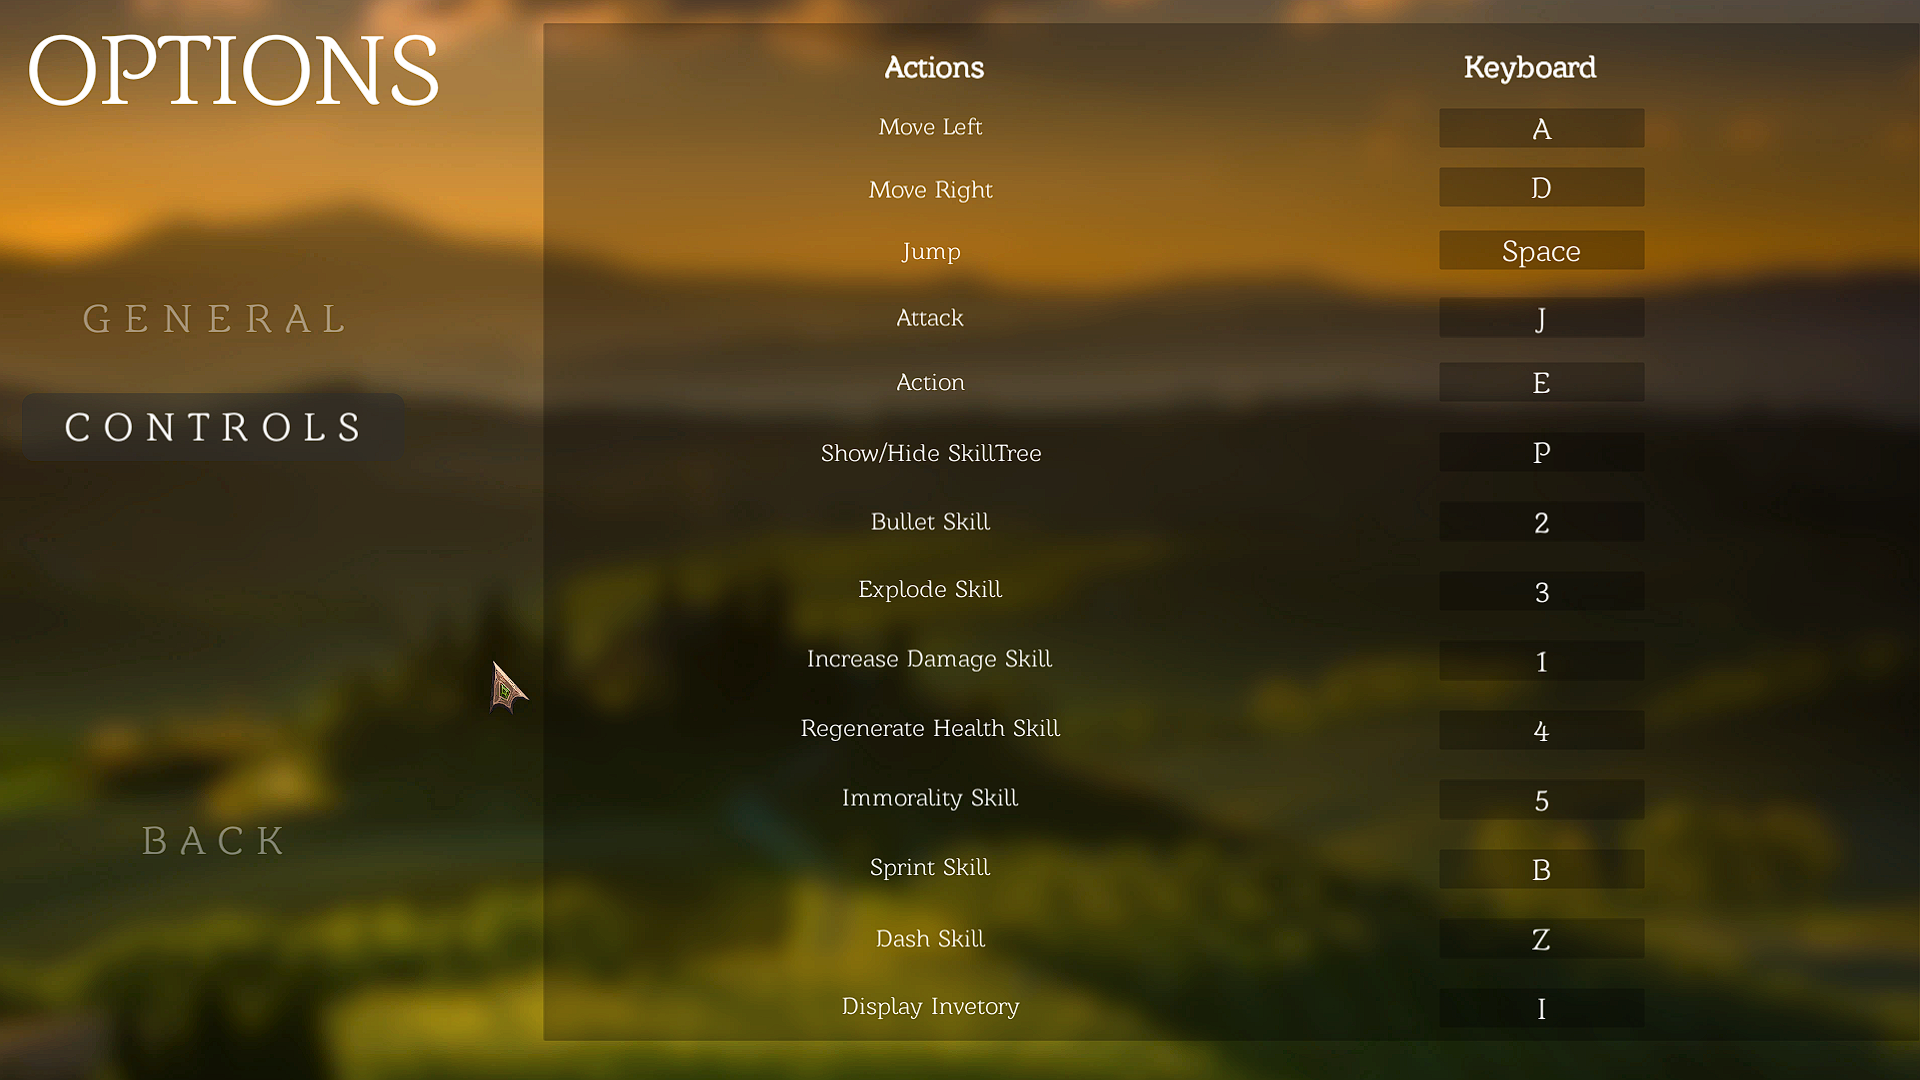
\includegraphics[width=13cm]{images/hyps/of2.png}
	\caption{Wdrożony interfejs menu sterowania. Przykład z~,,The Lore''}
\end{figure}

\subsubsection{Faza implementacji i~testów}

Faza implementacji oraz testami powtarzana była wielokrotnie w~wyniku metodyki Agile. Poprzez model iteracyjny, każdy sprint wykorzystywany był do zaimplementowania wcześniej zaprojektowanych funkcjonalności oraz przedstawienia ich grupie testerów. Dzięki temu w~projekcie gry „The Lore” zespół deweloperski był w~stanie na bieżąco wprowadzać wszelkie poprawki wraz z~sugestiami otrzymywanymi podczas testów. Przykładową funkcjonalnością jest element poziomu samouczka – poruszające się platformy. Zgodnie z~powtarzającą się opinią o~trudności w~przechodzeniu tego elementu, zostały wprowadzone poprawki oraz dodatkowe ułatwienia. Przykładowym rozwiązaniem było dodanie specjalistycznej fizyki, która miała na celu przyciąganie gracza w~kierunku nadchodzącej platformy. Innym, bardziej wizualnym ułatwieniem, było dodanie tras, po których poruszają się platformy. Ostatnim ułatwieniem było zmniejszenie prędkości poruszania się platform oraz powiększenie ich powierzchni.

Poniżej przedstawiono zdjęcia z~pierwszej i~ostatniej iteracji tworzonej funkcjonalności, która odzwierciedla zmiany po otrzymanych uwagach z~fazy testów.
\newpage
\begin{figure}[h]
	\centering
	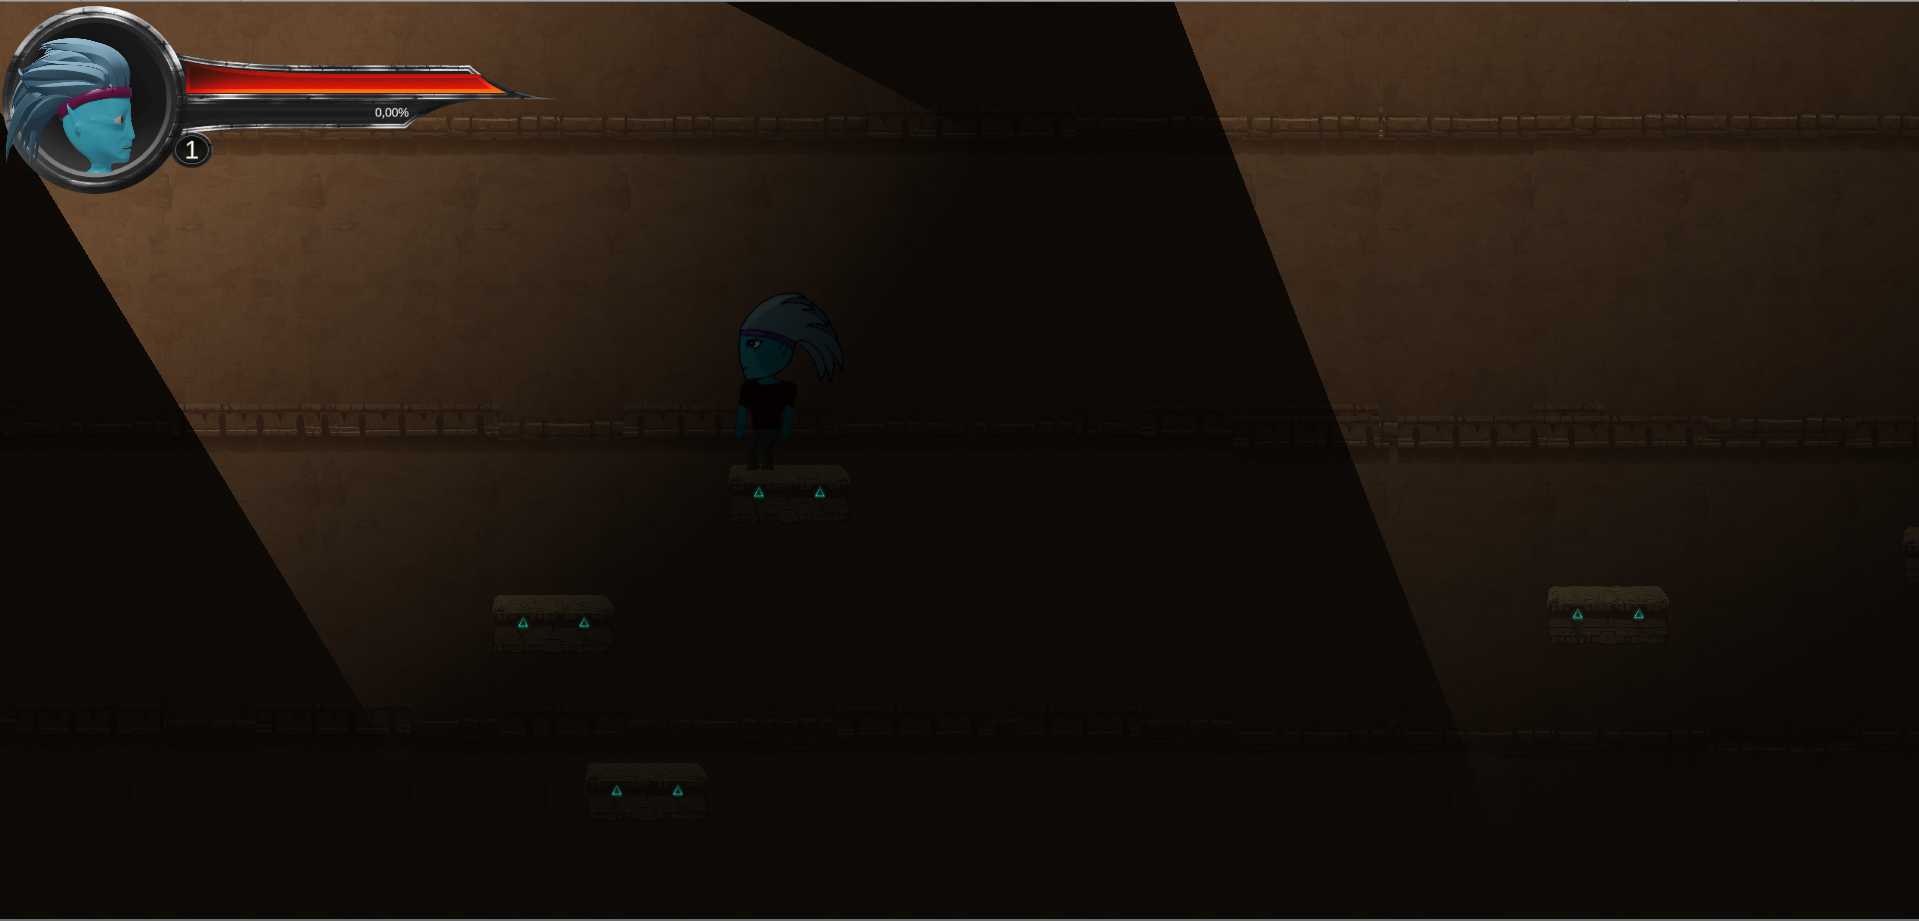
\includegraphics[width=13cm]{images/hyps/platfBef.png}
	\caption{Pierwsza iteracja ruchomych platform. Przykład z~,,The Lore''}
\end{figure}

\begin{figure}[h!]
	\centering
	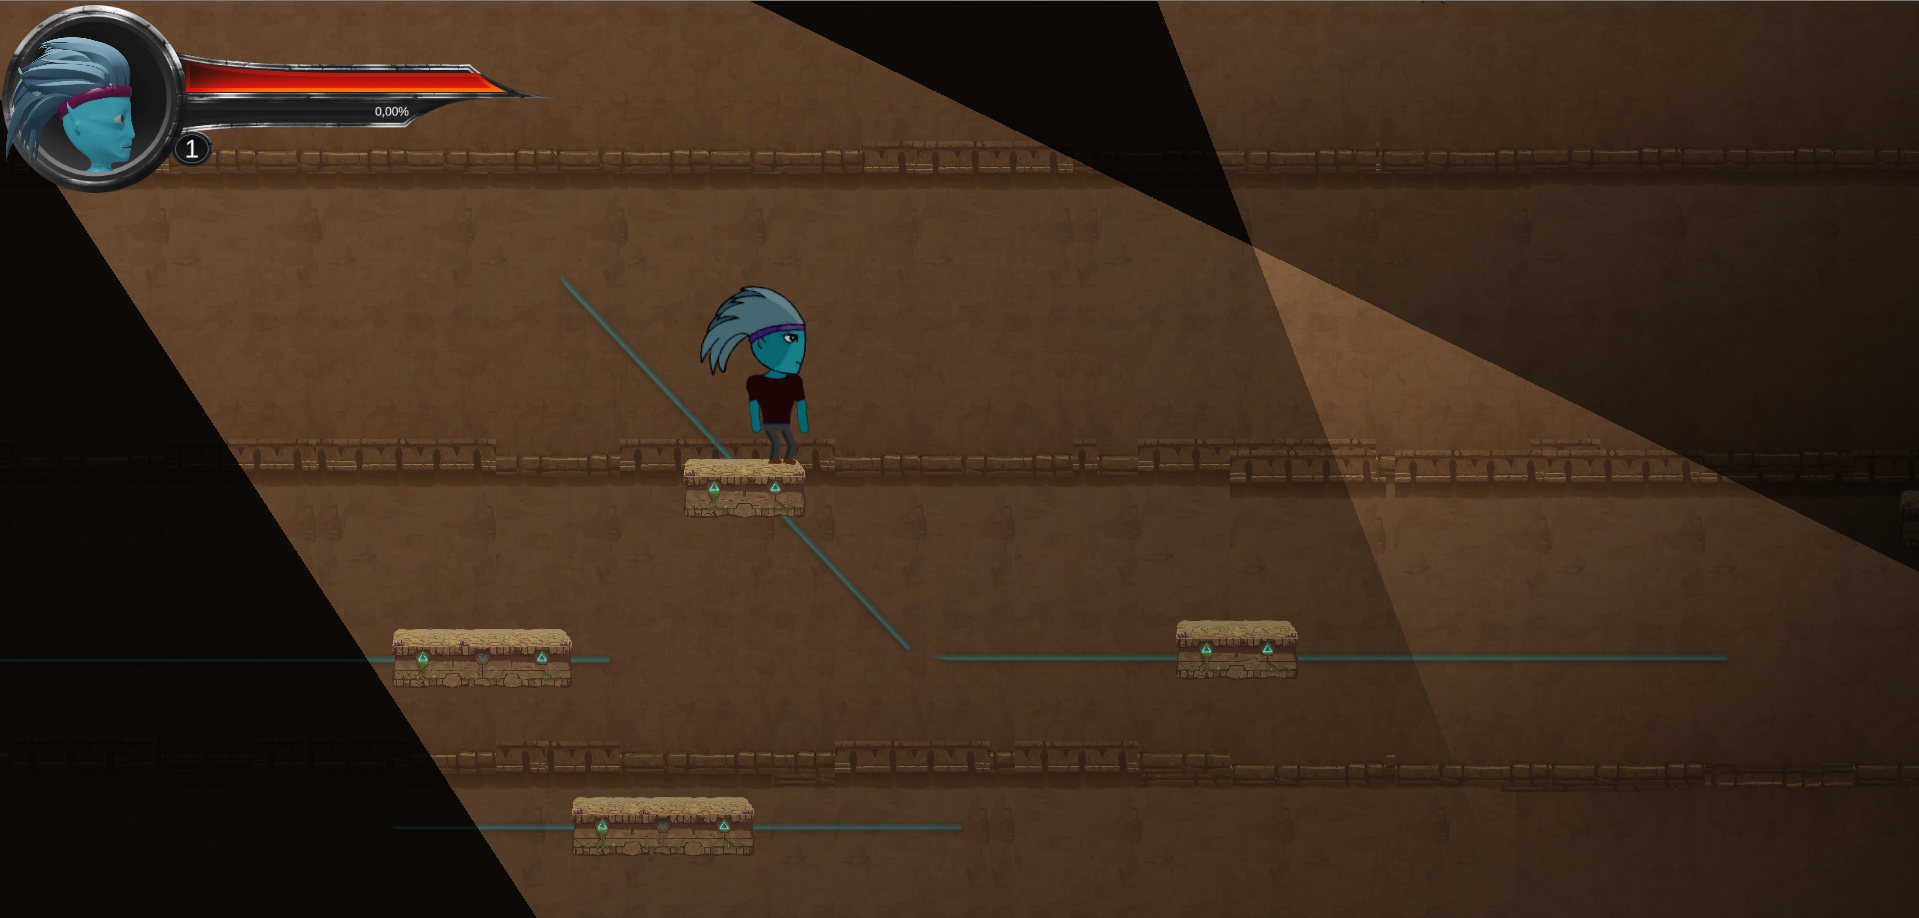
\includegraphics[width=13cm]{images/hyps/platfAfter.png}
	\caption{Ostatnia iteracja ruchomych platform. Przykład z~,,The Lore''}
\end{figure}

Był to tylko jeden z~wielu procesów poprawionych dzięki otrzymanej opinii podczas testów, jednak wystarczająco poważny, by pokazać, jak kluczowym dla projektu „The Lore” było wybranie metodyki Agile.
\newpage
\section{Podsumowanie}
W~niniejszym rozdziale pracy zostały przedstawione fundamentalne pojęcia oraz procesy realizacji projektu informatycznego. Poprzez zdefiniowanie i~zobrazowanie podstawowego podziału cyklu życia projektu oraz wskazanie kilku najważniejszych i~najpopularniejszych zagadnień poszczególnych elementów – przybliżono życie projektu. Dzięki długiemu wprowadzeniu możliwe było przedstawienie owego procesu na przykładzie gry „The Lore”. Podkreślając wagę każdego członu projektu, można zauważyć, jak niezbędną rolę ma cały proces i~każdy jego element, który pozwala z~wyższym prawdopodobieństwem ukończyć projekt z~sukcesem.

\chapter{Zagadki logiczne}
\section{Wprowadzenie do zagadek logicznych}
\subsection{Omówienie zagadnienia}
\par Zagadką logiczną określamy zadanie, którego celem jest odnalezienie odpowiedzi na pytanie, logiczne dojście do rozwiązania problemu, czy też czasami abstrakcyjne myślenie. Możemy wyróżnić różne rodzaje zagadek, między innymi graficzne, czego przykładem jest znany, często używany w~szkołach podstawowych rebus. Główną ideą takiej rozgrywki jest rozwój swoich intelektualnych możliwości przy dobrej zabawie. \cite{zagadka_logiczna}

\subsection{Przykłady logicznych zagadek w~prawdziwym świecie}
\subsubsection{Rebus}
\par Jednym z~przykładów takiej zagadki może być rebus. To prosta rozgrywka, polegająca na odgadnięciu hasła na podstawie przytoczonego obrazka. Często treści w~rebusach mogą być niejednoznaczne, co sprawia, iż nie są one trywialne i~wymagają wielu kombinacji haseł, związanych z~danym obrazkiem. \cite{rebus}

\begin{figure}[h]
\centering
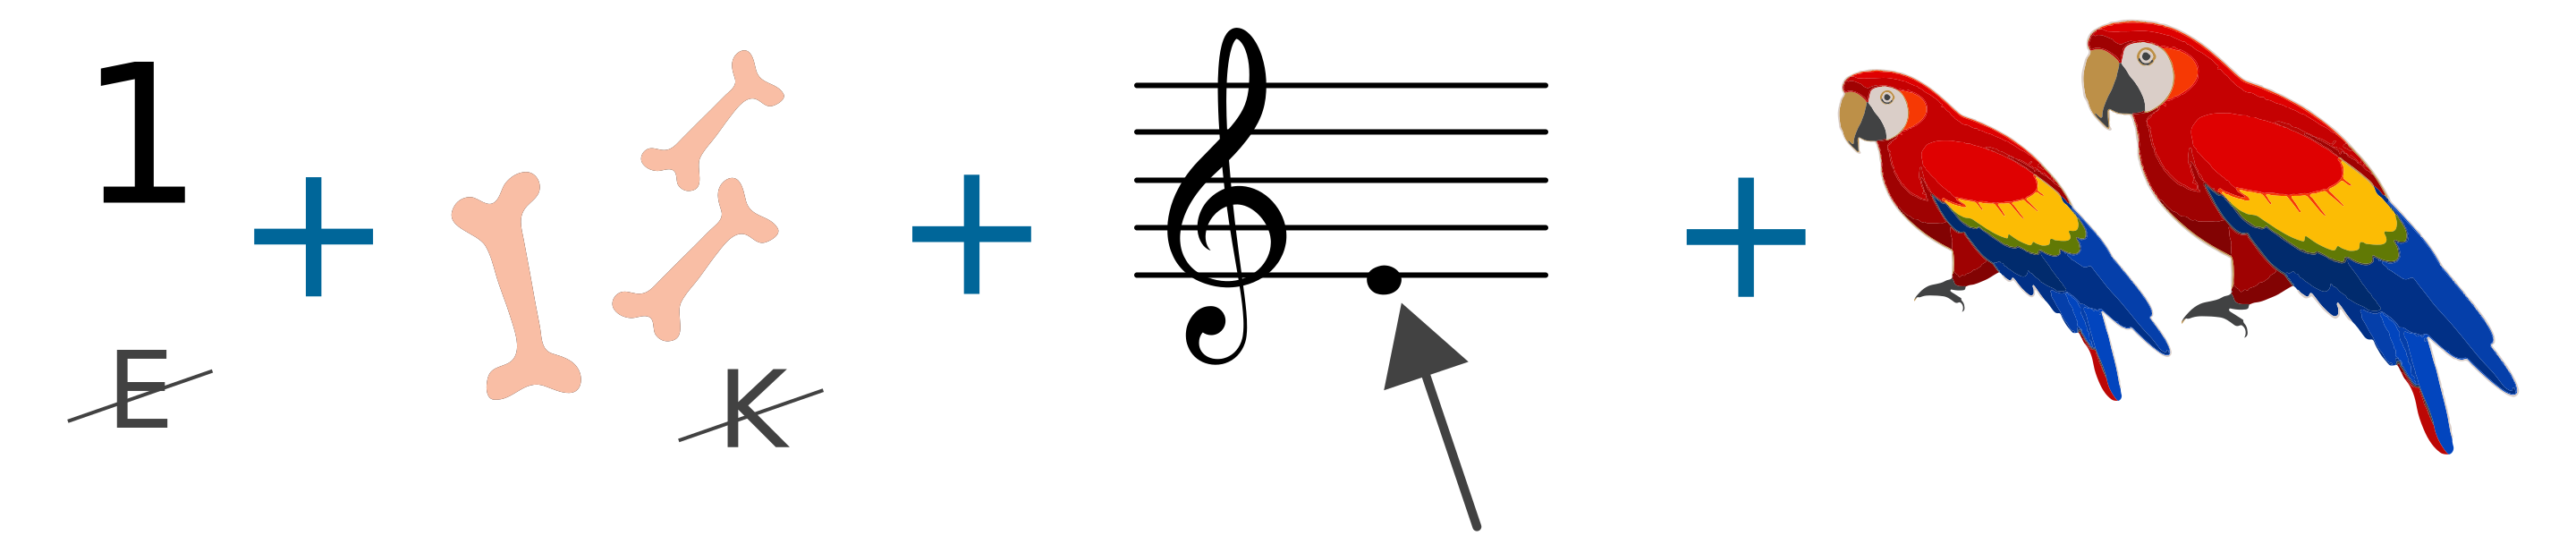
\includegraphics[width=8cm]{images/tyrek/rebus.png}
\caption{Rebus. Źródło: Zespół autorski Politechniki Łódzkiej, licencja: CC BY 3.0}
\end{figure}

\subsubsection{Piętnastka – przesuwane puzzle}
\par Kolejnym przykładem może być też piętnastka, która w~grze ,,The Lore'' została zaimplementowana jako przesuwane puzzle rozmiarów 3 na 3. Temat ten szerzej poruszony będzie w~dalszej części pracy, gdzie oprócz założeń związanych z~rozwiązaniem zagadki, przedstawiona zostanie logika idąca za zrealizowaniem tej zagadki w~grze opartej na silniku Unity. 

\begin{figure}[h]
\centering
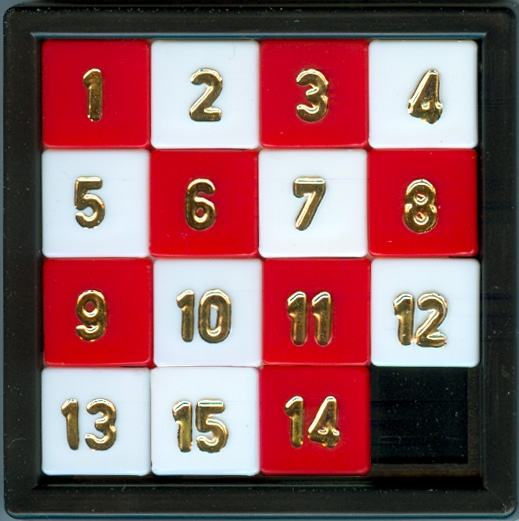
\includegraphics[width=5cm]{images/tyrek/przesuwane-puzzle.jpg}
\caption{Piętnastka. Źródło: Wikipedia, Sliding Puzzle, Micha L. Rieser – Public Domain}
\end{figure}

\subsubsection{Puzzle}
\par Jedną z~najpopularniejszych zagadek logicznych są puzzle. Jest to gra, w~czasie której rozwiązujemy problem polegający na ułożeniu z~dostępnych elementów logicznego obrazka, który zazwyczaj jest dołączony do gry – w~postaci fotografii umieszczonej w~zestawie lub na pudełku.
Słowo ,,puzzle'' pochodzące z~XVI wieku, oznaczało ,,stan zagubienia''. Sama gra ma swoje początki w~wieku XVIII, gdy John Spilsbury, grawer i~kartograf umieścił mapę na drewnie, następnie przepiłował ją wokół konturów każdego kraju, który się na niej znajdował. To co powstało postanowił użyć do nauki geografii – ułożenie logicznej mapy uczyło jak wygląda mapa danego regionu. Taka pomoc dydaktyczna zdobyła szybko popularność, wszak była to nauka przez zabawę, stosowano ją dość często, nawet jeszcze w~wieku XIX.  
Trudność puzzli zależy zazwyczaj od kształtu elementów i~ich ilości. Puzzle często mają specyficzny kształt, przez co nie każdy element pasuje do innego, co pozwala nam odrzucić możliwość połączenia niektórych par. Ilość elementów zwiększa ilość możliwych oraz logicznych kombinacji danych puzzli, przez co zwiększa się czas realizacji zadania. Największa układanka została wykonana przez firmę Educa, posiadała ona aż 42 000 elementów i~przedstawia dość bajeczny krajobraz, na którym znajdują się najpopularniejsze budynki z~całego świata – Big Ben, wieża Eiffla czy Krzywa Wieża w~Pizie. Ułożenie tej układanki możemy liczyć w~setkach godzin. \cite{puzzle}

\begin{figure}[h]
\centering
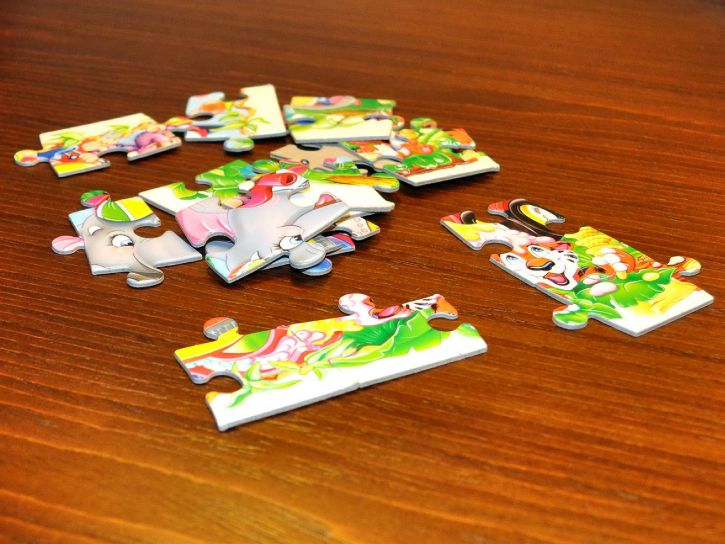
\includegraphics[width=5cm]{images/tyrek/puzzle.jpg}
\caption{Źródło: Pixnio, Przykład puzzli – Public Domain}
\end{figure}

\subsection{Wdrożenie zagadek do gry opartej na silniku Unity}
\par Zanim przedstawione zostaną dwa sposoby wdrażania zagadek, ze względu na sposób umieszczenia mini-gry w~odpowiedniej hierarchii projektowej, warto poznać podstawowe pojęcia, które dotyczą projektu Unity.

\subsubsection{Scena w~Unity}
\par W~Unity możemy podzielić naszą grę na sceny. Scena to obiekt zawierający nasze menu, czy dane środowisko gry (na przykład poziom gry). Dobrą praktyką jest, aby każdy level gry był osobną sceną, co skróci czas jego ładowania. W~scenie możemy umieścić swoje obiekty, skrypty czy grafiki. \cite{scena}

\subsubsection{Obiekt – GameObject}
\label{sec:gameobject}
\par Obiekt, zwany w~Unity GameObject, to klasa podstawowa dla wszystkich podmiotów w~scenach Unity. Do każdego obiektu możemy przypinać kolejne obiekty, tworząc hierarchiczność, która może się przydać w~odpowiedniej realizacji projektu. \cite{gameobject}

\begin{figure}[h]
\centering
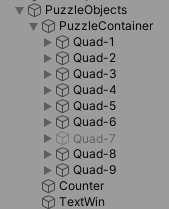
\includegraphics[width=4cm]{images/tyrek/hierarchia.png}
\caption{Hierarchia obiektów. Przykład z~projektu ,,The Lore''}
\end{figure}

\subsubsection{Komponent}
\label{sec:komponent}
\par Komponent jest klasą podstawową dla GameObject. Jest to klasa, przykładowo w~języku C\#, która dołączana jest do obiektu Unity, celem wykonania na nim jakichś operacji. \cite{komponent}
\subsubsection{Sposoby dodawania mini-gier}
\par W~toku pracy nad projektem ,,The Lore'' rozpatrywano dwa sposoby dodawania mini-gier do gry:
\begin{itemize}
\item{Każda mini-gra jest w~osobnej scenie:}
\begin{itemize}
\item w~przypadku rozbudowanych poziomów nie powiela szerokiej listy obiektów sceny,
\item Pozwala na mniejsze pobieranie zasobów w~danej jednostce czasu – połączenie działającego poziomu z~algorytmiką mini-gry, może bywać uciążliwe na słabszych komputerach.
\end{itemize}
\item{Każda mini-gra zawiera się w~scenie poziomu gry:}
\begin{itemize}
\item Unikamy dłuższego ładowania się poziomu gry po zakończeniu mini-gry.
\end{itemize}
\end{itemize}
Po wewnętrznej dyskusji wybrano opcję wydzielenia do osobnej sceny. W~toku testowania tego rozwiązania uznano, iż nie jest ono bardzo uciążliwe pod kątem czasu ładowania poziomu, natomiast pozwala na zachowanie porządku w~projekcie. Jak się okazało już w~przypadku tworzenia poziomu pierwszego gry, ta decyzja była właściwa. Z~racji sporego rozbudowania tej sceny i~dużej liczby obiektów na niej zawartych, dodanie mini-gier do tej sceny mogłoby spowodować chaos organizacyjny. Dodatkowo mogłoby wydłużyć czas ładowania poziomu i~spowodować pobieranie większych zasobów w~czasie gry.


\section{Przesuwane puzzle}
\subsection{Omówienie zagadnienia i~ogólne założenia}
\par Przesuwane puzzle to układanka, złożona zazwyczaj z~kwadratowej liczby elementów, najczęściej jest to szesnaście pól. Pola są jednakowych rozmiarów i~oznaczone są liczbami od 1 do (\(n\)-1), gdzie \(n\) to liczba dostępnych pól w~układance. Jedno pole jest puste, pozwala to na przeniesienie sąsiednich elementów puzzli względem siebie. Rozgrywka kończy się, gdy ułożymy puzzle w~odpowiedniej kolejności, według rosnącego porządku liczb lub powstania odpowiedniego obrazka. Trudno określić kto odpowiada za stworzenie zagadki. Wiadome jest, że w~1878 roku pochodzący ze Stanów Zjednoczonych Samuel Loyd wypromował układankę, jednak prawdopodobnie nie jest to jego pomysł. Dość popularną nazwą na rozgrywkę jest ,,piętnastka'', określająca ilość dostępnych pól w~najpopularniejszym ułożeniu – 4 na 4.  \cite{przesuwane_puzzle}

W~grze ,,The Lore'' gracze staną przed rozwiązaniem zagadki, gdzie do dyspozycji mają dziewięć pól. Podczas projektowania układanki w~grze uznano, iż zagadka z~piętnastoma elementami może być dość trudna, a~korzyści płynące z~rozwiązania jej będą nieadekwatne do poświęconego czasu, stąd ilość pól jest mniejsza niż w~najpopularniejszej wersji rozgrywki.
\subsection{Algorytmika}
\subsubsection{Pojedynczy element puzzle – PuzzleBlock}

\par Każdy pojedynczy element puzzla jest tworzony jako obiekt, który określamy jako PuzzleBlock. Obiekt posiada koordynaty, które określają jego położenie w~przestrzeni na układance.

\begin{figure}[h]
\centering
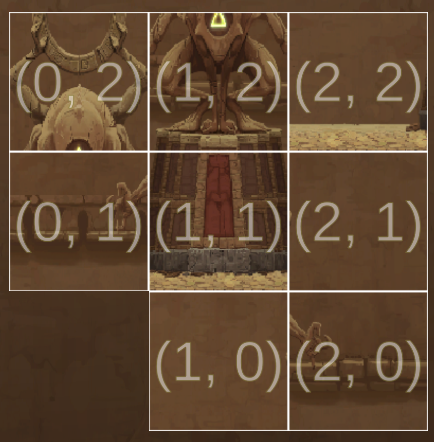
\includegraphics[width=6cm]{images/tyrek/coord_puzzle.png}
\caption{Koordynaty każdego pola. Przykład z~gry ,,The Lore''}
\end{figure}

Tak jak na załączonym przykładzie, wartość \(x\) rośnie w~prawą stronę, natomiast \(y\) w~górę, gdzie \(x\) dotyczy położenia w~poziomie, a~\(y\) w~pionie. W~założeniach przedstawiona została logika, która mówiła, iż element może zostać przemieszczony wtedy i~tylko wtedy, gdy pole obok niego jest wolne, czyli nie posiada żadnego PuzzleBlock – elementu z~liczbą lub obrazkiem. Dla lepszego efektu wizualnego, w~grze ,,The Lore'' element porusza się stopniowo, aby sprawiał wrażenie, iż porusza się realistycznie. Z~racji, iż w~Unity każda akcja wykonuje się podczas pokazywania kolejnej klatki, element porusza się w~minimalnym stopniu w~trakcie jednej klatki. 

\subsubsection{Plansza – Puzzle. Losowanie kolejności puzzli}
\par Plansza rozgrywki posiada 8 elementów PuzzleBlock oraz jedno puste pole.  Algorytm powinien wylosować dla 8 pól ich położenie na planszy – tak jak w~wyżej przedstawionym przykładzie. W~tym celu na początku należy wylosować dla każdego bloku wartość od 0 do 8. W~C\# można to zrobić przy użyciu funkcji  \emph{System.Random().Next(a, b)}, który losuje wartości z~zakresu \(<a, b)\). Przykładowo:
\begin{lstlisting}[
language={[Sharp]C},
rulecolor=\color{blue!80!black},
caption={Fragment klasy \texttt{Puzzle.cs}}
]
private int randomPosition()
{
    int pos = 0;
    do
    {
        pos = new System.Random().Next(0, 9);
    }
    while (isOnBoard[pos]);
    isOnBoard[pos] = true;
    return pos;
}
\end{lstlisting}

Gdzie \texttt{isOnBoard[pos]} jest tablicą, która weryfikuje, czy dane pole nie jest już zajęte. Jeśli jest, należy ponownie wylosować wartość dla PuzzleBlock. Oczywiście to nie koniec – z~tej wartości trzeba stworzyć położenie w~postaci (\(x\), \(y\)), gdzie \(x\) to położenie w~poziomie, a~\(y\) w~pionie. W~tym celu jedna z~tych wartości będzie resztą dzielenia wylosowanej pozycji przez trzy (ilość pól w~linii), a~druga ilorazem całkowitym pozycji i~liczby trzy. 
Kolejną ważną rzeczą będzie weryfikacja, czy obecne ułożenie puzzli jest wykonalne.

\subsubsection{Plansza – Puzzle. Weryfikacja kolejności puzzli}
\par Jak się okazuje niektóre ułożenia puzzli powodują, iż nie ma żadnego rozwiązania tego problemu. Z~taką sytuacją spotykaliśmy podczas pierwszych testów mini-gry puzzle. 
\begin{figure}[h]
	\centering
	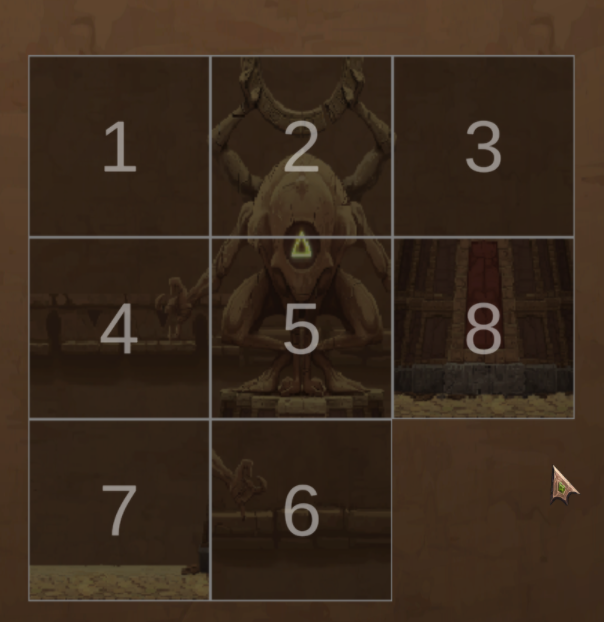
\includegraphics[width=5cm]{images/tyrek/puzzle_1.png}
	\caption{Puzzle bez rozwiązania. Przykład z~gry ,,The Lore''}
\end{figure}

Występuje tutaj dość prosta zasada. Łamigłówka przesuwanych puzzli z~8 elementami jest rozwiązywalna wtedy i~tylko wtedy, gdy liczba inwersji stanu początkowego jest parzysta. Czym jest zaś w~tym przypadku liczba inwersji?

Inwersją nazwiemy parę liczb, której wartości są w~odwrotnej kolejności, niż w~zakładanym stanie końcowym. \cite{solvablePuzzle}

\begin{center}
\begin{tabular}{ | m{5em} | m{1cm}| m{1cm} | } 
\hline
 1 & 2 & 3 \\ 
\hline
 6 & 4 & 5 \\
\hline  
 7 & 8 &     \\
\hline
\end{tabular}
\end{center}

W~tym przypadku liczba inwersji wynosi dwa. Elementami zbioru inwersji są pary (6,4) oraz (6,5) – jak wiadomo, liczba 6 jest w~kolejności po cyfrach 4 oraz 5. W~tym przypadku można rozwiązać puzzle.

\begin{center}
\begin{tabular}{ | m{5em} | m{1cm}| m{1cm} | } 
\hline
 1 & 2 & 3 \\ 
\hline
 6 & 5 & 4 \\  
\hline
 7 & 8 &     \\
\hline
\end{tabular}
\end{center}

W~tym przypadku liczba inwersji wynosi już trzy. Elementami zbioru są pary (6,5), (6,4) oraz (5,4). Takich puzzli nie da się rozwiązać. 
W~projekcie platformowej gry w~Unity zastosowaliśmy prostą weryfikację tej sytuacji. 
\\
\begin{lstlisting}[
language={[Sharp]C},
rulecolor=\color{blue!80!black},
caption={Fragment klasy \texttt{Puzzle.cs}}
]
int inversions = 0;
for (int i= 0; i< numbersOrdered.Length - 1; i++) {
    for (int j1 = i+ 1; j1 < numbersOrdered.Length - 1; j1++) {
        if (numbersOrdered[j1] > numbersOrdered[i]) {
            inversions++;
        }
    }
}

\end{lstlisting}
\par Gdzie \textbf{inversions}, to liczba znalezionych inwersji, a~\textbf{numberOrdered} to lista kolejności puzzli w~stanie wejściowym. Jeżeli wartość \(x\) znajduje się w~liście \textbf{numberOrdered} przed wartością \(y\) i~jest od niej większa, to wtedy licznik inwersji zwiększa się o~jeden.
Oczywiście pozostaje prosta weryfikacja, czy liczba inwersji jest nieparzysta – w~takim wypadku puzzle będą nierozwiązywalne.
\begin{lstlisting}[
	language={[Sharp]C},
	rulecolor=\color{blue!80!black},
	caption={Fragment klasy \texttt{Puzzle.cs}}
	]
	if (inversions % 2 == 1)
	{
	pab.restartPuzzleButton();
	}
\end{lstlisting}

Gdzie \textbf{pab} jest obiektem odwołującym się do akcji \textbf{PuzzleActionsButton}, zawierającym przycisk restartButton – ten sam, który dostępny jest w~grze w~celu zrestartowania obecnego ułożenia puzzli.

Każdy obiekt (puzzle) ma przypisane do siebie dwie akcje: \textbf{OnBlockPressed} i~\textbf{OnFinishedMoving}. Pierwsza akcja dotyczy tego, co ma się dziać, w~momencie wybrania przez gracza danego elementu. W~tym przypadku dany element dodawany jest do kolejki, której zadaniem jest kontrola poruszania się puzzli. Pozwala to uniknąć sytuacji, gdy użytkownik zdołałby w~bardzo szybkim czasie wybrać dwa elementy – wtedy użytkownicy mogliby być świadkami nachodzących się puzzli lub nawet wejścia dwóch elementów na jedno miejsce. Gdy element będzie pierwszy w~kolejce, rozpocznie się ruch naszego elementu – wtedy też przypisane będą mu nowe pozycje. Wtedy przychodzi czas na drugą akcję, \textbf{OnFinishedMoving}. Początkowo funkcja zwiększa ilość ruchów o~jeden. Następnie sprawdza, czy obecne ułożenie puzzli odpowiada oczekiwanemu wynikowi końcowemu. Jeśli tak, użytkownik informowany jest o~ilości zdobytego doświadczenia. Ponownie przedstawiana jest animacja przesuwającej się płytki, tym razem zamykającej się. Jeśli nie, algorytm sprawdza, czy istnieją elementy w~kolejce, w~tym przypadku powtarza się część procedury wykonywanej w~\textbf{OnBlockPressed} – element porusza się na swoje miejsce, zmieniając koordynaty, następnie znów wykonując akcję \textbf{OnFinishedMoving}.

\subsection{Przedstawienie przykładu w~grze ,,The Lore''}
\par W~grze ,,The Lore'' zagadka przesuwanych puzzli pełni rolę opcjonalnej rozgrywki, a~za jej rozwiązanie gracz otrzymuje punkty doświadczenia. Mini-grę możemy rozpocząć, znajdując się w~pobliżu charakterystycznej płytki, wyróżniającej się podświetleniem.\begin{figure}[h]
	\centering
	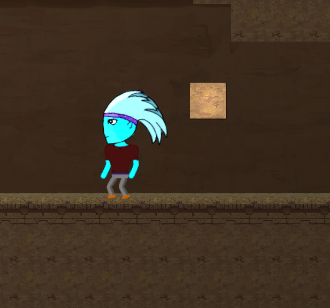
\includegraphics[width=6cm]{images/tyrek/the_lore_puzzle_lvl1.png}
	\caption{Miejsce rozpoczęcia puzzli. Przykład z~projektu ,,The Lore''}
\end{figure}

W~momencie naciśnięcia przycisku akcji kamera zbliża się do obiektu, czyli podświetlonej płytki. Następnie widzimy animację otwierającej się płytki sprawiającej wrażenie, iż ścianka jest przesuwana przez gracza.
\begin{figure}[h]
	\centering
	\includegraphics[width=7cm]{images/tyrek/otwieraniePuzzli.png}
	\caption{Animacja rozpoczęcia puzzli. Przykład z~projektu ,,The Lore''}
\end{figure}

Po skończonej animacji rozpoczynamy mini-grę. Oprócz bloczków z~kolejnością, na ekranie widzimy również dwa przyciski i~cyfrę zero.
\begin{figure}[h]
	\centering
	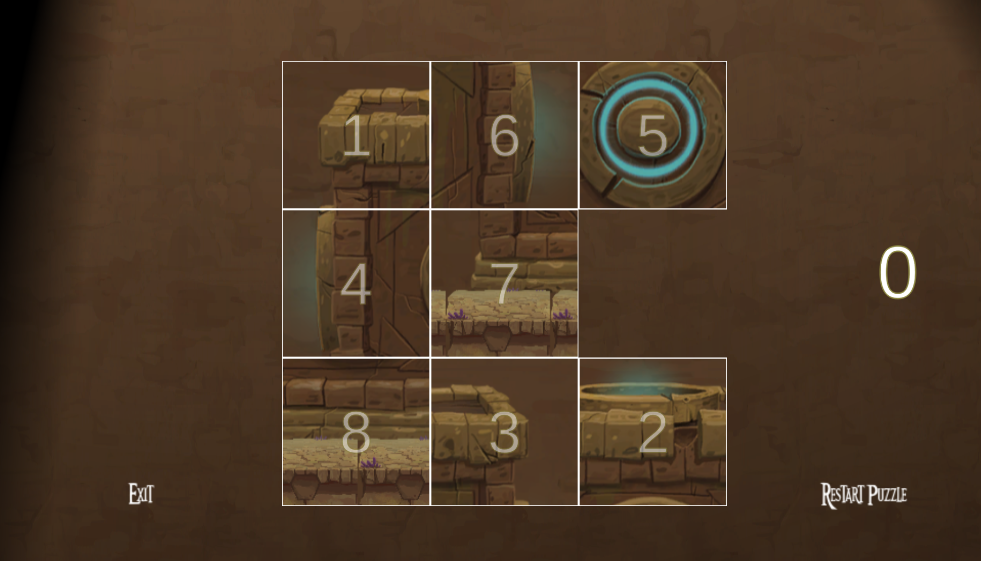
\includegraphics[width=7cm]{images/tyrek/puzzlebuttons.png}
	\caption{Cały interfejs mini-gry puzzle. Przykład z~gry ,,The Lore''}
\end{figure}

Gdzie \textbf{Exit} kończy rozgrywkę, przenosząc nas z~powrotem w~miejsce, w~którym rozpoczynaliśmy zagadkę, \textbf{Restart Puzzle} powoduje ponowne rozlosowanie puzzli, odwołując się do akcji w~klasie \textbf{PuzzleActionsButtons}, czyli tej samej, która uruchamiana jest w~przypadku, gdy puzzle nie mają rozwiązania. Dodatkowo, po prawej stronie widnieje informacja, ile ruchów do tej pory wykonaliśmy, rozwiązując zagadkę. Jest to dość istotna informacja dla gracza, gdyż to od ilości ruchów zależy, ile punktów doświadczenia zdobędzie za rozwiązanie tej zagadki. Zastosowany wzór dla gry ,,The Lore'' wygląda następująco:

$$
y = \left\{ \begin{array}{ll}
5 & \textrm{gdy $x>=250$}\\
100 - (x / 25) * 10 & \textrm{gdy $x<250$}\\
\end{array} \right.
$$
Gdzie \(x\) jest liczbą wykonanych ruchów.
Po zakończeniu mini-gry gracz jest informowany o~ilości zdobytego doświadczenia.
\begin{figure}[h]
	\centering
	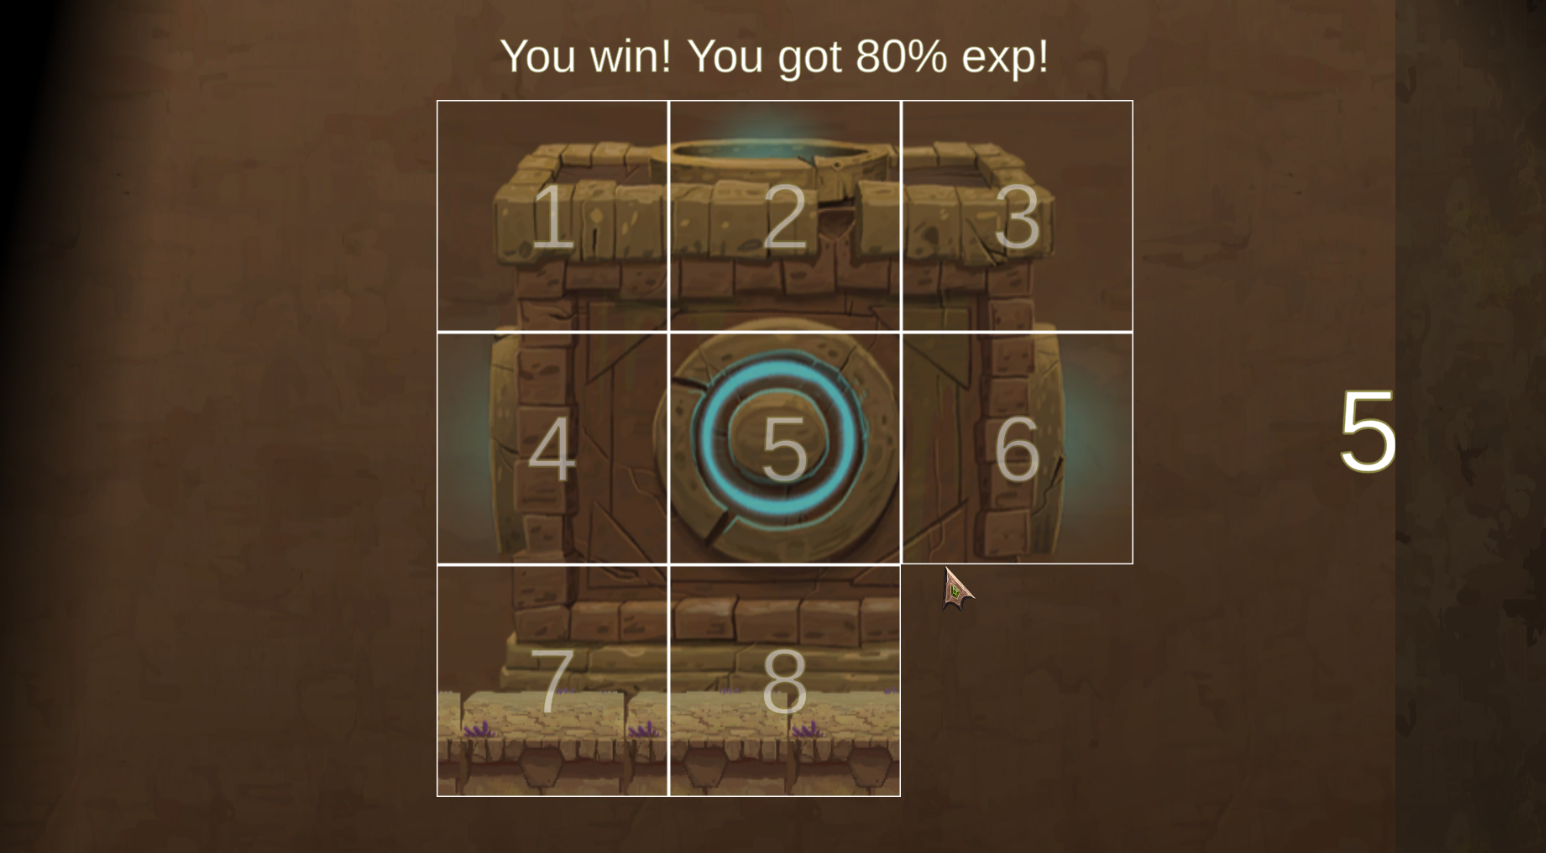
\includegraphics[width=7cm]{images/tyrek/puzzle_end.png}
	\caption{Wygrana rozgrywka puzzle. Przykład z~gry ,,The Lore''}
\end{figure}

Każdą mini-grę puzzle można wykonać w~grze tylko jeden raz. Ponowne próby są niemożliwe, a~o~tym, iż zagadka została zakończona, gracz informowany jest przez fakt, iż płytka symbolizująca mini-grę nie jest podświetlona.

\begin{figure}[h]
	\centering
	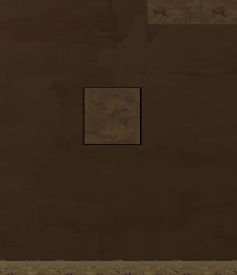
\includegraphics[width=5cm]{images/tyrek/puzzleWin.png}
	\caption{Wygaszona płytka. Przykład z~gry ,,The Lore''}
\end{figure}


\subsection{Przedstawienie przykładu w~innych grach}
\subsubsection{Nancy Drew: Hauting of Castle Malloy}
\par \emph ,,The Haunting of Castle Malloy'' to gra dwuwymiarowa, przygodowa, osadzona w~Irlandii. Postać wybiera się do tego kraju, aby zostać drużbą na ślubie swojego przyjaciela. Jadąc autem na uroczystość, zostaje zaatakowany przez upiorną postać, przez co wpada do rowu. Jak się później okazuje, zaginął Pan Młody. Główny bohater, Nancy Drew chce odkryć tajemnicę, przechodząc przez świat pełny zagadek. Właśnie podczas poszukiwania swojego Pana Młodego, gracz natyka się na przesuwane puzzle. 
\begin{figure}[h]
	\centering
	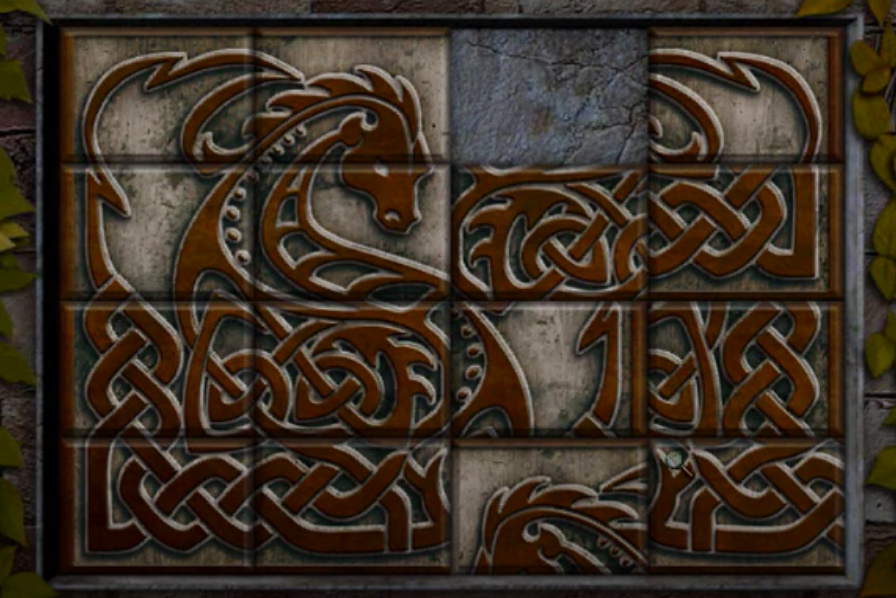
\includegraphics[width=6cm]{images/tyrek/nd.png}
	\caption{Przesuwane puzzle. Przykład z~gry ,,Nancy Drew: Hauting of Castle Malloy''}
\end{figure}

W~czasie przechodzenia kolejnych etapów użytkownik ma możliwość przyglądania się obiektom, które mija. To właśnie w~tym momencie może natrafić na omawianą rozgrywkę. Przed mini-grą gracz widzi, jaki jest stan wyjściowy puzzli. Co warto podkreślić, w~przeciwieństwie do gry ,,The Lore'', na poszczególnych elementach puzzli nie widzimy cyfr oznaczających poprawną kolejność puzzli. Aby zakończyć zagadkę, należy również posiadać ostatni element, który po ułożeniu obrazka umieszczamy w~brakującym miejscu. \cite{nd}


\subsubsection{Resident Evil 4}
\par ,,Resident Evil 4'' jest grą typu survival horror. Toczy się ona w~fikcyjnym mieście Raccoon City, gdzie po sześciu latach kończy się śledztwo dotyczące nielegalnych badań i~eksperymentów medycznych nad wirusem, prowadzone przez organizację Umbrella. Działania firmy spowodowały destabilizację tego miasta. Główny bohater, Leon S. Kennedy zostaje wyznaczony jako agent, który ma odnaleźć porwaną przez podejrzaną organizację, córkę prezydenta USA. Bohater, przemierzając kolejne miasta, odkrywa tajemnice związane z~porwaniem. W~toku gry zdarza się, iż gracz kieruje Ashley Graham, czyli porwaną córką prezydenta USA. To właśnie w~czasie kontrolowania tej postaci możemy natrafić na mini-grę związaną z~przesuwanym puzzlami. Bohaterka może natrafić na totem, gdzie widać osiem elementów. Dialogi bohaterki podpowiadają graczowi, iż elementy mogą ułożyć się w~logiczną całość. W~przeciwieństwie do poprzedniego przykładu nie mamy tutaj pokazanego oczekiwanego ułożenia planszy. Ostatni element, tak jak w~,,Nancy Drew: Hauting of Castle Malloy'' musimy odnaleźć, aby zagadka została ukończona.

\begin{figure}[h]
	\centering
	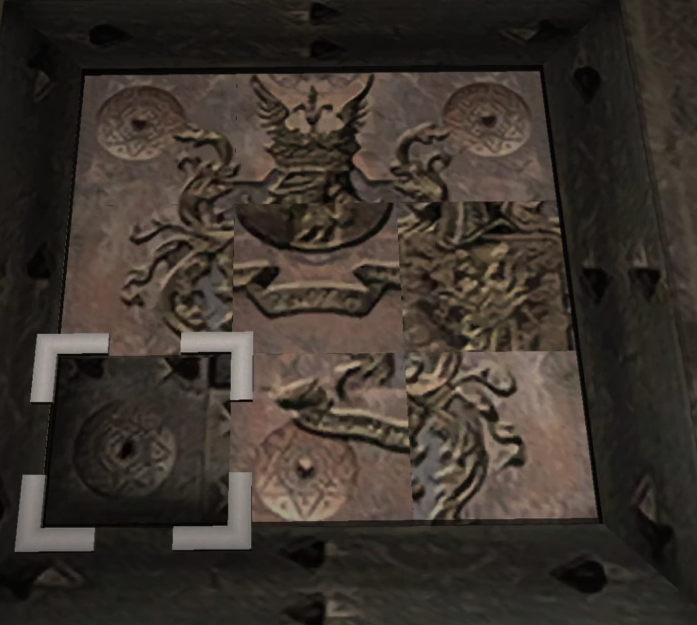
\includegraphics[width=5cm]{images/tyrek/re4.png}
	\caption{Przesuwane puzzle. Przykład z~gry ,,Resident Evil 4''}
\end{figure}


\section{Zagadka z~rurami}
\subsection{Omówienie zagadnienia}
\par Zagadka z~rurami jest rozgrywką, której celem jest ułożenie ścieżki z~dostępnych kształtów rur. Rodzaj rur jest tutaj ważny, ponieważ oprócz kształtów pionowych czy poziomych, dostępne są inne rodzaje – skośne, skrętne, półokrągłe.
Ścieżka powinna wyznaczać drogę wody, począwszy od źródła, zazwyczaj zaznaczonego niebieskim kolorem, do końcowej rury. Rozgrywka kończy się, gdy woda dotrze do ostatniej rury w~ścieżce, jeżeli będzie miejsce, w~którym powinna kończyć się droga, gracz wygrywa. W~innym wypadku ponosi porażkę.
Poziom naładowania wody pełni rolę wyznacznika czasu, w~którym użytkownik musi ułożyć odpowiednią ścieżkę. Zazwyczaj w~tego typu rozgrywkach, po pewnym czasie woda przenosi się z~rury źródłowej do kolejnej, aby dać graczowi pewien zapas czasowy na podjęcie odpowiednich decyzji. W~niektórych grach gracz ma wybór rur, które dostępne są przez całą rozgrywkę – tak jest przykładowo w~grze ,,The Lore''. Jednak są też cięższe przypadki, gdy mamy kolejkę kilku rur – wtedy musimy podejmować decyzję w~oparciu o~mniejszą pulę elementów.
\subsection{Algorytmika}
\par Mini-gra z~rurami jest dość złożoną rozgrywką, dlatego, zanim przedstawiony zostanie cały algorytm, warto na początku przytoczyć wszystkie obiekty, które pojawią się w~czasie przedstawienia procedury.
\subsubsection{Pipe}
\par Jest to obiekt związany z~rurą. To w~tym miejscu określany jest typ rury, nadawana jest mu grafika oraz nazwa – ostatni element związany jest wyłącznie z~częścią deweloperską, nie jest dostępne dla wszystkich użytkowników. W~grze ,,The Lore'' mamy dostępne kilka typów rur:
\begin{itemize}
  \item Rury pionowe – 9 elementów,
  \item Rury poziome – 4 elementy,
  \item Rury skrętne lewo-góra – 1 element,
  \item Rury skrętne prawo-dół – 2 elementy,
  \item Rury dół-lewo –  1 element,
  \item Rury dół-prawo – 2 elementy.
\end{itemize}
Jak wcześniej wspomniano, liczba elementów poszczególnych typów rur odgrywa ważną rolę. Nie jest możliwe ułożenie bez możliwości zejścia na dół (czyli między innymi bez rur skrętnych). 
\subsubsection{PipeSlot}
\par Jest miejscem, w~którym może znaleźć się obiekt typu \textbf{Pipe}. Plansza, na której możemy kłaść elementy, jest rozmiarów 8x5, czyli tworzonych jest czterdzieści instancji obiektu \textbf{PipeSlot}. Jeżeli na danym miejscu znajduje się obiekt \textbf{Pipe}, wtedy można wykonać na nim akcje – określa to zmienna \textbf{canDrag}. Do każdego obiektu przypisane są akcje \textbf{OnBeginDragEvent}, \textbf{OnEndDragEvent}, \textbf{OnDragEvent} oraz \textbf{OnDropEvent}. Związane są one ze systemem \textbf{Drag\&Drop} czyli przeciągania i~układania zadanych elementów. Jego działanie zostanie przedstawione w~dalszej części prezentowanej algorytmiki.
\subsubsection{Działanie algorytmu – UI}
\par Klasa \textbf{UI} odpowiada za interakcje z~widocznym interfejsem i~interakcje z~obiektami. Na samym początku, do każdego elementu \textbf{PipeSlot} przypisywane są jego akcje. Gdy to już się stanie, czyszczona jest lista \textbf{pipes} w~której trzymane będą wszystkie obiekty \textbf{Pipe}. Ma to na celu zabezpieczenie algorytmu przed wczytaniem elementów z~poprzedniej instancji rozgrywki. Następnie wszystkie obiekty \textbf{PipeSlot} jako obiekt \textbf{Pipe} nadany mają \emph{null} – również z~powodu zabezpieczenia przed niepożądanymi sytuacjami. Teraz czas na stworzenie dwóch najważniejszych \textbf{PipeSlot}, chodzi konkretnie o~pierwszy i~ostatni element. Dla tych miejsc przypisywana jest rura horyzontalna. Dodatkowo oba miejsca, pomimo iż znajduje się na nich rura, nie mogą być przeniesione – parametr \textbf{canDrag} ustawiony jest na \emph{false}. Oczywiście chodzi to o~nieingerowanie w~początek i~koniec algorytmu. Gdy to już się stanie, algorytm dodaje rury wszystkich typów do odpowiedniej tablicy – \textbf{pipes}. Dopiero wtedy następuje losowanie im miejsc. W~tym miejscu następuje przypisanie do elementu \textbf{PipeSlot} obiektów \textbf{Pipe}. Oczywiście, w~momencie losowania miejsc, procedura weryfikuje, czy na danym miejscu znajduje się już jakaś rura, dzieje się to w~dość trywialny sposób.

\begin{lstlisting}[
language={[Sharp]C},
rulecolor=\color{blue!80!black},
caption={Fragment klasy \texttt{UI.cs}}
]
if (pipeSlots[x].Pipe == null)
\end{lstlisting}
Jeżeli warunek nie jest spełniony, następuje ponownie losowane miejsca dla zadanego obiektu \textbf{Pipe}. Gdy warunek zostanie spełniony, rozpoczyna się rozgrywka. W~tym momencie zaczyna mijać czas, którego limit wyznacza zmienna \textbf{targetTime} – ustawiona na pięć sekund. Czas ten dotyczy przepływu wody przez jedną rurę. Co warto podkreślić, co każdą pełną sekundę zmienia się grafika danego obiektu \textbf{Pipe} – nadając efekt płynięcia wody.

\begin{figure}[h]
	\centering
	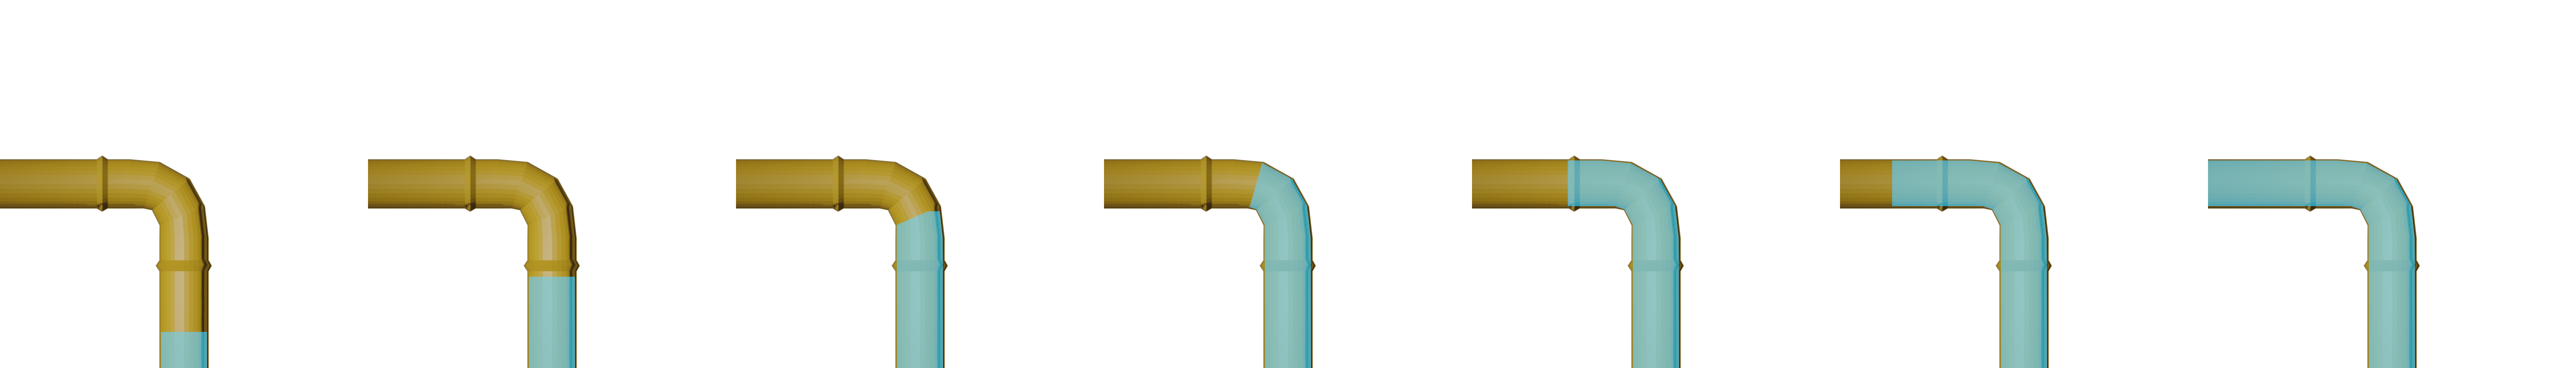
\includegraphics[width=10cm]{images/tyrek/rury-5.png}
	\caption{Grafiki rury skrętnej. Przykład z~projektu ,,The Lore''}
\end{figure}
W~danym momencie procedura weryfikuje też, czy istnieje połączenie. Dzieje się to poprzez warunki:
\begin{lstlisting}[
language={[Sharp]C},
rulecolor=\color{blue!80!black},
caption={Fragment klasy \texttt{UI.cs}}
]
if (recentPipe.right && (i+ 1) % 8 != 7 
&& pipeSlots[i + 1].Pipe.left 
&& !cameFrom.Equals("right"))
\end{lstlisting}
Gdzie \textbf{recentPipe.right} to sprawdzanie, czy obecna rura może skręcić w~prawo, \textbf{((i~+ 1) \% 8 != 7)} jest weryfikacją, czy rura znajduje się przy najbardziej wysuniętym na prawo \textbf{PipeSlot}. Następnie należy zweryfikować, czy sąsiedni slot może być skrętny w~lewo. Podobnie należy sprawdzić to dla wszystkich stron, z~odpowiednimi wartościami dla danych przypadków. Jeżeli minie czas, a~dany \textbf{PipeSlot} nie będzie miał odpowiedniego połączenia, użytkownik jest informowany o~porażce. Jeżeli zaś algorytm wykryje, iż takie połączenie istnieje, a~naszym obecnym indeksem na planszy jest 39 (liczba pól – 1), to algorytm przenosi gracza do poziomu gry, z~którego rozpoczął rozgrywkę.

\subsubsection{GameManager}
\par Ostatnim ważnym obiektem w~kontekście tej mini-gry jest GameManager. Odpowiada on za wszystkie akcje przypisane do \textbf{PipeSlot}. \textbf{BeginDrag}, \textbf{EndDrag} oraz \textbf{Drag} odpowiadają za przenoszenie danej rury – w~tym momencie pozycja obiektu jest ściśle związana z~kursorem na ekranie. W~momencie, gdy gracz puści lewy przycisk myszy, wykonuje się akcja \textbf{Drop}. Tutaj następuje weryfikacja, czy \textbf{Pipe} został przeniesiony na \textbf{PipeSlot}, który nie posiada żadnej rury. Jeśli tak, do danego miejsca przypisana jest nowa rura. W~innym wypadku rura wraca na swoje poprzednie miejsce. 
\subsection{Przedstawienie przykładu w~grze ,,The Lore''}
\par Jest to kolejna mini-gra zawarta w~grze ,,The Lore'', która jest elementem obowiązkowym do ukończenia poziomu ,,0'', odgrywającego rolę samouczka. Gracz, zbliżając się do miejsca, w~którym może rozpocząć rozgrywkę, informowany jest poprzez komunikat o~możliwości jej aktywacji.

\begin{figure}[h]
	\centering
	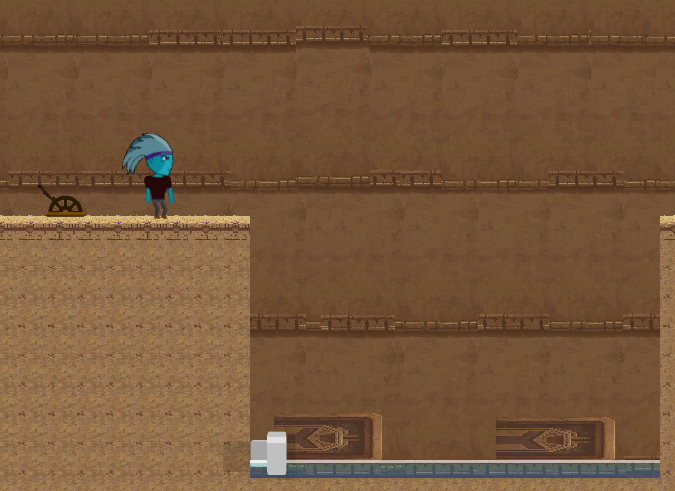
\includegraphics[width=7cm]{images/tyrek/ruryLvl0.png}
	\caption{Poziom 0 – Zagadka z~rurami. Przykład z~projektu ,,The Lore''}
\end{figure}

Jak widać na załączonym przykładzie, po prawej stronie znajduje się dół, w~którym widoczne są dwa totemy oraz płytki strumień wody. W~przypadku, gdyby gracz postanowił wskoczyć do dziury, zostanie przeniesiony z~powrotem w~okolice przełącznika (widocznego na fotografii po lewej stronie). Gdy gracz aktywuje przełącznik przyciskiem akcji, kamera zmierza w~dół, aby pokazać układ rur.

\begin{figure}[h]
	\centering
	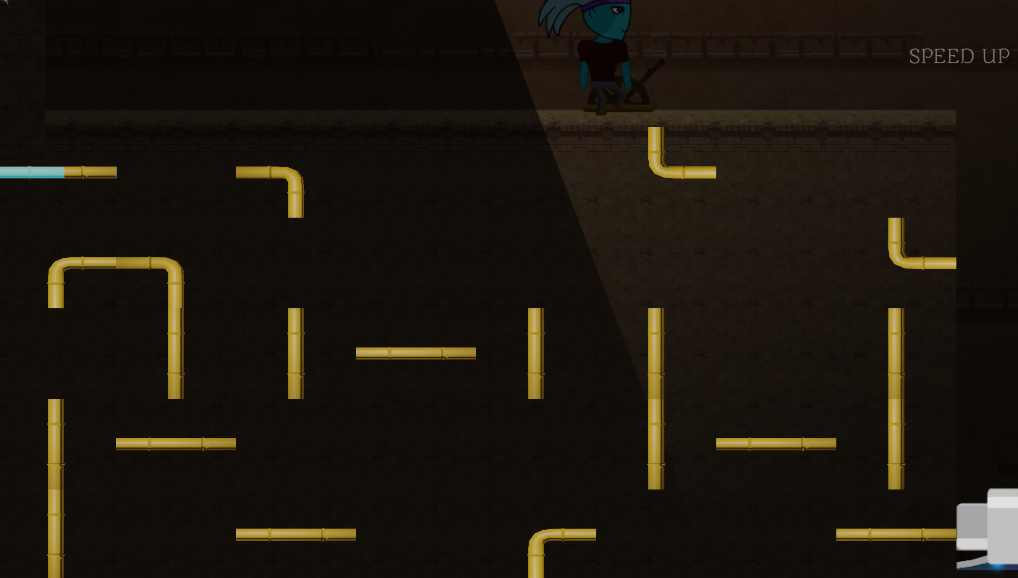
\includegraphics[width=12cm]{images/tyrek/pipes.png}
	\caption{Zagadka z~rurami. Przykład z~projektu ,,The Lore''}
\end{figure}

W~lewym górnym rogu widoczne jest źródło strumienia, zaś w~prawym dolnym rogu zakończenie (szara rura). Użytkownik, sterując myszką, może przekładać rury o~wybranym kształcie, tworzyć połączenia, celem stworzenia ścieżki, która jest konieczna do ukończenia mini-gry. Rozrywka zawsze generuje tę samą liczbę poszczególnych typów rur. Co warto podkreślić, liczba ta jest ważna – jeżeli dostępnych jest zbyt mało elementów danego typu, to po prostu ułożenie ścieżki może być niemożliwe. Zbyt duża liczba elementów zaś pozwoliłaby na trywialne rozwiązanie, na przykład w~kształcie litery L. W~grze ,,The Lore'' jest możliwość szybkiego zakończenia rozgrywki poprzez wybranie opcji \textbf{Speed Up}. Powoduje ona szybkie przeniesienie strumienia wody, do końcowej rury ułożonej przez nas ścieżki. Jeżeli odpowiednia droga została ułożona, mini-gra zostanie zakończona sukcesem, w~przeciwnym przypadku porażką.
\subsection{Przedstawienie przykładu w~innych grach}
\subsubsection{Pipe Mania}
\par Gra logiczna stworzona przez \emph{The Assembly Line} na platformy Amiga. Gra pojawiła się również na komputerach z~systemem Windows. Rozgrywka polega na ułożeniu rurociągu z~losowej puli rur. Kolejka rur, które otrzyma gracz, wyświetla się po lewej stronie ekranu. Cała gra polega na ułożeniu ścieżki z~dostępnych elementów, przy użyciu wszystkich rur. Liczba rur, które pozostały graczowi w~kolejce wyświetlona jest w~górnej części ekranu. Podobnie jak w~grze ,,The Lore'', woda rozpoczyna swój bieg po pewnym czasie, gracz widzi ten czas w~postaci paska po prawej stronie ekranu. \cite{pipemania}

\subsubsection{Soda Pipes}
\par Grą wzorowaną na poprzednim przykładzie jest ,,Soda Pipes''. Podobnie jak w~poprzedniej grze, gracz musi ułożyć ścieżkę z~rur, które losuje nam gra. W~odróżnieniu od poprzedniczki naszym celem jest zakończenie ścieżki w~danym miejscu. Gra oprócz typowej rozgrywki oferuje również tryby gry, takie jak "puzzle mode" – pozwala on na układanie rur bez ograniczenia czasowego oraz trybu, w~którym do pokonania jest 28 poziomów, które posiadają różne zadania. \cite{sp}

\section{Zagadka z~otwieraniem zamku}
\subsection{Omówienie zagadnienia}
\par Jest to bardzo powszechna mini-gra dodawana jest do wielu gier, które posiadają funkcjonalność posiadania ekwipunku. Jej celem jest otworzenie skrzyni, polega to na wykonaniu różnych operacji. Zazwyczaj zaczyna się od okrycia odpowiedniej sekwencji poruszania wytrychem, otwieranie zapadki poprzez poruszanie myszką, czy wciśnięcie odpowiedniego guzika, gdy postęp otwierania zamku jest na odpowiednim etapie. Otwarcie zamku pozwala graczom odblokować skrzynię, która zawiera elementy wyposażenia lub pozwala na otwarcie drzwi, które zaprowadzą nas do ważnych dla gry pomieszczeń. Z~racji na charakter rozgrywki element ten bywa raczej opcjonalną metodą przejścia gry. Z~tego względu w~niektórych grach, posiadających system umiejętności, otwarcie niektórych zamków jest niemożliwe lub bardzo trudne, jeżeli nie rozwiniemy odpowiednich umiejętności.
\subsection{Algorytmika}
\par Pierwszym i~najważniejszym dla całej mini-gry elementem jest wylosowanie przez grę sekwencji ruchów, która potrzebna jest do ukończenia rozgrywki. Odbywa się to w~skrypcie \textbf{PickLockGenerateSequence}. Podczas projektowania generatora napotkano problem związany z~ciągłym losowaniem tych samych liczb. Powodem jest tutaj oczywiście synchronizacja, która przy ładowaniu scen potrafi sprawiać deweloperom problemy. Z~tego powodu powstał ten skrypt, który wyróżnia się weryfikacją unikalności wylosowanej liczby.
Wszystko rozpoczyna się od losowania liczby z~zakresu <1,100).
\begin{lstlisting}[
language={[Sharp]C},
rulecolor=\color{blue!80!black},
caption={Fragment skryptu \texttt{PickLockGenerateSequence.cs}}
]
    private int randomSide()
    {
        int random = 0;
        do
        {
            random = new System.Random().Next(1, 100);
        } while (wasRandomed[random - 1]);
        wasRandomed[random - 1] = true;
        return random % 2;
    }
\end{lstlisting}
Tablica \textbf{wasRandomed} to element, który tworzony jest z~samych wartości \textbf{false}. Ilość elementów jest równa \textbf{n}, czyli ilości możliwych wylosowanych liczb. Jeżeli liczba zostanie wylosowana ponownie, skrypt próbuje wylosować kolejną. Tak jak wspominano, gracz ma dwie możliwości ruchów, dlatego, aby wszystko działało poprawnie, funkcja zwraca \textbf{mod 2} z~wylosowanego elementu. Wynikiem funkcji jest więc 0, co oznacza ruch w~lewo oraz 1, co oznacza ruch w~prawo. Losowanych jest pięć elementów, co tworzy tablicę ruchów, które musi wykonać gracz.

\begin{lstlisting}[
language={[Sharp]C},
rulecolor=\color{blue!80!black},
caption={Fragment skryptu \texttt{PickLockGenerateSequence.cs}}
]
for (int i = 0; i < numberOfMoves; i++)
{
   moves[i] = randomSide();
 }
\end{lstlisting}
Po wszystkim aktywowany jest \hyperref[sec:komponent]{\emph{komponent}} \textbf{Picklock}. Komponent ten odpowiada za wykrywanie jakich wyborów dokonał gracz. Jeżeli gracz wykonał dobry ruch, zostanie poinformowany o~tym poprzez komunikat oraz zwiększy się licznik kontrolny \textbf{step} ilości dobrych ruchów. W~przeciwnym razie licznik się wyzeruje. Dla efektu wizualnego gracz widzi, w~którą stronę poruszył się jego wytrych – pozwala to łatwiej zapamiętać wybór. Odbywa się to poprzez zmianę pozycji elementu \emph{transform}.

\begin{lstlisting}[
language={[Sharp]C},
rulecolor=\color{blue!80!black},
caption={Fragment skryptu \texttt{Picklock.cs}}
]
picklockTransform.position += 
new Vector3(10 * direction, 0, 0) * 0.1f;
\end{lstlisting}

Gdzie \textbf{picklockTransform} to \hyperref[sec:komponent]{\emph{komponent}} typu \emph{transform}, zawierający tablicę pozycji, rotacji oraz skalowania (odpowiednio parametry \emph{position}, \emph{rotation} i~\emph{scale}) \hyperref[sec:gameobject]{\emph{obiektu}}. W~tym przypadku ważny jest tylko \textbf{position}. 

\subsection{Przedstawienie przykładu w~grze ,,The Lore''}
W grze ,,The Lore'' otwieranie zamków dotyczy skrzyń, które położone są w~różnych częściach mapy. Podczas poziomu samouczka użytkownik informowany jest o~możliwości rozpoczęcia mini-gry. Rozpoczęcie mini-gry wymaga posiadania wytrychów, które wyróżnione są na mapie białym podświetleniem.


\begin{figure}[h]
	\centering
	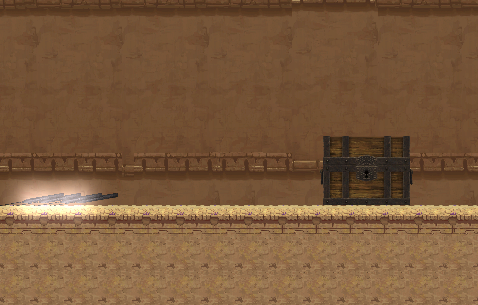
\includegraphics[width=6cm]{images/tyrek/skrzynia.png}
	\caption{Wytrychy i~skrzynia. Przykład z~projektu ,,The Lore''}
\end{figure}

Jeżeli gracz chce otworzyć skrzynie, nie posiadając w~ekwipunku żadnego wytrychu, otrzyma on informację o~tym fakcie poprzez komunikat na ekranie. Gdy użytkownik wybierze odpowiedni przycisk akcji, kamera zbliża się do skrzyni, po pewnym czasie rozpoczyna się mini-gra.

Na wstępie gracz jest informowany poprzez komunikat o~sterowaniu w~rozgrywce. Klawisze "\emph{Left}/\emph{RightButton}" są zależne od ustawień sterowania i~dotyczą przycisków poruszania się graczem w~lewo i~prawo. Jeżeli gracz wybierze któryś z~tych przycisków, wytrych przesunie się zgodnie z~jego poleceniem. Użytkownik jest informowany, czy jego ruch był poprawny.

\begin{figure}[h]
	\centering
	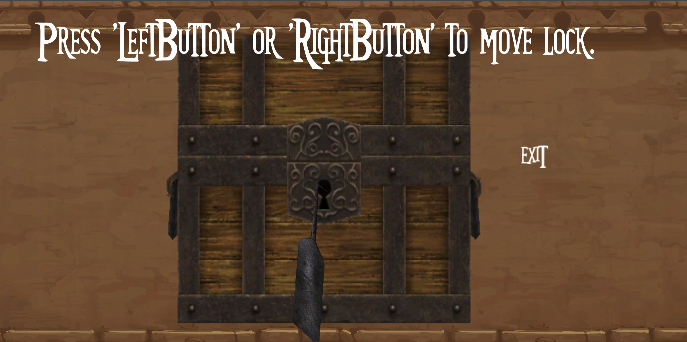
\includegraphics[width=6cm]{images/tyrek/minigraskrzynia.png}
	\caption{Mini-gra otwieranie skrzyń. Przykład z~projektu ,,The Lore''}
\end{figure}

Zadaniem gracza jest zgadnąć losowy ciąg elementów lewo/prawo o~długości 5. Każdy zły ruch powoduje konieczność powtórzenia sekwencji. Nagrodą za rozwiązanie problemu są eliksiry przywracające punkty życia, które przydają się w~czasie rozgrywki. Z~racji, iż jest to rozgrywka nieobowiązkowa, gracz w~każdej chwili może ją opuścić, wybierając opcję \textbf{Exit}.
\subsection{Przedstawienie przykładu w~innych grach}
\subsubsection{Mafia 2}
\par Gra Mafia II osadzona jest w~amerykańskim mieście rządzonym przez mafie. Głównym bohaterem jest Vito Scaletta, syn włoskich imigrantów. Los sprawia, iż bohater zmuszony jest do szybkiego zarobku, przez co wplata się w~mafijne porachunki. Realizując zadania dla swoich pracodawców, nieraz włamywał się do różnych pomieszczeń. 

\begin{figure}[h!]
	\centering
	\includegraphics[width=5cm]{images/tyrek/Mafia2.png}
	\caption{Otwieranie zamków. Przykład z~gry ,,Mafia 2''}
\end{figure}

Gracz może również w~czasie gry włamywać się do zamkniętych pokoi lub budynków, celem szybszego przejścia poziomu, obejścia wrogów czy zdobycia pieniędzy. Dodatkowo mini-gra pozwala na odblokowanie zamkniętych pojazdów. W~mini-grze gracz używa myszki. Widoczny jest zamek z~trzema zapadkami, po prawej stronie widzimy wytrych przy pierwszej zapadce. Użytkownik, sterując myszką wertykalnie, musi ustawić zapadkę w~takiej pozycji, aż będzie ona podświetlona na kolor zielony. Jeżeli gracz zrobi to w~złym momencie, zostanie cofnięty do poprzedniej zapadki. \cite{Mafia2}

\subsubsection{Assassin's Creed Unity}
\par W~grze ,,Assassin's Creed Unity'' wcielamy się w~Arno Doriana, członka tajnego bractwa Asasynów, którzy toczą odwieczną walkę z~organizacją zwaną Templariusze. Gra osadzona jest w~czasach rewolucji francuskiej w~Paryżu. Bohater, będąc w~centrum najważniejszych wydarzeń osiemnastowiecznego Paryża, nieraz potrzebuje włamać się do jakiegoś budynku, aby wykonać misję. W~grze otwieranie zamków dotyczy pomieszczeń, które dają podobnie jak w~poprzedniej grze, możliwość obejścia wrogów, czy też zdobycie ekwipunku oraz włamywania się do skrzyń – podobnie jak w~grze ,,The Lore''. Rozpoczynając mini-grę widzimy ilość zapadek, błękitny pasek poruszający się wertykalnie oraz błękitny prostokąt. 
\begin{figure}[h]
	\centering
	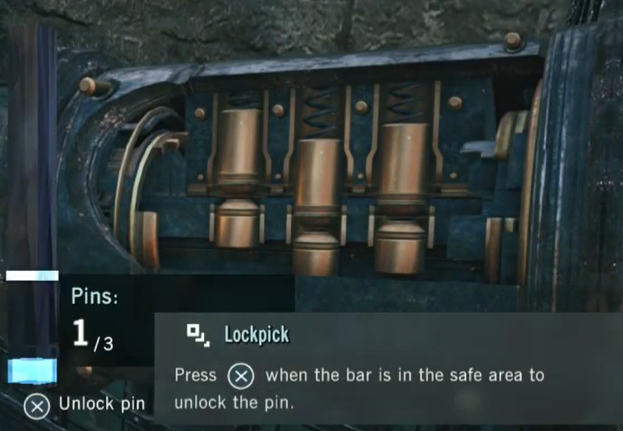
\includegraphics[width=6cm]{images/tyrek/acu.png}
	\caption{Otwieranie zamków. Przykład z~gry ,,Assassin Creed Unity''}s
	\end{figure}
Zadaniem gracza jest wcisnąć przycisk akcji w~momencie, gdy poruszający się znacznik znajdzie się w~błękitnym polu. W~przypadku, gdy gracz zrobi to w~złym momencie, traci z~ekwipunku wytrych. Warto też podkreślić, iż w~grze istnieje system umiejętności, gdzie dwie umiejętności dotyczą poziomu otwierania zamków. Podczas gry spotkamy trzy poziomy trudności, które charakteryzują się większą ilością zapadek czy też szybszym poruszaniem się błękitnego paska. \cite{acu}
\subsubsection{Gothic 2}
\par ,,Gothic 2'' to gra osadzona w~krainie Myrtana, w~której toczy się walka pomiędzy siłami dobra i~zła. Wcielamy się w~byłego więźnia kolonii więziennej, który w~wyniku pokonania Śniącego, tajemniczego potwora, niszczy magiczną barierę, która odcinała kolonię karną od reszty świata. Po upadku bariery bohater zostaje wybudzony przez nekromantę Xardasa, który informuje go o~nowych zagrożeniach, zagrażające krainie Myrtana. Gracz, sterując bohaterem, może dopuszczać się przestępstw, pozwalają mu one na zdobycie odpowiedniego ekwipunku czy złota. Może się to odbywać między innymi poprzez plądrowanie skrzyń w~chatach mieszkańców miasta Khorinis, czy też napotkanych, opuszczonych budynkach. 
Logika otwierania zamków, zarówno drzwi, jak i~skrzyń, jest dość podobna do zastosowanego systemu w~grze ,,The Lore''. Gracz, aby otworzyć daną skrzynie, musi posiadać wytrychy, które może zakupić od kupców w~mieście. Otwieranie skrzyń polega na odgadnięciu odpowiedniej sekwencji lewo – prawo, w~przypadku pomyłki gracz może utracić wytrych. Co ciekawe, gra nie losuje kolejności sekwencji. Jest ona stała dla danej skrzyni w~świecie gry, co może stanowić swego rodzaju ułatwienie – odpowiednie sekwencje można po prostu odnaleźć w~internecie.


\section{Labirynt}
\subsection{Omówienie zagadnienia}
\par W~pierwotnej definicji, labirynt oznacza budowlę, która charakteryzuje się układem dużej ilości pomieszczeń, które połączone są krętymi ciągami korytarzy. Oczywiście miało to na celu utrudnić dostęp do pewnego pomieszczenia osobom niepowołanym. Z~podobnych powodów w~niektórych grach mamy do czynienia z~labiryntem, zmuszając w~ten sposób gracza do szukania wskazówek, czy też zapamiętywaniu ścieżek, celem wyjścia z~labiryntu. 
\subsection{Algorytmika}
\subsubsection{Założenia: algorytm z~nawrotami}
Do stworzenia labiryntu można użyć algorytmu z~nawrotami. Początkowo należy stworzyć graf, gdzie każdy węzeł ma co najmniej jedno połączenie, to będzie labirynt. Pomiędzy węzłami, które nie są połączone, będzie znajdować się ściana, której użytkownik nie może przejść. Aby stworzyć taki graf, należy zacząć od generowania grafu bez ścieżek – można wyobrazić sobie, iż jest to po prostu prostokąt, podzielony na kilka kwadratów stworzonych przez ściany. Algorytm rozpoczyna się w~pierwszym węźle, dodając go do stosu. Następnie wybiera pierwszego nieodwiedzonego sąsiada, tworząc w~ten sposób pierwsze połączenie węzłów – z~punktu widzenia gracza, usuwając pomiędzy nimi ścianę. Proces powtarzany jest aż do momentu, gdy trafimy do węzła, które nie ma żadnego nieodwiedzonego sąsiada. Gdy algorytm już dotrze do takiego miejsca, cofa się, jednocześnie usuwając elementy ze stosu, aż do momentu trafienia na węzeł, który posiada nieodwiedzonego sąsiada. Algorytm skończy się, gdy w~naszym stosie nie będzie elementów. \cite{maze}

\subsubsection{Implementacja: algorytm z~nawrotami}
\par Na sam początek należy zdefiniować stany, które może posiadać każdy węzeł w~naszym grafie (labiryncie). Każdy węzeł może mieć ściany z~czterech stron.

\begin{lstlisting}[
language={[Sharp]C},
rulecolor=\color{blue!80!black},
caption={Stany danego węzła – skrypt C\#}
]
public enum NodeState
{
    LEFT = 1,
    RIGHT = 2,
    UP = 4,
    DOWN = 8,
    VISITED = 128
}
\end{lstlisting}
W~ten sposób można łatwo określić wszystkie ściany, które otaczają dany węzeł. Przykładowo, gdyby założyć, iż nasz węzeł otacza ściana lewa i~górna, stworzono by tu stan \textbf{NodeState nodeState = NodeState.LEFT | NodeState.UP}. Jak już wspomniano, celem jest, aby na początku wszystkie ściany tworzyły swego rodzaju siatkę, która odgradza każdy węzeł od innych. Generowanie jest w~tym przypadku bardzo proste, wystarczy w~odpowiedniej pętli wykonać odpowiednią liczbę iteracji \textbf{nodeWall[i] = NodeState.LEFT | NodeState.RIGHT | NodeState.UP | NodeState.DOWN}. Można również uznawać wartości za liczby binarne, \textbf{LEFT} jako 0001, \textbf{UP} 0010 i~tak dalej. Dany jest też stan odwiedzonego pola jako 128 – reprezentacja bitowa 1000 0000. W~przypadku, gdyby dodać do naszego obiektu nowy stan, wystarczy wykonać operację dodania alternatywy do obecnego stanu. \textbf{node[x,y] |= NodeState.VISITED} Oczywiście w~ramach większego porządku w~kodzie warto określić \textbf{nodeWall} jako tablicę dwuwymiarową, wyznaczając położenie w~osi poziomej i~pionowej. Pomoże to rozpoznać, w~jakim miejscu na labiryncie znajduje się dany węzeł. Jest to szczególnie przydatne, gdy tworzona będzie struktura pod pozycję każdego obiektu. Pozycje, tak jak wyżej wspomniano, przedstawiamy w~geometrii dwuosiowej, co oczywiście pomoże nam śledzić, gdzie znajduje się dany obiekt. 

\begin{lstlisting}[
language={[Sharp]C},
rulecolor=\color{blue!80!black},
caption={Pozycja obiektu – skrypt C\#}
]
public enum NodePosition
{
	public int x;
	public int y;
}
\end{lstlisting}
Warto też stworzyć strukturę do przechowywania informacji o~sąsiadach naszego węzła. Wystarczą wyżej przedstawione parametry \textbf{NodeState} i~\textbf{NodePosition}. Dodatkowo w~ramach kontroli należy stworzyć listę takich obiektów, które nie zostały jeszcze odwiedzone przez algorytm. Mając już takie struktury, kolejnym krokiem byłoby stworzenie metody, która zwraca nam stan danego sąsiada. Tak jak wspominano na początku, sąsiad będzie wybierany losowo, dlatego warto już na wstępie stworzyć obiekt \textbf{System.Random()}. Dzięki stworzonej wcześniej metodzie pobierania sąsiadów można go wybrać na przykład ze względu na kolejność na danej liście. Należy też stworzyć najważniejszy dla algorytmu z~nawrotami stos. Każdy odwiedzony węzeł powinien być oznaczony wartością \textbf{NodeState.VISITED} i~dodany do tego stosu. Wystarczy, aby były to obiekty \textbf{NodePosition}, jednak nic nie zaszkodzi, aby były to całe obiekty \textbf{NodeState}. Teraz dzięki pętli while, należy sprawdzać kolejne węzły, dopóki stos nie będzie pusty. Jeżeli ostatnio dodany do stosu obiekt posiada co najmniej jednego sąsiada, to należy pobrać ich listę, przy użyciu funkcji losującej i~wybrać dany element z~posiadanej listy. Następnie trzeba dodać do stosu wylosowany obiekt oraz usunąć każdą odwiedzoną ścianę.

Następnie powinniśmy usunąć każdą odwiedzoną ścianę.

\begin{lstlisting}[
language={[Sharp]C},
rulecolor=\color{blue!80!black},
caption={Usunięcie ściany – skrypt C\#}
]
node[x, y] &= ~neighbour.SharedWall;
\end{lstlisting}

Gdzie \textbf{SharedWall} mówi o~tym, czy pomiędzy dwoma obiektami znajduje się ściana. Oczywiście, informacja o~ścianie powinna zostać zaktualizowana również u~sąsiada. W~tej sytuacji są dwa wyjścia. Pierwszy z~nich, z~lekka naiwny i~niezbyt przyjazne dla oka dewelopera to stworzenie czterech warunków, które definiują dla danego przypadku jak pobrać pozycję przeciwną, dla sąsiada po lewej stronie – prawo, dla sąsiada na dole – góra i~tak dalej. W~ten sposób możemy zdobyć węzeł i~zmienić jego stan, a~następnie dodać nowy element do stosu. Drugim, rozsądniejszym pomysłem jest zadeklarowanie metody, która mogłaby od razu zwrócić nam \textbf{NodeState} naszego sąsiada, który od razu mógłby być szybko poprawiony. Z~pomocą przychodzi tutaj prosta instrukcja switch(), która pozwala nam na zarządzanie czterema przypadkami, z~którymi będziemy mieli do czynienia.


\begin{lstlisting}[
language={[Sharp]C},
rulecolor=\color{blue!80!black},
caption={Zwracanie stanu sąsiada – skrypt C\#}
]
switch(nodeState)
{
	case NodeState.RIGHT =  return  NodeState.LEFT;
	case NodeState.LEFT = return  NodeState.RIGHT;
	case NodeState.UP =  return NodeState.DOWN;
	case NodeState.DOWN = return NodeState.UP;
}
\end{lstlisting}

Algorytm gotowy. W~tym momencie mamy stworzony generator labiryntu, następnym krokiem powinno być wizualne stworzenie obiektu. Dzięki otrzymanym informacjom nie sprawia to większych problemów. Mając informację o~wszystkich węzłach, można stworzyć pętle, która tworzy obiekty ścian ze względu na ściany istniejące dla danego węzła. Z~pomocą przychodzi tu obiekt \textbf{Instantiate}. Służy on do klonowania przekazanego obiektu (w~tym przypadku ściany labiryntu). Dodatkowo metoda ta pozwala na określenie dokładnej pozycji oraz rotacji naszego elementu, co pozwoli na ułożenie ściany w~wyznaczonym miejscu i~pozwoli na obrócenie obiektu – ze względu czy jest ścianą pionową, czy poziomą. Dokładny obiekt, który jest potrzebny to \textbf{Instantiate(Object original, Vector3 position, Quaternion rotation)}. \cite{Instantiate}

Teraz używając czterech warunków, dla każdej strony, można zweryfikować, czy nasz węzeł sąsiaduje z~daną ścianą. Dla każdej ściany (jeśli istnieje) tworzymy jej obiekt. Następnie należy określić pozycję – tutaj przychodzi z~pomocą obiekt \textbf{Vector3}. Jest to trójelementowa struktura, która przydaje się w~określaniu między innymi pozycji w~trzech osiach – \textbf{Vector3(x, y, z)}. \cite{Vector3}. Pozycja jest tutaj zależna od wymagań dewelopera – należy dopasować ją do wielkości naszego obiektu. Z~pomocą przychodzi Unity, które w~sekcji \textbf{Inspector} pozwala łatwo zarządzać wielkością danego obiektu. Rotacja potrzebuje zaś już czteroelementowego obiektu – \textbf{Quaternion}. Ze względu na posiadany obiekt ściany, deweloper musi określić, która oś powinna zostać zmieniona. W~ten sposób powinien wygenerować się widoczny labirynt.

\subsection{Przedstawienie przykładu w~innych grach}
\subsubsection{Wriggler}
\par ,,Wriggler'' jest grą wydaną w~1985 roku. W~grze sterujemy robakiem, którego zadaniem jest uciec z~labiryntu składającego się z~256 poziomów, w~ramach wyścigu, w~którym bierze udział. Każdy poziom (labirynt) jest stały – nie są one generowane w~czasie gry.  \cite{Wriggler}


\begin{figure}[h!]
	\centering
	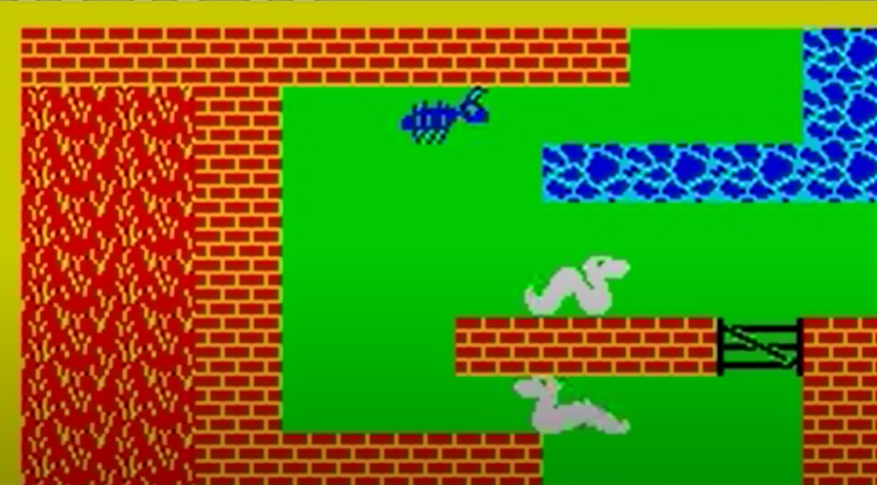
\includegraphics[width=7cm]{images/tyrek/wriggler.png}
	\caption{Labirynt. Przykład z~gry Wriggler}
\end{figure}

\subsubsection{Dandy}
\par Kolejną grą opartą na labiryntach jest \textbf{Dandy}. Gra powstała w~1983 roku na platformy Atari, przez Johna Howarda Palevicha, w~ramach pracy licencjackiej na MIT. Gracz steruje postacią, poruszając się po lochach z~wieloma poziomami, które połączone są ze sobą schodami. Niektóre fragmenty labiryntu zamknięte są przez drzwi, do których otwarcia potrzebne są klucze, rozsiane po planszy. Oprócz pokonywania kolejnych poziomów gracz może pokonywać wrogów przy użyciu łuku. \cite{Dandy}
\clearpage
\section{Podsumowanie}
\par Jak widać, projektowanie zagadek logicznych jako mini-gry może nie być aż tak trudne. Dużo zależy od podejścia autora i~kreatywności w~przewidywaniu szczególnych sytuacji – czego przykładem jest kwestia nierozwiązywalnych przesuwanych puzzli. Pomocne jest tu też narzędzie Unity i~zawarte w~nim funkcjonalności. Dzięki odpowiednim dopasowaniom komponentów do obiektów można łatwo testować produkt pod kątem potencjalnych błędów. Na pewno wielkim plusem jest tu też szeroka dokumentacja Unity, która pozwala twórcom łatwo znaleźć funkcje, czy obiekty, które mogą się przydać w~toku tworzenia własnej rozgrywki.

\chapter{Fizyka postaci}
\section{Tworzenie postaci}
\subsection{Omówienie zagadnienia procesu tworzenia postaci}
Zagadnienie procesu tworzenia postaci polega na przygotowaniu grafik tak, żeby można było swobodnie wprowadzić i~pracować na projekcie postaci w~Unity. Proces ten obejmuje również stworzenie odpowiednich komponentów przygotowanych bezpośrednio w~celu animowania odpowiednich kończyn, jak i~późniejszej pracy na kolizjach. Przedstawione są więc aspekty przygotowania graficznego postaci, jak i~późniejszego wprowadzenia jej do projektu w~taki sposób, żeby można było tworzyć na niej odpowiednie kolizje, animacje i~skrypty odpowiadające za poruszanie się.
\subsection{Proces graficzny tworzenia postaci}
Tworzenie postaci zaczyna się od projektu graficznego, który jest kluczowym punktem do późniejszego animowania postaci. Należy wziąć pod uwagę wszystkie ograniczenia i~korzyścii, jakie daje nam stworzenie projektu w~odpowiedni sposób. Istnieją 2 najbardziej popularne sposoby tworzenia graficznego postaci, które pozwalają na animowanie jej.

Pierwsza możliwość to statyczny bohater, będący bazą do tworzenia animacji poklatkowych, które później używane są bezpośrednio w~projekcie. Główną zaletą takiego rozwiązania są bardzo dobrze wyglądające animacje, wynikające z~braku ograniczeń ilości zmian w~postaci w~trakcie animowania.
Proces ten wymaga jednak dużego nakładu czasu poświęconego na modelowanie postaci w~konkretnych pozach, symulowanie konkretnych ruchów oraz tworzenie zmian w~postaci takich jak np. poruszające się włosy przy skoku.

Alternatywą dla tego rozwiązania jest użycie kinematyki odwrotnej, która bazuje na systemie kości w~ciele postaci, połączeń i~ograniczeń ich ruchów. Rozwiązanie to jest dużo bardziej wydajne czasowo, nie wymaga dużych umiejętności w~animowaniu i~pozwala na wprowadzanie nowych animacji wynikających z~rozwoju projektu wewnątrz środowiska Unity. Animacja stworzona z~użyciem kinematyki odwrotnej jest wykonywana w~czasie rzeczywistym, przez co nie ma potrzeby tworzenia odpowiedniej ilości klatek, żeby wyglądała płynnie (ma tyle samo klatek co gra w~konkretnym momencie wykonywania animacji).
W praktyce przekłada się to na konieczność tworzenia grafiki w~odpowiedni sposób. Należy podzielić postać na osobne warstwy odpowiadające za ilość kończyn, które powinny się ruszać w~końcowym projekcie.\\

\begin{figure}[h]
	\centering
	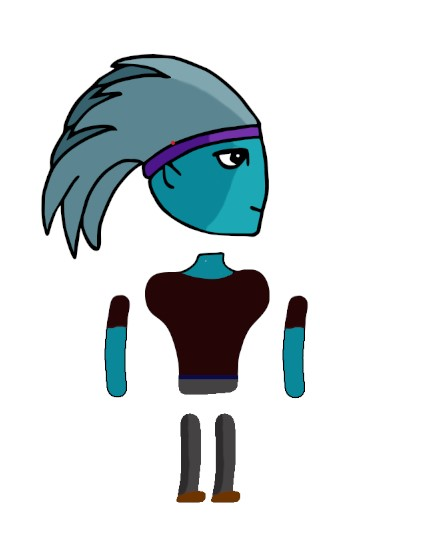
\includegraphics[width=6cm]{images/kozubal/separatedCharacter.jpg}
	\caption{Projekt graficzny postaci w~edytorze Gimp}
\end{figure}

Postać w~rozważanym projekcie jest podzielona odpowiednio na głowę, tors, ręce i~nogi. Liczba możliwych komponentów nie jest ograniczona. Tak przygotowany projekt graficzny w~formacie PSB jest gotowy do importu w~środowisku Unity, a~poszczególne warstwy są widoczne jako oddzielne komponenty. Tym samym projekt jest gotowy do dalszej pracy.

\subsection{Wdrożenie postaci do projektu w~Unity}
W celu zaimportowania postaci w~Unity z~projektu graficznego niezbędna jest biblioteka o~nazwie \textbf{\textit{PSDImporter}}, która pozwala na bezproblemowe wdrożenie projektu w~tym formacie jako gotowy do pracy \textbf{\textit{sprite}} \footnote{\textbf{\textit{Sprite}} – Dwuwymiarowy obrazek używany w~systemach grafiki komputerowej}. W~kolejnym etapie należy nadać postaci kości odpowiadające konkretnym kończynom oraz geometrię postaci.

\begin{figure}[h]
	\centering
	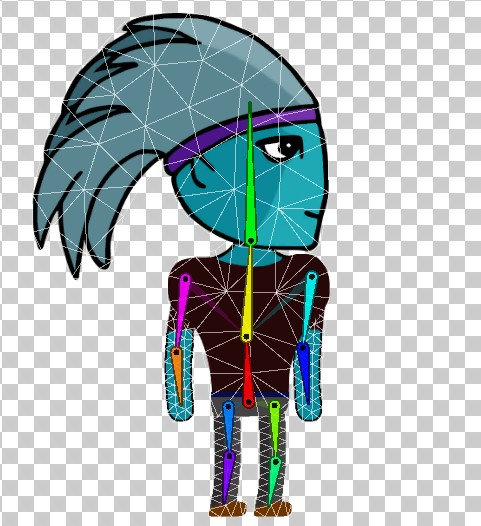
\includegraphics[width=6cm]{images/kozubal/bones.jpg}
	\caption{Widok postaci w~środowisku Unity – kości}
\end{figure}

Geometria postaci to siatka, która definiuje, w~jaki sposób postać może się zgiąć w~trakcie animowania, a~kości powodują ograniczenie ruchów w~taki sposób, aby były one naturalne, jednocześnie łącząc ze sobą wcześniej powstałe warstwy. W~celu uniknięcia przesuwania się torsu w~trakcie poruszania rękami lub nogami należy wykluczyć zależność tych kości między sobą. W~praktyce podczas ruchu ręką nie jest zaangażowany cały kręgosłup.
Następnym i~ostatnim krokiem wdrożeniowym jest zapisanie zmian i~przeniesienie wygenerowanej postaci do sceny oraz dodanie do każdej kończyny kinematyki odwrotnej. Tak spreparowana postać jest gotowa do pracy w~animatorze Unity.



\subsection{Sposoby animowania postaci}
Głównym celem animacji jest stworzenie iluzji. Najlepiej postrzegane animacje to te, które w~realistyczny sposób odwzorowują żywą postać.

 \newpage
Głównym zadaniem animatora jest przestrzeganie zasad animacji w~taki sposób, aby finalnie ruch postaci był jak najbardziej zbliżony do naturalnego ruchu człowieka.
Zadanie to niejednokrotnie jest utrudnione, ponieważ dotyczy wykreowanego świata i~narysowanych w~programie postaci, jednak zważając na wcześniej przygotowany system kości, jesteśmy w~stanie przynajmniej podobnie odwzorować sam ruch postaci. 
Proces animowania rozpoczynamy od stworzenia animatora, czyli obiektu odpowiedzialnego za obsługę i~włączanie konkretnych animacji w~danym momencie niejednokrotnie po spełnieniu warunków przejścia do konkretnej animacji. \cite{animation1} \\
W naszym projekcie taki animator prezentuje się następująco:

\begin{figure}[h]
	\centering
	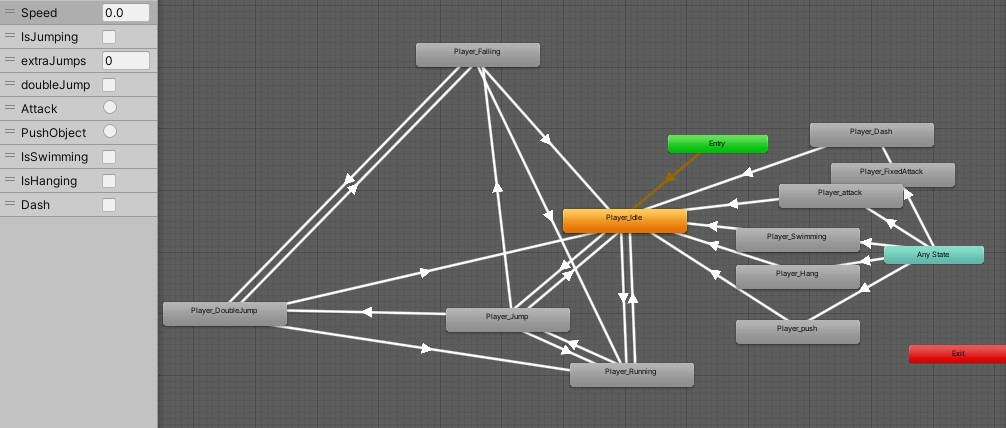
\includegraphics[width=13cm]{images/kozubal/animator.jpg}
	\caption{Widok animatora projektu ,,The Lore''}
\end{figure}

Po lewej stronie widoczne są warunki, które podpięte są do konkretnych stanów przejścia między animacjami, np. wartość zmiennej \textbf{\textit{IsJumping}} służy do określenia, kiedy możemy przejść do animacji skoku. Animacje dodajemy do animatora poprzez stworzenie nowego pliku animacji, cały proces przebiega już na tym pliku. W~oknie pojawia się oś czasu na której możemy zdefiniować kolejne etapy animacji.\\

\begin{figure}[h]
	\centering
	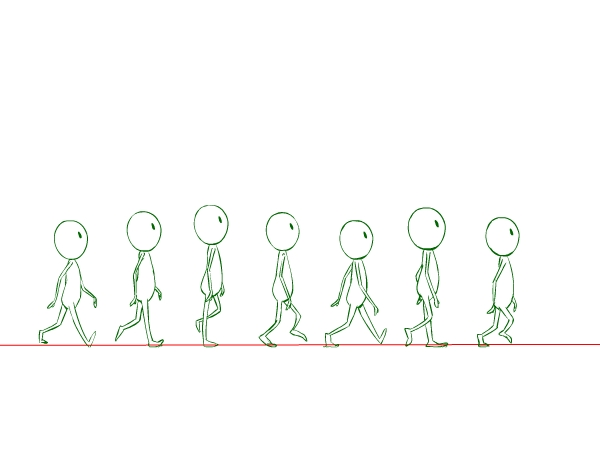
\includegraphics[width=10cm]{images/kozubal/walkingAnimation.jpg}
	\caption{Animacja chodzenia – przykład ze strony design.tutsplus.com \cite{animation2}}
\end{figure}

\newpage W~tym momencie korzystamy ze wcześniejszego przygotowania postaci. Animacja poklatkowa polega na przedstawieniu ruchu klatka po klatce, w~praktyce dzięki animatorowi możemy stworzyć przejścia tylko między bardziej istotnymi etapami animacji. Osobno animowany jest ruch ciała, głowy, kończyn, a~całość zamiast kilkuset zdjęć sprowadza się do kilku stanów, które automatycznie przechodzą między sobą w~naturalny sposób.

\begin{figure}[h]
	\centering
	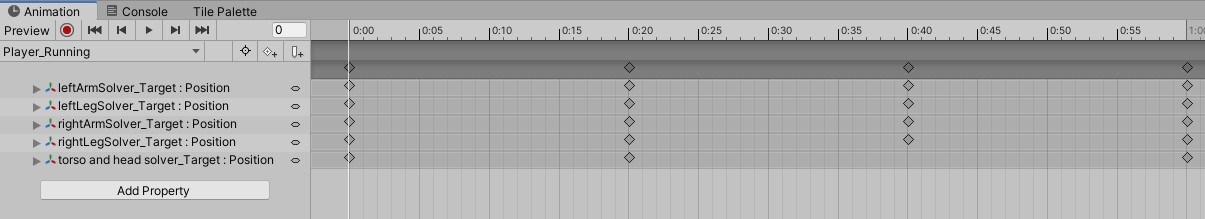
\includegraphics[width=13cm]{images/kozubal/runningAnimation.jpg}
	\caption{Animacja biegania – widok z~projektu ,,The Lore''}
\end{figure}

Animacja biegu w~projekcie posiada tylko 4 stany, z~których ostatni jest taki sam jak pierwszy w~celu zapętlenia animacji. W~praktyce więc animowanie w~Unity to próba przedstawienia w~jak najbardziej rzeczywisty sposób czynności życia codziennego w~taki sposób, aby stworzyć iluzję realizmu. Jeśli jednak czynność nie występuje w~realnym świecie jak np. umiejętności, animacja jest stworzona w~taki sposób, aby wyglądać jak najbardziej naturalnie w~swojej abstrakcji.

\section{Poruszanie się}
\subsection{Omówienie zagadnienia}
Zagadnienie poruszania się dotyczy całego procesu skryptowego postaci. Elementy potrzebne do przygotowania postaci do środowiska deweloperskiego, jak i~wszelkie aspekty wprowadzenia postaci w~ruch oraz jej reakcje na wejście wprowadzane przez użytkownika. W~tej części pracy przedstawione zostaną problemy związane z~tworzeniem poszczególnych funkcjonalności oraz sposoby ich rozwiązania. Zostanie również przedstawiony szczegółowy proces implementacji poszczególnych funkcjonalności, jak i~sposoby ich wdrożenia. W~tym rozdziale również zostanie przedstawiona fizyka postaci oraz poszczególne elementy, które pokrywają się z~fizyką świata rzeczywistego, a~które od takiej fizyki odbiegają.
\subsection{Fizyka w~grach 2D, a~w~prawdziwym świecie}
Na pojęcie fizyki w~grach składają się dwa główne komponenty, jednym z~nich jest silnik fizyki, natomiast drugim silnik kolizji. Pomimo że silnik fizyki jest zależny od silnika kolizji, nie zajmują się one tym samym.
Silnik kolizji dzieli się na dwie części: detekcja kolizji oraz jej responsywność, która jest częścią silnika fizyki, z~tego faktu oba te silniki przeważnie występują w~jednej bibliotece. Wykrywanie kolizji występuje w~dwóch formach: ciągłej i~oddzielnej. Używanie ciągłej detekcji jest bardzo kosztowne w~zasoby oraz może skutkować dużymi spadkami wydajnościowymi, dlatego w~grach używa się jej tylko wtedy, kiedy naprawdę jest potrzebna. W~większości wypadków sprowadza się to do tego, że zamiast zatrzymywać użytkownika przed wbiegnięciem w~ścianę, jego pozycja jest zmieniana już, kiedy w~tę ścianę częściowo wbiegnie, podobnie jest z~podłożem. W~prawdziwym świecie naturalnie nie istnieje możliwość wbiegnięcia w~ścianę i~ponownej teleportacji we wcześniejsze miejsce i~nie jesteśmy ograniczeni sposobami wydajnościowymi. Jeśli chodzi o~wykrywanie kolizji z~wykorzystaniem ruchomych obiektów, początków łamigłówek, kolizji z~podłożem w~celu możliwości skoku czy kontaktu z~przeciwnikiem, używamy do tego pustego obiektu usytuowanego w~postaci w~celu sprawdzania kolizji od tego obiektu. Często wysunięty jest on w~konkretnym kierunku, w~którym w~danym momencie musimy sprawdzać konkretne kolizje. Sprawdzanie kolizji sprowadza się do stworzenia otoczenia wokół naszego obiektu w~postaci człowieka (wielkość takiego koła często zależy od konkretnej sytuacji, do której chcemy go użyć), a~następnie sprawdzenie, czy kolizja tego obiektu nie nachodzi na żaden inny obiekt z~otoczenia. \cite{physics1}


\begin{lstlisting}[breaklines=true,
language={[Sharp]C},
rulecolor=\color{blue!80!black},
caption={Fragment klasy \texttt{CharacterController.cs}}
]
for (int i~= 0; i < colliders.Length; i++)
{
   if (colliders[i]
                  .gameObject
                  .name
                  .Contains("Moving Platform")) {
      onMovingPlatform = true;
      currentPlatform = 
      = colliders[i].gameObject.GetComponent<MovingPlatform>();
   }

   if (colliders[i].gameObject != gameObject)
   {
      m_Grounded = true;
   }

   if (!wasGrounded)
   {
   animator.SetBool("IsJumping", false);
   }

}
\end{lstlisting}

W skrypcie jest sprawdzana konkretna warstwa lub konkretny obiekt, z~którym oczekujemy konkretnego działania po kolizji.
Ta część kodu odpowiada za sprawdzenie, czy postać dotyka ziemi w~celu ustawienia zmiennej na odpowiadającą jej wartość, a~także za sprawdzenie, czy postać jest na poruszających się platformach w~celu późniejszej zmiany jej rodzica.
W tym momencie, kiedy kontakt został odkryty, jesteśmy w~stanie stwierdzić dokładnie, kiedy występuje kolizja między dwoma konkretnymi obiektami i~pracować na nich lub ograniczać je zależnie od tego.

\subsection{Poruszanie się oraz kolizje postaci}
Za poruszanie się w~projekcie ,,The Lore'' odpowiedzialne są dwie klasy: CharacterController.cs i~PlayerMovement.cs. Ta pierwsza odpowiedzialna jest za sam ruch, skok i~wyświetlanie postaci w~dobrym kierunku, natomiast druga zajmuje się resztą animacji od przesuwania przedmiotów po używanie umiejętności. Ze względu na to, że w~projekcie użyty jest model bryły sztywnej Unity, otwiera on wiele ścieżek pracy nad postacią. Aby wprowadzić postać, w~ruch musimy znać kierunek, w~którym chcemy, żeby się poruszyła oraz docelową prędkość.


\begin{lstlisting}[breaklines=true,
language={[Sharp]C},
rulecolor=\color{blue!80!black},
caption={Fragment klasy \texttt{CharacterController.cs}}
]
Vector3 targetVelocity =
= new Vector2(move * 10f, m_Rigidbody2D.velocity.y);

m_Rigidbody2D.velocity = Vector3.SmoothDamp(
              m_Rigidbody2D.velocity, 
              targetVelocity, 
              ref m_Velocity, 
              m_MovementSmoothing);
\end{lstlisting}

Zmienna \textbf{\textit{targetVelocity}} odpowiedzialna jest za określenie konkretnego ruchu, który chcemy, żeby wykonała postać. Warto zauważyć, że końcowy wynik jest wygładzany przy pomocy wbudowanej do wektora metody \textbf{\textit{SmoothDamp}} \cite{physics2}, co oznacza, że ruch nie jest sztywny i~ma swoje ograniczenia czasowe w~trakcie jego wykonywania. W~praktyce przenosi się to na bardziej intuicyjny sposób poruszania się, jak i~poprawę wizualną samego ruchu.
Kolejną wcześniej wspomnianą funkcjonalnością, którą zajmuje się ta klasa, jest zmienianie kierunku grafiki w~zależności od kierunku, w~którym się poruszamy.


\begin{lstlisting}[breaklines=true,
language={[Sharp]C},
rulecolor=\color{blue!80!black},
caption={Fragment klasy \texttt{CharacterController.cs}}
]
private void Flip()
{
   m_FacingRight = !m_FacingRight;
   Vector3 theScale = transform.localScale;
   theScale.x *= -1;
   transform.localScale = theScale;
}
if (move > 0  &&  !m_FacingRight  &&  !Statics.isOnRope)
{
   Flip();
}
else if (move < 0  &&  m_FacingRight  &&  !Statics.isOnRope)
{ 
   Flip();
}
\end{lstlisting}

Metoda \textbf{\textit{Flip()}} odpowiedzialna jest za zmianę skali lokalnej postaci poprzez pomnożenie jej wartości przez -1 i~wykonywana jest po sprawdzeniu wstępnych założeń.

Kolejnym sposobem implementacji ruchu jest odejście od używania wbudowanego modelu bryły sztywnej oraz wartości prędkości do niej przypisanej i~zamiast tego używanie przejścia poprzez aktualizację wartości pozycji postaci. Problemy, jakie generuje to rozwiązanie to konieczność przeliczania praw tarcia i~ruchu oraz przypisywania ich w~kodzie i~analogicznej zmiany pozycji pokrywającej te prawa. Przez rozbudowany system fizyki w~Unity takie rozwiązanie nie ma większego sensu i~powoduje konieczność włożenia dodatkowej pracy. Niemniej jednak istnieją sytuacje, w~których takie rozwiązanie sprawdza się lepiej niż np. symulacja bujania się na linach czy nawet sam skok.
Jednymi z~głównych kolizji odpowiedzialnych za sam etap poruszania się są kolizje z~podłożem oraz ze ścianami (ze względu na wymiar gry kolizja z~sufitem nie jest brana pod uwagę). Podobnie jak wspomniano wcześniej, kolizje te definiują, kiedy możemy przejść dalej oraz kiedy postać ma możliwość skoku, która odnawia się za każdym razem, kiedy postać ponownie dotknie podłoża. Warto pamiętać, żeby oddzielić warstwy podłoża od warstw innych obiektów posiadających kolizje, gdyż może to przynieść niechciane efekty w~postaci zwiększonej ilości skoków w~obszarze obiektu posiadającego kolizję.

\subsection{Skakanie} 
Skok jest kluczowym elementem w~grach, niezależnie od tego, czy mowa o~grach platformowych, czy MMO-RPG, skakanie jest nie tylko jedynym lub jednym z~głównych sposobów dostania się na wyższe poziomy, ale również główną mechaniką dotyczącą przemieszczania się. Niektórzy użytkownicy preferują ciągły skok jako alternatywę dla biegania tylko dlatego, że wydaje się ona szybsza. Większość gier obala jednak tezę, że skok jest szybszy niż bieg, ale są też takie gry, które specjalnie implementują taką mechanikę, jednym z~takich przykładów jest Counter Strike: Global Offensive, gdzie poprzez umiejętne wykorzystanie skoku można poruszać się kilkukrotnie szybciej, niż biegnąc. Skakanie jest preferowaną metodą poruszania się też ze względu na większą ilość możliwości ruchu w~trakcie skoku.
Czym tak naprawdę jest skok w~grach 2D i~jak dużo wspólnego ma z~rzeczywistą fizyką? Bardzo dużo gier symuluje skok jak najbardziej zbliżony do rzeczywistej fizyki, istnieją jednak gry, które implementują inne rozwiązanie. Dobrym przykładem jest znana gra platformowa Mario, ale również takie gry jak Limbo, Cuphead, speedrunners gdzie podczas skoku stawia się na inne rozwiązanie. \cite{jumping1} 

\begin{figure}[h]
	\centering
	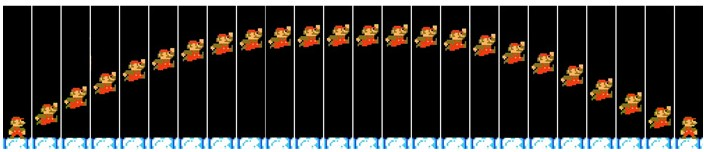
\includegraphics[width=13cm]{images/kozubal/mario.jpg}
	\caption{Przykład skoku z~gry Super Mario Maker 2 \cite{jumping3}}
\end{figure}

\newpage
Jak można zauważyć na obrazku, skok nie jest parabolą, tak jak byłoby w~przypadku realistycznej sytuacji. W~niektórych grach 2D tworzy się symulację skoku polegającą na tym, że im dłużej trzyma się przycisk skoku, tym dłużej jest się w~powietrzu. W~rzeczywistości polega to na ustawieniu czasu, w~którym siła może działać na postać i~ograniczenia jej górnego limitu. W~praktyce kiedy tylko przestaniemy trzymać przycisk skoku, postać automatycznie zacznie lecieć w~dół, a~jeśli go przytrzymamy, zawiśnie ona na chwilę w~powietrzu. Stało się to na tyle powszechne, że taka symulacja skoku wydaje się bardziej naturalna niż dodanie do niego wertykalnej siły jednorazowo, czyli zgodnie z~prawami fizyki. \cite{jumping2} \\ W~naszym projekcie zdecydowaliśmy się na rzeczywistą symulację fizyki. Stworzenie skoku w~taki sposób pozwala na większą przewidywalność miejsca lądowania, kosztem mniejszej kontroli samego skoku. Implementacja skoku w~projekcie The Lore prezentuje się następująco:

\begin{lstlisting}[breaklines=true,
language={[Sharp]C},
rulecolor=\color{blue!80!black},
caption={Fragment klasy \texttt{CharacterController.cs}}
]
if(m_Grounded && jump){
   m_Grounded = false;
   m_Rigidbody2D.AddForce(new Vector2(0f, m_JumpForce));
   jump = false;
   onMovingPlatform = false;
}
if(!m_Grounded && jump && extraJumps > 0 && !Statics.isOnRope){
   m_Rigidbody2D.velocity =
   = new Vector2(m_Rigidbody2D.velocity.x, 0);
   animator.SetBool("doubleJump", true);
   m_Rigidbody2D.AddForce(new Vector2
                         (0f,m_JumpForce * extraJumpDifficulty)
                         );
   jump = false;
   extraJumps--;
}
\end{lstlisting}
\newpage
Obsługa skoku w~naszym projekcie polega zatem na jednorazowym dodaniu siły do postaci w~trakcie skoku. Rozważana sytuacja jest bardziej skomplikowana, jeśli chodzi o~wielokrotny skok, ze względu na jednokrotne dodanie siły. Przed ponownym skokiem aktualna prędkość wertykalna musi zostać ustawiona na 0 ze względu na to, że skok dodaje wartość siły do aktualnej wartości działającej na postać. W~trakcie wielokrotnego skoku bez ustawienia tej wartości na 0 przyczyniłoby się to do spowolnienia, a~nie wykonania kolejnego skoku.

\subsection{Otoczenie wpływające na fizykę postaci}
W grach niejednokrotnie pojawiają się obiekty oddziałujące na fizykę naszej postaci. Ich symulacja często wiąże się z~niewymiernym odwzorowaniem rzeczywistej fizyki. W~tym podrozdziale głównym opisywanym narzędziem, z~którego korzystamy, będzie wcześniej wspomniane wykrywanie kolizji między konkretnymi obiektami. Jeśli chcemy, żeby obiekt lub nasza postać zachowywała się w~konkretny sposób, po kontakcie ze sobą trzeba ten kontakt i~konkretny obiekt najpierw wykryć. Dobre nazewnictwo warstw i~obiektów przydaje się nie tylko do symulowania samej fizyki, ale również do łatwego nawigowania po animacjach, a~nawet włączania samej animacji z~poziomu skryptu, a~nie animatora. Na samym początku warto spojrzeć na skrypt służący do przesuwania skrzyń.


\begin{lstlisting}[breaklines=true,
language={[Sharp]C},
rulecolor=\color{blue!80!black},
caption={Fragment klasy \texttt{PlayerMovement.cs}}
]
void MoveObject(){
   if (Physics2D.OverlapCircleAll(actionPoint.position, 
                                  boxMoveRange, 
                                  boxLayer
                                  ).Length > 0 
   && !animator.GetBool("IsJumping")){
      Physics2D.OverlapCircleAll(actionPoint.position,
                                  boxMoveRange,
                                  boxLayer)[0]
                                 .GetComponent<BoxMoving>()
                                 .MoveBox(direction);
      animator.SetTrigger("PushObject");
   }
}
\end{lstlisting}

Jest to bardzo prosty skrypt, w~którym jedyne siły dochodzące do dotychczas oddziałujących to waga skrzyń, które chcemy przesunąć. To ciężar skrzyń sprawia, że postać po zbliżeniu się do skrzyni i~próbie jej przesunięcia znacznie spowalnia i~skutkuje to ruchem skrzyni, której fizyka jest symulowana poprzez model bryły sztywnej dodany bezpośrednio do skrzyni.
W naszym projekcie są jeszcze 2 obiekty oddziałujące na fizykę postaci, pierwszym z~nich są ruchome platformy. Symulacja stania na platformie jest uproszczona ze względu na grywalność i~jest ona niczym innym jak dodaniem platformy jako rodzica naszej postaci, co skutkuje tym, że platforma nie porusza się w~kontekście postaci (ruch na platformie jest taki sam jak na ziemi). Mimo to dodana została siła poruszającej się platformy przy samym wyskoku. Jeśli obiekt, na którym znajduje się postać, jest w~ruchu, to po wyskoku do góry postać nasza powinna poruszać się w~tym samym kierunku i~z taką samą prędkością co platforma w~trakcie wyskoku. Dlatego skok w~którąkolwiek stronę będzie wypadkową siły skoku oraz prędkości poruszającej się aktualnie platformy.

\begin{lstlisting}[breaklines=true,
language={[Sharp]C},
rulecolor=\color{blue!80!black},
caption={Fragment klasy \texttt{PlayerMovement.cs}}
]
if (onMovingPlatform && !m_Grounded)
{
   move += currentPlatform.velocityX;
   onMovingPlatform = false;
}
\end{lstlisting}
Przez to, że aktualna prędkość przyjmuje wartości ujemne, gdy porusza się w~lewą stronę, a~dodatnie, gdy porusza się w~prawą, implementacja tego problemu ogranicza się do kilku linijek.
Kolejnym obiektem oddziałującym na fizykę postaci w~grze ,,The Lore'' są liny. Mechanika lin polega na tym, że jeśli postać znajduje się wystarczająco blisko odpowiedniego obiektu oraz przytrzyma przycisk chwytu to przestanie spadać i~zawiśnie na linie. Ponadto w~takiej sytuacji postać może poruszać całą liną i~bujać się w~celu przeskoczenia dalej. Problem ten jest dużo bardziej złożony, samo symulowanie lin w~Unity działa bardzo dobrze, aczkolwiek dużo bardziej powszechnym rozwiązaniem jest ręczna symulacja i~stworzenie do tego problemu animacji poklatkowej lub ewentualna zmiana pozycji postaci w~taki sposób, aby uniknąć konkretnego usytuowania gracza względem liny i~tym samym niepożądanego efektu. Problem ten w~projekcie ,,The Lore'' został rozwiązany poprzez przesunięcie obiektu szukającego kolizji z~linami na przód gracza i~zmniejszenia go w~taki sposób, aby pole, w~którym może się złapać gracz było małe. Likwiduje to potencjalne problemy z~niechcianym chwytem. Rozwiązanie takie sprawia, że mechanika jest poniekąd trudniejsza do ukończenia. Po testach użytkowników okazało się jednak, że wciąż nie jest ona wystarczająco trudna, dlatego usunięty został jeden z~możliwych dodatkowych skoków po zeskoczeniu z~liny.

\newpage
\begin{lstlisting}[breaklines=true,
language={[Sharp]C},
rulecolor=\color{blue!80!black},
caption={Fragment klasy \texttt{PlayerMovement.cs}}
]    
Collider2D[] colliders = Physics2D.OverlapCircleAll
(actionPoint.position, attackRange, ropeLayer);
if (colliders.Length > 0 && !Statics.isOnRope)
{
   recentCollider = colliders[0];
   FixedJoint2D joint = colliders[0]
                        .gameObject
                        .AddComponent<FixedJoint2D>();
   joint.connectedBody = gameObject.GetComponent<Rigidbody2D>();
   isOnRope = true;
   Statics.isOnRope = true;
   controller.extraJumps = 1;
}

\end{lstlisting}

Problem trzymania się liny został rozwiązany przy użyciu połączenia stałego między postacią a~jednym z~obiektów lin, ponieważ lina sama w~sobie składa się z~kilkunastu fragmentów połączonych. Aby uniknąć błędów przy połączeniu, brana jest pod uwagę tylko jedna z~wykrytych przez skrypt kolizji. Warto zaznaczyć też, że bujanie liną jest możliwe ze względu na możliwość ruchu postaci w~powietrzu. Gdyby nie to rozwiązanie trzeba by było zmodyfikować klasę dotyczącą poruszania się tak, aby ruch był możliwy również w~trakcie kontaktu z~liną. Połączenie stałe między postacią a~liną zostaje zerwane w~momencie puszczenia przycisku akcji, po czym użytkownikowi przysługuje jeszcze jeden skok.

\section{Umiejętności postaci}
\subsection{Omówienie zagadnienia umiejętności}
Umiejętności postaci to nowe mechaniki wprowadzone do gry w~celu zarówno zwiększenia dynamiki rozgrywki, jak i~ulepszenia doznań użytkownika. Sekcja ta poświęcona będzie zarówno projektowi, jak i~mechanikom wewnątrz całego drzewka umiejętności, a~także całemu procesowi projektowemu i~problemom związanym z~poszczególnymi umiejętnościami. Przedstawione zostanie przygotowanie graficzne drzewka, jak i~różne sposoby na implementację tych samych umiejętności.

\subsection{Drzewko umiejętności}
Drzewko umiejętności to dodatkowa mechanika w~grze, pozwalająca użytkownikowi na rozwijanie poszczególnych gałęzi według własnych upodobań. To w~tym miejscu gracz jest w~stanie samemu określić, w~jaki sposób projektować będzie rozwój postaci oraz w~jaki sposób przebiegać będzie jego rozgrywka. W~celu zwiększenia dynamiki rozgrywki można postawić głównie na umiejętności związane z~poruszaniem się, jeśli jednak użytkownik jest bardziej zapobiegawczym typem gracza, bardziej prawdopodobnie skupi się na przetrwaniu i~sile.
\subsubsection{Wstępny prototyp drzewka, a~widok końcowy}
Drzewko umiejętności w~projekcie ,,The Lore'' w~fazie prototypowania prezentowało się następująco:


\begin{figure}[h]
	\centering
	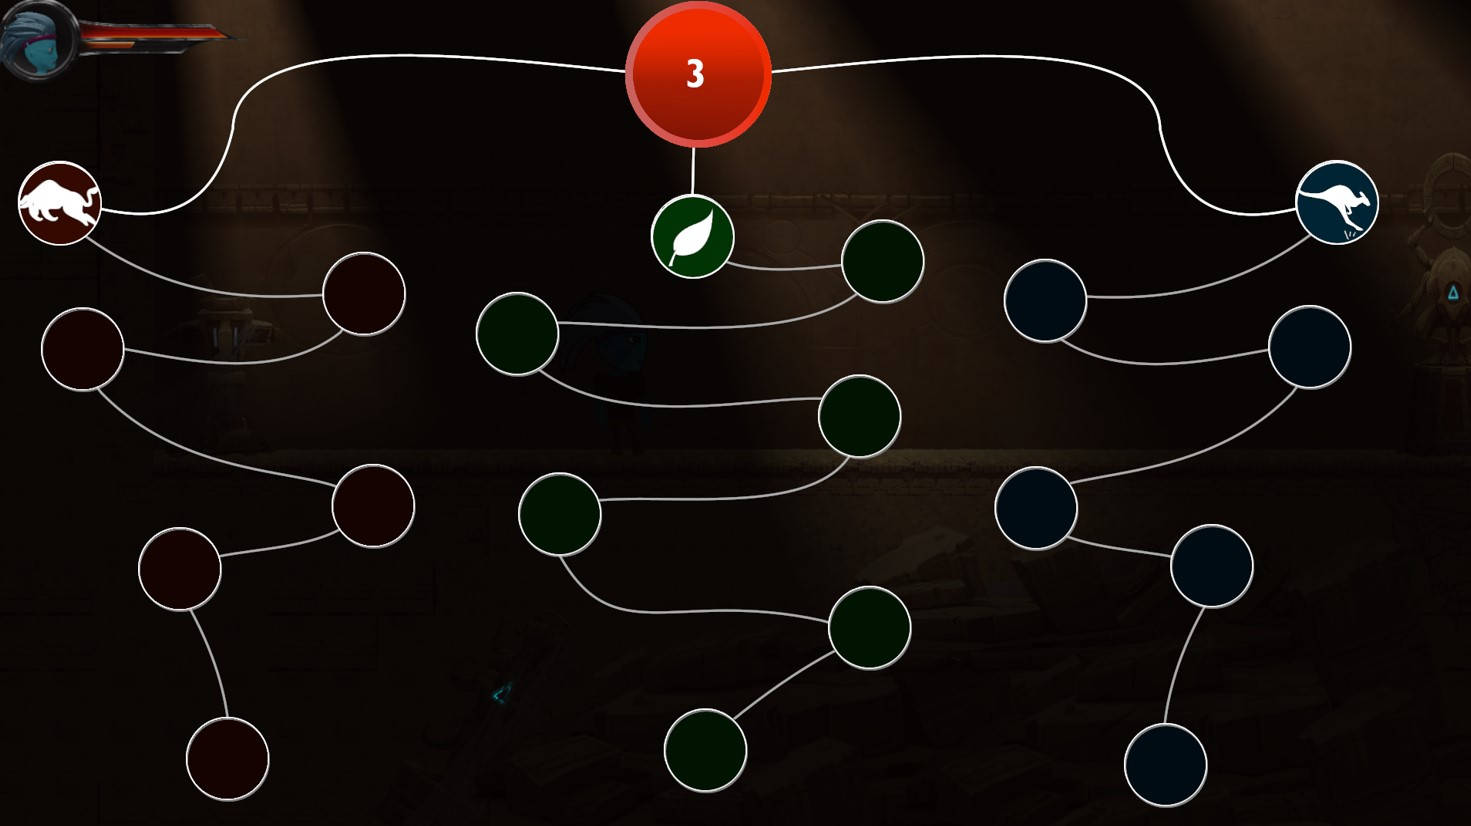
\includegraphics[width=13cm]{images/kozubal/drzewkoPrototyp.jpg}
	\caption{Prototyp drzewka w~projekcie ,,The Lore''}
\end{figure}

Jak okazało się w~kolejnych fazach pracy i~testach użytkowników taka ilość umiejętności jest nieproporcjonalna do ilości treści i~możliwości zdobytych poziomów w~grze, dlatego w~końcowej iteracji drzewo zostało ograniczone do 3 umiejętności na jedną gałąź. Widok końcowy bazujący na prototypie wygląda następująco:


\begin{figure}[h]
	\centering
	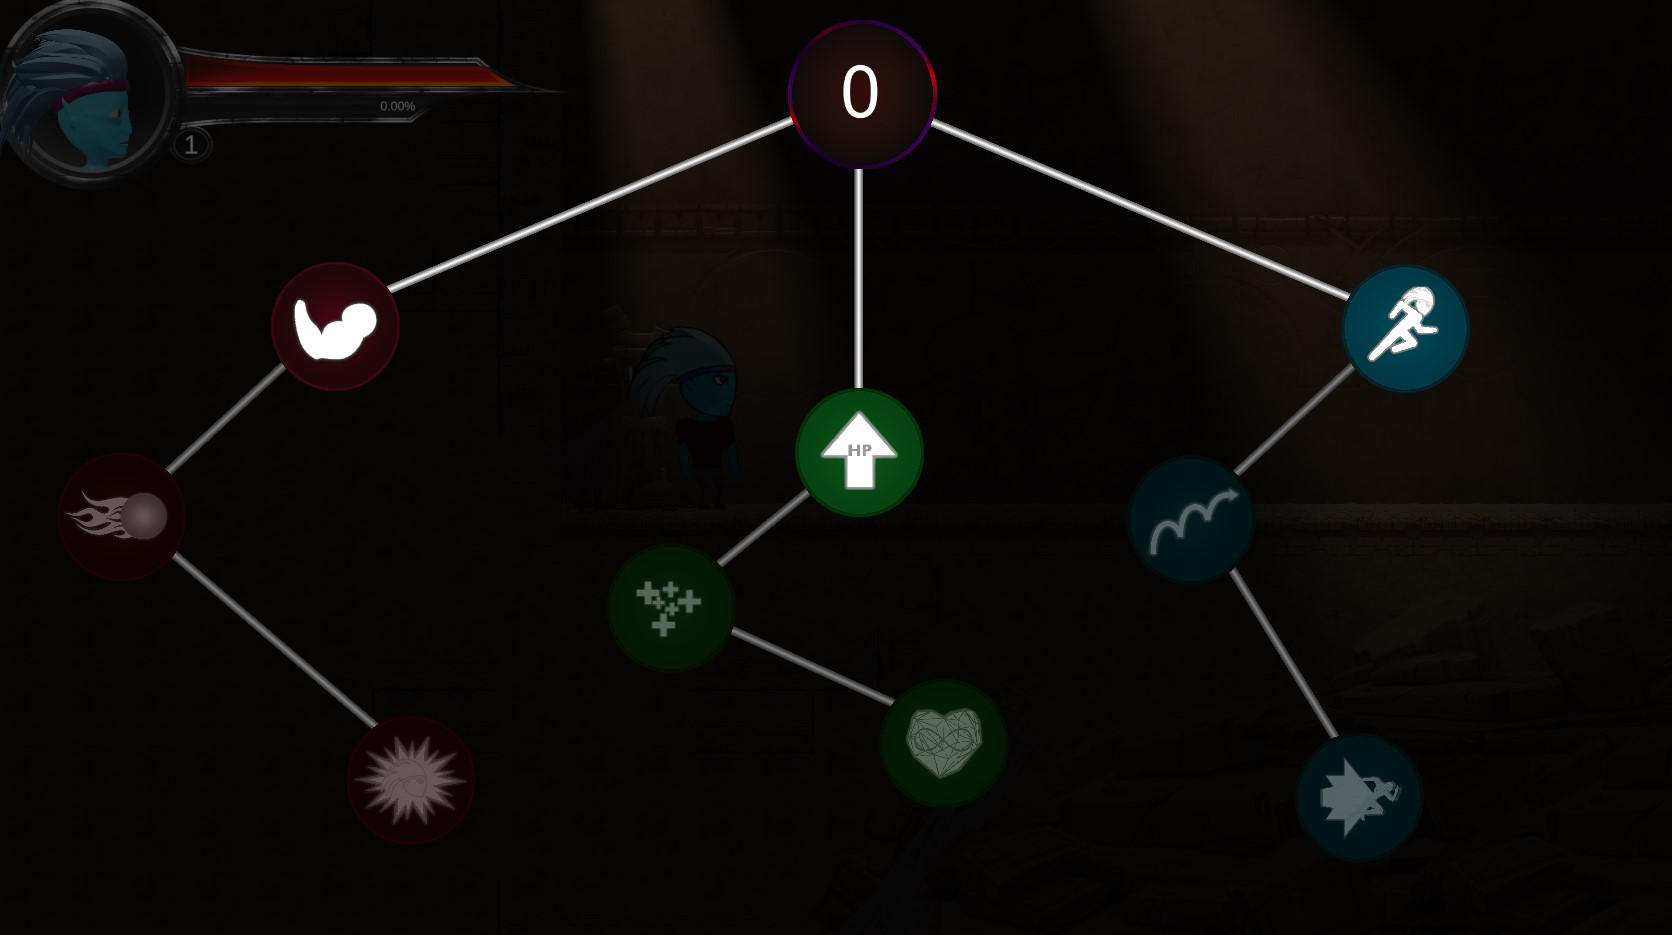
\includegraphics[width=13cm]{images/kozubal/drzewkoTheLore.jpg}
	\caption{Aktualne drzewko umiejętności w~projekcie ,,The Lore''}
\end{figure}
\newpage
Górny licznik wyświetla, ile umiejętności jesteśmy w~stanie w~danym momencie rozwinąć, tzn. ile dostępnych punktów umiejętności jest aktualnie odblokowanych. Liczba ta jest przeliczana w~następujący sposób:


\begin{lstlisting}[breaklines=true,
language={[Sharp]C},
rulecolor=\color{blue!80!black},
caption={Fragment klasy \texttt{UI\_SkillTree.cs}}
]    
text = (GLOBAL_DATA.Instance.Level - 1 - unlockedSkills)
\end{lstlisting}

W praktyce w~sytuacji braku odblokowanych umiejętności wskaźnik wyświetla zawsze o~jeden punkt mniej niż aktualny poziom postaci. Przez to wystarczy odjąć od tego jeszcze długość listy obiektów typu \textbf{SkillButton} i~końcowy wynik pokazuje aktualną ilość punktów. Podobne sprawdzenie używane jest w~klasie \textbf{PlayerSkills.cs}, w~celu weryfikacji czy użytkownik może daną umiejętność rozwinąć. Kolejnym ważnym punktem, przy sprawdzaniu poszczególnych umiejętności, jest ich hierarchia, czyli odblokowywanie umiejętności z~danej gałęzi w~odpowiedniej kolejności. Tym zadaniem zajmuje się następujący fragment kodu:

\newpage
\begin{lstlisting}[breaklines=true,
language={[Sharp]C},
rulecolor=\color{blue!80!black},
caption={Fragment klasy \texttt{PlayerSkills.cs}}
]    
public SkillType GetSkillRequirement(SkillType skillType) {
   switch (skillType) {
      //Blue Skills Requirements
      case SkillType.TripleJump: return SkillType.Sprint;
      case SkillType.Dash: return SkillType.TripleJump;
      //Red Skills Requirements
      case SkillType.Bullet: return SkillType.IncreaseDMG;
      case SkillType.Explode: return SkillType.Bullet;
      //Green Skills Requirements
      case SkillType.RegenerationHP: return SkillType.ExtraHP;
      case SkillType.Immortality: return SkillType.RegenerationHP;
   }
return SkillType.None;
}
\end{lstlisting}

Zwracana wcześniejsza umiejętność przy próbie odblokowania pozwala nam określić, która umiejętność jest warunkiem do odblokowania danej umiejętności, co znacznie ułatwia sprawdzanie, wystarczy przeszukać listę odblokowanych umiejętności i~sprawdzić, czy wcześniejsza w~hierarchii istnieje w~danym kontekście.

\subsubsection{Przykłady z~innych gier}
Jest wiele gier, które wykorzystują drzewka umiejętności po to, żeby ułatwić użytkownikowi rozgrywkę. Istnieją jednak takie gry, których podejście do drzewek umiejętności jest inne, są implementowane po to, żeby gracz poradził sobie na wyższych poziomach trudności lub nawet są mechaniką, bez której samej gry nie jesteśmy w~stanie przejść. Dobrym przykładem takiej gry jest Path of Exile, w~której liczba ścieżek w~drzewku, które możemy wybrać, jest ogromna, a~samo drzewko prezentuje się następująco:

\begin{figure}[h]
	\centering
	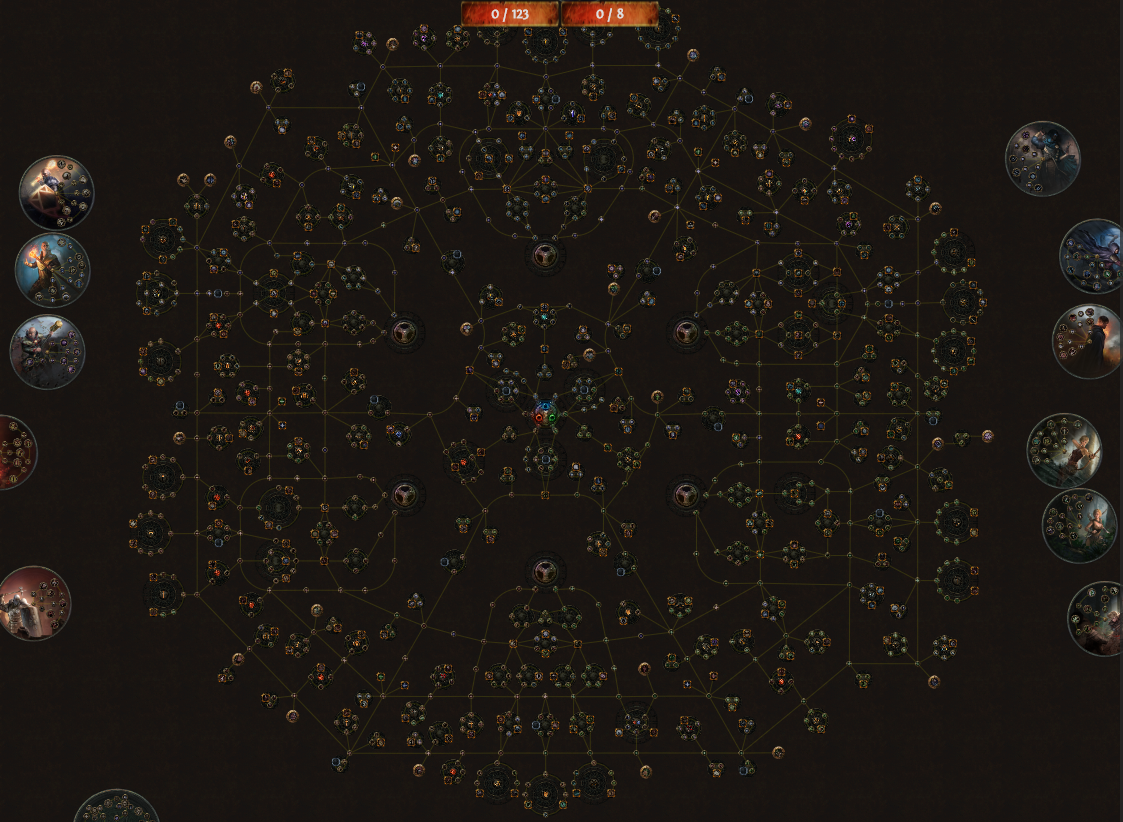
\includegraphics[width=11cm]{images/kozubal/poe.png}
	\caption{Drzewko Umiejętności z~gry Path of Exile }
\end{figure}
\newpage
W omawianym projekcie zastosowano prostszy model drzewka ze względu na ograniczoną liczbę poziomów oraz możliwości ich zdobycia. Przykładem użycia podobnego drzewka umiejętności jest gra Ori And The Blind Forest, w~której drzewko to wygląda następująco:

\begin{figure}[h]
	\centering
	\includegraphics[width=9cm]{images/kozubal/ori.jpg}
	\caption{Drzewko Umiejętności z~gry Ori And The Blind Forest}
\end{figure}
\subsection{Umiejętności}
W tej sekcji skupimy się głównie na umiejętnościach zaimplementowanych w~projekcie, problemach(jeśli owe istniały) i~innym sposobie rozwiązania tych samych problemów w~trakcie tworzenia umiejętności.

\subsubsection{Umiejętności siły}
Zwiększenie mocy – odpowiedzialne za zwiększenie siły ataku podstawowego do 130-250\% przez 2 sekundy. Wartość z~tego przedziału jest losowana z~każdym użyciem umiejętności.
Eksplozja – Postać ładuje obszar dookoła siebie o~określonym promieniu i~zadaje obrażenia każdemu wrogowi znajdującemu się w~tym obszarze, dodany do tego został system cząstek dla lepszej wizualizacji efektu.
Strzał z~kuli – Postać wystrzeliwuje horyzontalnie kulkę lecącą ze stałą prędkością w~kierunku, w~którym aktualnie patrzy się postać, umiejętność ta jest zrobiona ciągłym aktualizowaniem pozycji kulki o~daną, stałą wartość i~zadawanie obrażeń każdemu przeciwnikowi, którego napotka na swojej ścieżce. Kolejnym sposobem rozwiązania tego problemu jest stworzenie kuli jako bryły sztywnej oraz symulowanie trajektorii lotu kuli. Na potrzeby projektu oraz w~danym kontekście oczekiwanym rezultatem był jednak lot po prostej, poziomej drodze, dlatego zdecydowaliśmy się na pierwsze rozwiązanie.

\begin{figure}[h]
	\centering
	\includegraphics[width=9cm]{images/kozubal/sila.png}
	\caption{Ikony umiejętności siły z~projektu ,,The Lore''}
\end{figure}
\subsubsection{Umiejętności poruszania się}
Umiejętności poruszania się służą głównie do łatwiejszego/płynniejszego przemieszczania się po planszy, jak i~większej opcjonalności przy unikaniu ataków przeciwników, 3 umiejętności dotyczące poruszania się w~naszym projekcie to:
Sprint – Polega na zwiększeniu prędkości gracza w~trakcie trzymania klawisza, mechanikę tę możemy kojarzyć między innymi z~takich gier jak Super Mario Bros.
Potrójny skok – Polega na możliwości wykonania dodatkowego skoku w~trakcie lotu, domyślna wartość to dwa. Umiejętność ta pozwala na doskoczenie we wcześniej niedostępne miejsca, a~także na większą swobodę w~locie.
Pęd – Trzecia i~ostatnia umiejętność z~gałęzi poruszania się polega na bardzo szybkim przemieszczeniu się horyzontalnym gracza. Jest to często wykorzystywana mechanika w~grach platformowych takich jak np. Ori And The Blind Forest. Istnieje kilka sposobów rozwiązania tego problemu. Najłatwiejszym z~nich jest zmiana pozycji postaciprzy pierwszej okoliczności, generuje to jednak problemy związane z~ewentualnymi przeszkodami, jak i~z płynnością takiego przejścia. Kolejnym rozwiązaniem, które zostało użyte w~naszym projekcie, jest przez określoną ilość czasu aktualizowanie konkretnej pozycji gracza, ponownie pojawia się tu problem wchodzenia w~ściany, natomiast jest on w~tym wypadku dużo łatwiejszy do rozwiązania. Przez to, że pozycja nie jest zmieniana jednokrotnie, tylko stopniowo, przez pewien odstęp czasu jesteśmy w~stanie sprawdzać, czy istnieje przed postacią jakaś przeszkoda w~trakcie wykonywania się skryptu i~opcjonalnie przestać wykonywać umiejętność w~trakcie, gdy przeszkoda znajduje się przed postacią.


\begin{lstlisting}[breaklines=true,
language={[Sharp]C},
rulecolor=\color{blue!80!black},
caption={Fragment klasy \texttt{PlayerSkills.cs}}
]    
if (dashValue < dashForce && dash && !touchingWall)
{
   Dash();
}
\end{lstlisting}
\begin{figure}[h]
	\centering
	\includegraphics[width=9cm]{images/kozubal/movement.png}
	\caption{Ikony umiejętności poruszania się z~projektu ,,The Lore''}
\end{figure}
\subsubsection{Umiejętności przetrwania}
Umiejętności przetrwania przydają się wtedy, kiedy bardzo dużo giniemy od przeciwników. Pozwalają one na dużo większą beztroskę w~trakcie walki z~przeciwnikami, jak i~na uzupełnianie swojego życia poza nią. W~naszym projekcie wyróżniamy takie umiejętności jak:
Zwiększenie życia – Jest to umiejętność pasywna zwiększająca na stałe poziom zdrowia gracza ze 100 do 125, co przyczynia się do tego, że jesteśmy w~stanie przetrwać więcej ciosów od przeciwników, tym samym gra bardziej wybacza nasze błędy.
Odnowienie życia – Jest to umiejętność aktywna, w~trakcie naciśnięcia przycisku do użycia umiejętności jesteśmy w~stanie raz na 30 sekund odnowić swoje życie o~25, przyczynia się to do spowolnienia rozgrywki, jednocześnie dając możliwość odnowienia sobie życia przed lub w~trakcie walki z~mocniejszymi przeciwnikami.
Nieśmiertelność – Jest to umiejętność aktywna pozwalająca nam przez 2 sekundy być odpornymi na każdy atak przeciwnika. Zastosowań tej umiejętności jest mnóstwo. Może ona posłużyć nam do ucieczki przed przeciwnikiem w~kryzysowej sytuacji, jak i~pomóc nam w~zadaniu mu dodatkowych ciosów nie tracąc przy tym punktów zdrowia. 


\begin{figure}[h]
	\centering
	\includegraphics[width=9cm]{images/kozubal/patience.png}
	\caption{Ikony umiejętności przetrwania z~projektu ,,The Lore''}
\end{figure}

\section{Podsumowanie}
Podsumowując, w~rozdziale tym został przedstawiony proces tworzenia postaci, przeniesienia jej do środowiska pracy oraz samą pracę na niej, jeśli chodzi o~poruszanie się i~główne aspekty z~tym związane. Warto pamiętać, że nie wszystkie gry odwzorowują fizykę w~taki sposób, jak wygląda ona rzeczywiście, dlatego dobrze jest znać zagrania, którymi kierują się deweloperzy przy projektowaniu odpowiednich mechanik, a~w grach 2D istnieje dużo ukrytych sposobów rozwiązywania problemów i~innego przedstawienia fizyki, do którego większość użytkowników jest przyzwyczajona, przez co dokładna symulacja fizyki dla przeciętnego gracza wydaje się mniej poprawna niż użycie tych sztuczek.

\begin{thebibliography}{100} 

\addtolength{\leftmargin}{0.2in} 
\setlength{\itemindent}{-0.2in}

\bibitem {unity}
Wikipedia, Wolna Encyklopedia. Unity (silnik gry), dostęp w~internecie 15.12.2020r.\\
\url{https://pl.wikipedia.org/wiki/Unity\_(silnik\_gry)}

\bibitem{projekt}
Robert K. Wysocki, Rudd McGary: \emph{Efektywne zarządzanie projektami.} Wydanie III, ISBN: 83-7361-861-9, dostęp w~internecie 25.01.2021r.\\
\url{http://pdf.onepress.pl/efzapr/efzapr-1.pdf}

\bibitem{projekt2}
CorazLepszyPortalBiznesowy. \emph{Co to jest projekt?}, dostęp w~internecie 25.01.2021r.\\
\url{https://www.corazlepszyportalbiznesowy.pl/art/co-to-jest-projekt}

\bibitem{projekt3}
NaRUDO. \emph{Co to jest projekt i~dlaczego się nim zarządza?}, dostęp w~internecie 25.01.2021r.\\
\url{https://narudo.pl/co-to-jest-projekt/}

\bibitem{zarzadzanie8}
The balance careers. \emph{Basic Project Management 101}, dostęp w~internecie 26.01.2021r.\\
\url{https://www.thebalancecareers.com/project-management-101-2275338}

\bibitem{zarzadzanie7}
Frączkowski K.: \emph{Zarządzanie projektem informatycznym}\\
Oficyna Wydawnicza Politechniki Wrocławskiej, Wrocław 2003.\\
ISBN 83-7085-731-0, dostęp w~internecie 27.01.2021r\\
\url{https://www.dbc.wroc.pl/Content/998/fraczkowski\_zarzadzanie\_projektem.pdf}

\bibitem{IO- Helion}
Bernd Bruegge, Allen H. Dutoit: \emph{Inżynieria oprogramowania w~ujęciu obiektowym. UML, wzorce projektowe i~Java}.\\
Helion, ISBN: 978 - 83-24 6 -2872-8, dostęp 27.01.2021r.

\bibitem{zarzadzanie5}
Indeed. \emph{5 Phases of the Project Management Life Cycle}, dostęp w~internecie 28.01.2021r.\\
\url{https://www.indeed.com/career-advice/career-development/phases-of-project-management-life-cycle\#3C}

\bibitem{testJ}
Devpark. \emph{Testowanie aplikacji – testy integracyjne, jednostkowe i~smoke test}, dostęp w~internecie 28.01.2021r.\\
\url{https://devpark.pl/pl/testowanie-aplikacji-testy-integracyjne-jednostkowe-i-smoke-testy/}

\bibitem {testI}
Wikipedia, Wolna Encyklopedia. \emph{Testy integracyjne}, dostęp w~internecie 28.01.2021r.\\
\url{https://pl.wikipedia.org/wiki/Testy\_integracyjne}

\bibitem {testO}
Kaliop. \emph{Testy obciążeniowe}, dostęp w~internecie 28.01.2021r.\\
\url{https://www.kaliop.pl/Blog/Artykuly/Testy-obciazeniowe-czyli-jak-weryfikujemy-stabilne-dzialanie-aplikacji-internetowych}

\bibitem {testF}
TESTERKA. \emph{Testy funkcjonalne}, dostęp w~internecie 29.01.2021r.\\
\url{http://testerka.pl/testy-funkcjonalne/}

\bibitem {testA}
ForProgress. \emph{Testy Akceptracyjne}, dostęp w~internecie 29.01.2021r.\\
\url{https://forprogress.com.pl/testy-akceptacyjne/}

\bibitem{modele}
NaRUDO. \emph{Zwinne i~tradycyjne zarządzanie projektami}. dostęp w~internecie 30.01.2021r.\\
\url{https://narudo.pl/zwinne-i-tradycyjne-zarzadzanie-projektam/}

\bibitem{agileVwaterfall}
global4net. \emph{Waterfall czy Agile – którą metodykę wybrać?}, dostęp w~internecie 30.01.2021r.\\
 \url{https://global4net.com/ecommerce/waterfall-czy-agile-ktora-metodyke-wybrac/}

\bibitem{waterfall}
Wikipedia, Wolna Encyklopedia. \emph{Model kaskadowy}, dostęp w~internecie 30.01.2021r.\\
\url{https://pl.wikipedia.org/wiki/Model\_kaskadowy}

\bibitem{agile}
Agile247. \emph{Czym jest agile?}, dostęp w~internecie 31.01.2021r.\\
\url{https://agile247.pl/agile/}

\bibitem{agile2}
Harvard Business Review. \emph{Embracing Agile}, dostęp w~internecie 31.01.2021r.\\
\url{https://hbr.org/2016/05/embracing-agile}

\bibitem{wykresy}
ScienceSoft. \emph{8 Software Development Models: Sliced, Diced and Organized in Charts}.  dostęp w~internecie 30.01.2021r.\\
\url{https://www.scnsoft.com/blog/software-development-models}

\bibitem{Agile game}
Marionette. \emph{Agile Game Development – a~Quick Overview}. dostęp w~internecie 01.02.2021r.\\
\url{https://marionettestudio.com/agile-game-development-quick-overview/}

\bibitem{agilePract}
starloop. \emph{Best Agile Practices in Game Development}, dostęp w~internecie 01.02.2021r.\\
\url{https://starloopstudios.com/best-agile-practices-in-game-development/}

\bibitem{agileHunt}
Agile Hunters. \emph{Role w~Scrum}, dostęp w~internecie 02.02.2021r.\\
\url{https://agilehunters.com/role-w-scrum/}

\bibitem{kanban}
LUQAM. \emph{Kanban – czym jest, cele i~efekty}, dostęp w~internecie 02.02.2021r.\\
\url{https://www.luqam.com/kanban-czym-jest-cele-i-zastosowanie/}

\bibitem{jira}
Żurkowski M: \emph{Jira: wszystko, co potrzebujesz wiedzieć}, dostęp w~internecie 02.02.2021r.\\
\url{https://blog.deviniti.com/pl/atlassian-pl/jira-wszystko-co-potrzebujesz-wiedziec/}

\bibitem{VPC}
PRODUCTVISION, \emph{Value Proposition Canvas – unikalna propozycja wartości modelu biznesowego}, dostęp w~internecie 03.02.2021r.\\
\url{https://productvision.pl/2014/value-proposition-canvas-unikalna-propozycja-wartosci-modelu-biznesowego/}

\bibitem{BMC}
PRODUCTVISION, \emph{Business Model Canvas – szablon modelu biznesowego}, dostęp w~internecie 03.02.2021r.\\
\url{https://productvision.pl/2014/business-model-canvas-szablon-modelu-biznesowego/}

\bibitem{zagadka_logiczna} 
Wikipedia, Wolna Encyklopedia.”, \emph{Zagadka} dostęp 07.01.2021r.
\\ \url{https://pl.wikipedia.org/wiki/Zagadka}

\bibitem{rebus} 
Wikipedia, Wolna Encyklopedia.”, \emph{Rebus}, dostęp 07.01.2021r.
\\ \url{https://pl.wikipedia.org/wiki/Rebus}

\bibitem{przesuwane_puzzle}
Wikipedia, Wolna Encyklopedia.”, \emph{15 puzzle}, dostęp 07.01.2021r.
\\ \url{https://en.wikipedia.org/wiki/15\_puzzle}

\bibitem{puzzle}
Wikipedia, Wolna Encyklopedia.”, \emph{Puzzle}, dostęp 07.01.2021r.
\\ \url{https://pl.wikipedia.org/wiki/Puzzle}

\bibitem{scena}
Unity Documentation, \emph{Creating Scenes}, dostęp 09.01.2021r.
\\ \url{https://docs.unity3d.com/Manual/CreatingScenes.html}

\bibitem{gameobject}
Unity Documentation, \emph{GameObject} dostęp 09.01.2021r.
\\ \url{https://docs.unity3d.com/ScriptReference/GameObject.html}

\bibitem{komponent}
Unity Documentation, \emph{Component} dostęp 28.01.2021r.
\\ \url{https://docs.unity3d.com/ScriptReference/Component.html}

\bibitem{solvablePuzzle}
Geeks for geeks. Check instance 8 puzzle solvable, dostęp 26.01.2021r.
\\ \url{https://www.geeksforgeeks.org/check-instance-8-puzzle-solvable/}

\bibitem{pipemania}
Wikipedia, Wolna Encyklopedia.” \emph{Pipe Mania}, dostęp 27.01.2021r.
\\ \url{https://en.wikipedia.org/wiki/Pipe\_Mania}

\bibitem{Mafia2}
Mafia Wiki, Fandom, \emph{Lock Picking}, dostęp 28.01.2021r.
\\ \url{https://mafiagame.fandom.com/wiki/Lock\_Picking}

\bibitem{acu}
IGN, Assassin's Creed Unity Wiki Guide, \emph{Lockpick}, dostęp 28.01.2021r.
\\ \url{https://www.ign.com/wikis/assassins-creed-5-unity/Lockpick}

\bibitem{maze}
Qaz Wiki: \emph{Algorytm generowania labiryntu - Maze generation algorithm}, dostęp 02.02.2021r.
\\ \url{https://pl.qaz.wiki/wiki/Maze\_generation\_algorithm}

\bibitem{nd}
Fandom Wiki, \emph{The Haunting of Castle Malloy}, dostęp 03.02.2021r.
\\ \url{https://nancydrew.fandom.com/wiki/The\_Haunting\_of\_Castle\_Malloy}

\bibitem{Instantiate}
Unity Documentation, \emph{Instantiate}, dostęp 04.02.2021r.
\\ \url{https://docs.unity3d.com/ScriptReference/Object.Instantiate.html}

\bibitem{Vector3}
Unity Documentation, \emph{Vector3}, dostęp 04.02.2021r.
\\ \url{https://docs.unity3d.com/ScriptReference/Vector3.html}

\bibitem{Wriggler}
Personal Computer News, \emph{Issue 107}, dostęp 04.02.2021r.
\\ \url{http://www.personalcomputernews.co.uk/pcnb/html/107/personal\_computer\_news\_107\_gameplay\_spectrum\_the\_wriggler.html}

\bibitem{Dandy}
 "a~History of Dandy Dungeon", Jack Palevich. Wersja archiwizowana z~04.11.2013r. Dostęp 04.02.2021 r.
\\ \url{https://web.archive.org/web/20131104190048/http://jacks-hacks.appspot.com/dandy/history.html}

\bibitem{sp}
"Soda Pipes", Mobby Games. Dostęp 04.02.2021r.
\\ \url{https://www.mobygames.com/game/windows/soda-pipes}
\bibitem{animation1}
"Animation of 2d character in Unity", gamedevacademy. Dostęp 29.01.2021r.
\\ \url{https://gamedevacademy.org/how-to-animate-a-2d-character-in-unity/}
\bibitem{animation2}
"Animation for beginners", tutsplus. Dostęp 01.02.2021r.
\\ \url{https://design.tutsplus.com/tutorials/animation-for-beginners-how-to-animate-a-character-running--cms-25730}
\bibitem{physics1}
"How does a~collision engine work", Stack Exchange. Dostęp 04.02.2021r.
\\ \url{https://gamedev.stackexchange.com/questions/26501/how-does-a-collision-engine-work/26506\#26506}
\bibitem{physics2}
"SmoothDamp Documentation", Unity3d. Dostęp 05.02.2021r.
\\ \url{https://docs.unity3d.com/ScriptReference/Vector2.SmoothDamp.html}
\bibitem{jumping1}
"Jumping in games", DaveTech. Dostęp 07.02.2021r.
\\ \url{http://www.davetech.co.uk/gamedevplatformer}
\bibitem{jumping2}
"Begy Jumping", Jason Begy. Dostęp 08.02.2021r.
\\ \url{https://www.jasonbegy.com/uploads/5/0/7/7/50772065/begy\_jumping.pdf}
\bibitem{jumping3}
"Lets go physics", Wired. Dostęp 08.02.2021r.
\\ \url{https://www.wired.com/2016/12/lets-go-physics-jumping-super-mario-run/}
\end{thebibliography}

\end{document}
